%!TEX root = ../thesis.tex
\chapter{Methodology}
\label{ch:methodology}

\section{Data Collection}

In this work a total of three datasets are used. The dataset used in all model training (referred to as the photobox dataset) is a dataset created in collaboration with the microbiology lab of FH Münster. It contains 529 images of unique agar plates, of which 200 are labeled with instance segmentation masks (see Figure \ref{fig:example_mask}). The images were taken in a photo apparatus (see Figure \ref{fig:photobox}) which is constructed to capture images of agar plates under constant conditions. The two-piece design with a light box and a diffuser minimizes reflections and glare on its photos. \cite{dehn2023identification} The camera framing the petri dish, a Raspberry Pi High Quality Camera, \cite{raspberry_pi_high_quality_camera} takes images of 3040x3040 px (9.24 megapixels) in resolution.

\begin{figure}[hbt]
  \centering
  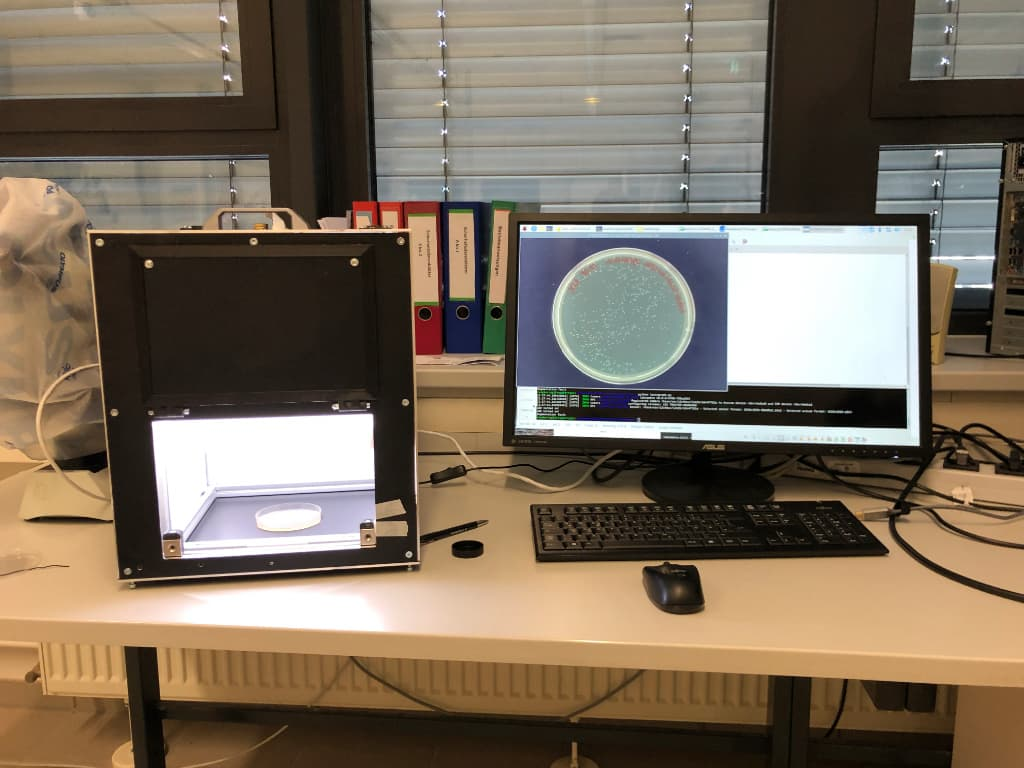
\includegraphics[height=6cm]{assets/photobox}
  \caption{Photo apparatus used to take images for the photobox dataset \cite{dehn2023identification}}
  \label{fig:photobox}
\end{figure}

The dataset contains plate images with different types of bacteria on different types of Agar. The colonies vary in shape, size, color and count. Some bacteria have a circular shape while others have mycelial growth (see top-right of Figure \ref{fig:image_types}). Some of the bacterial colonies have grown together, which makes it more difficult to segment them and count them accurately (in the center of top-middle in Figure \ref{fig:image_types}). Example images and the distribution of different types of images can be seen in Figure \ref{fig:image_types} and Figure \ref{fig:image_types_pie}.

\begin{figure}[hbt]
  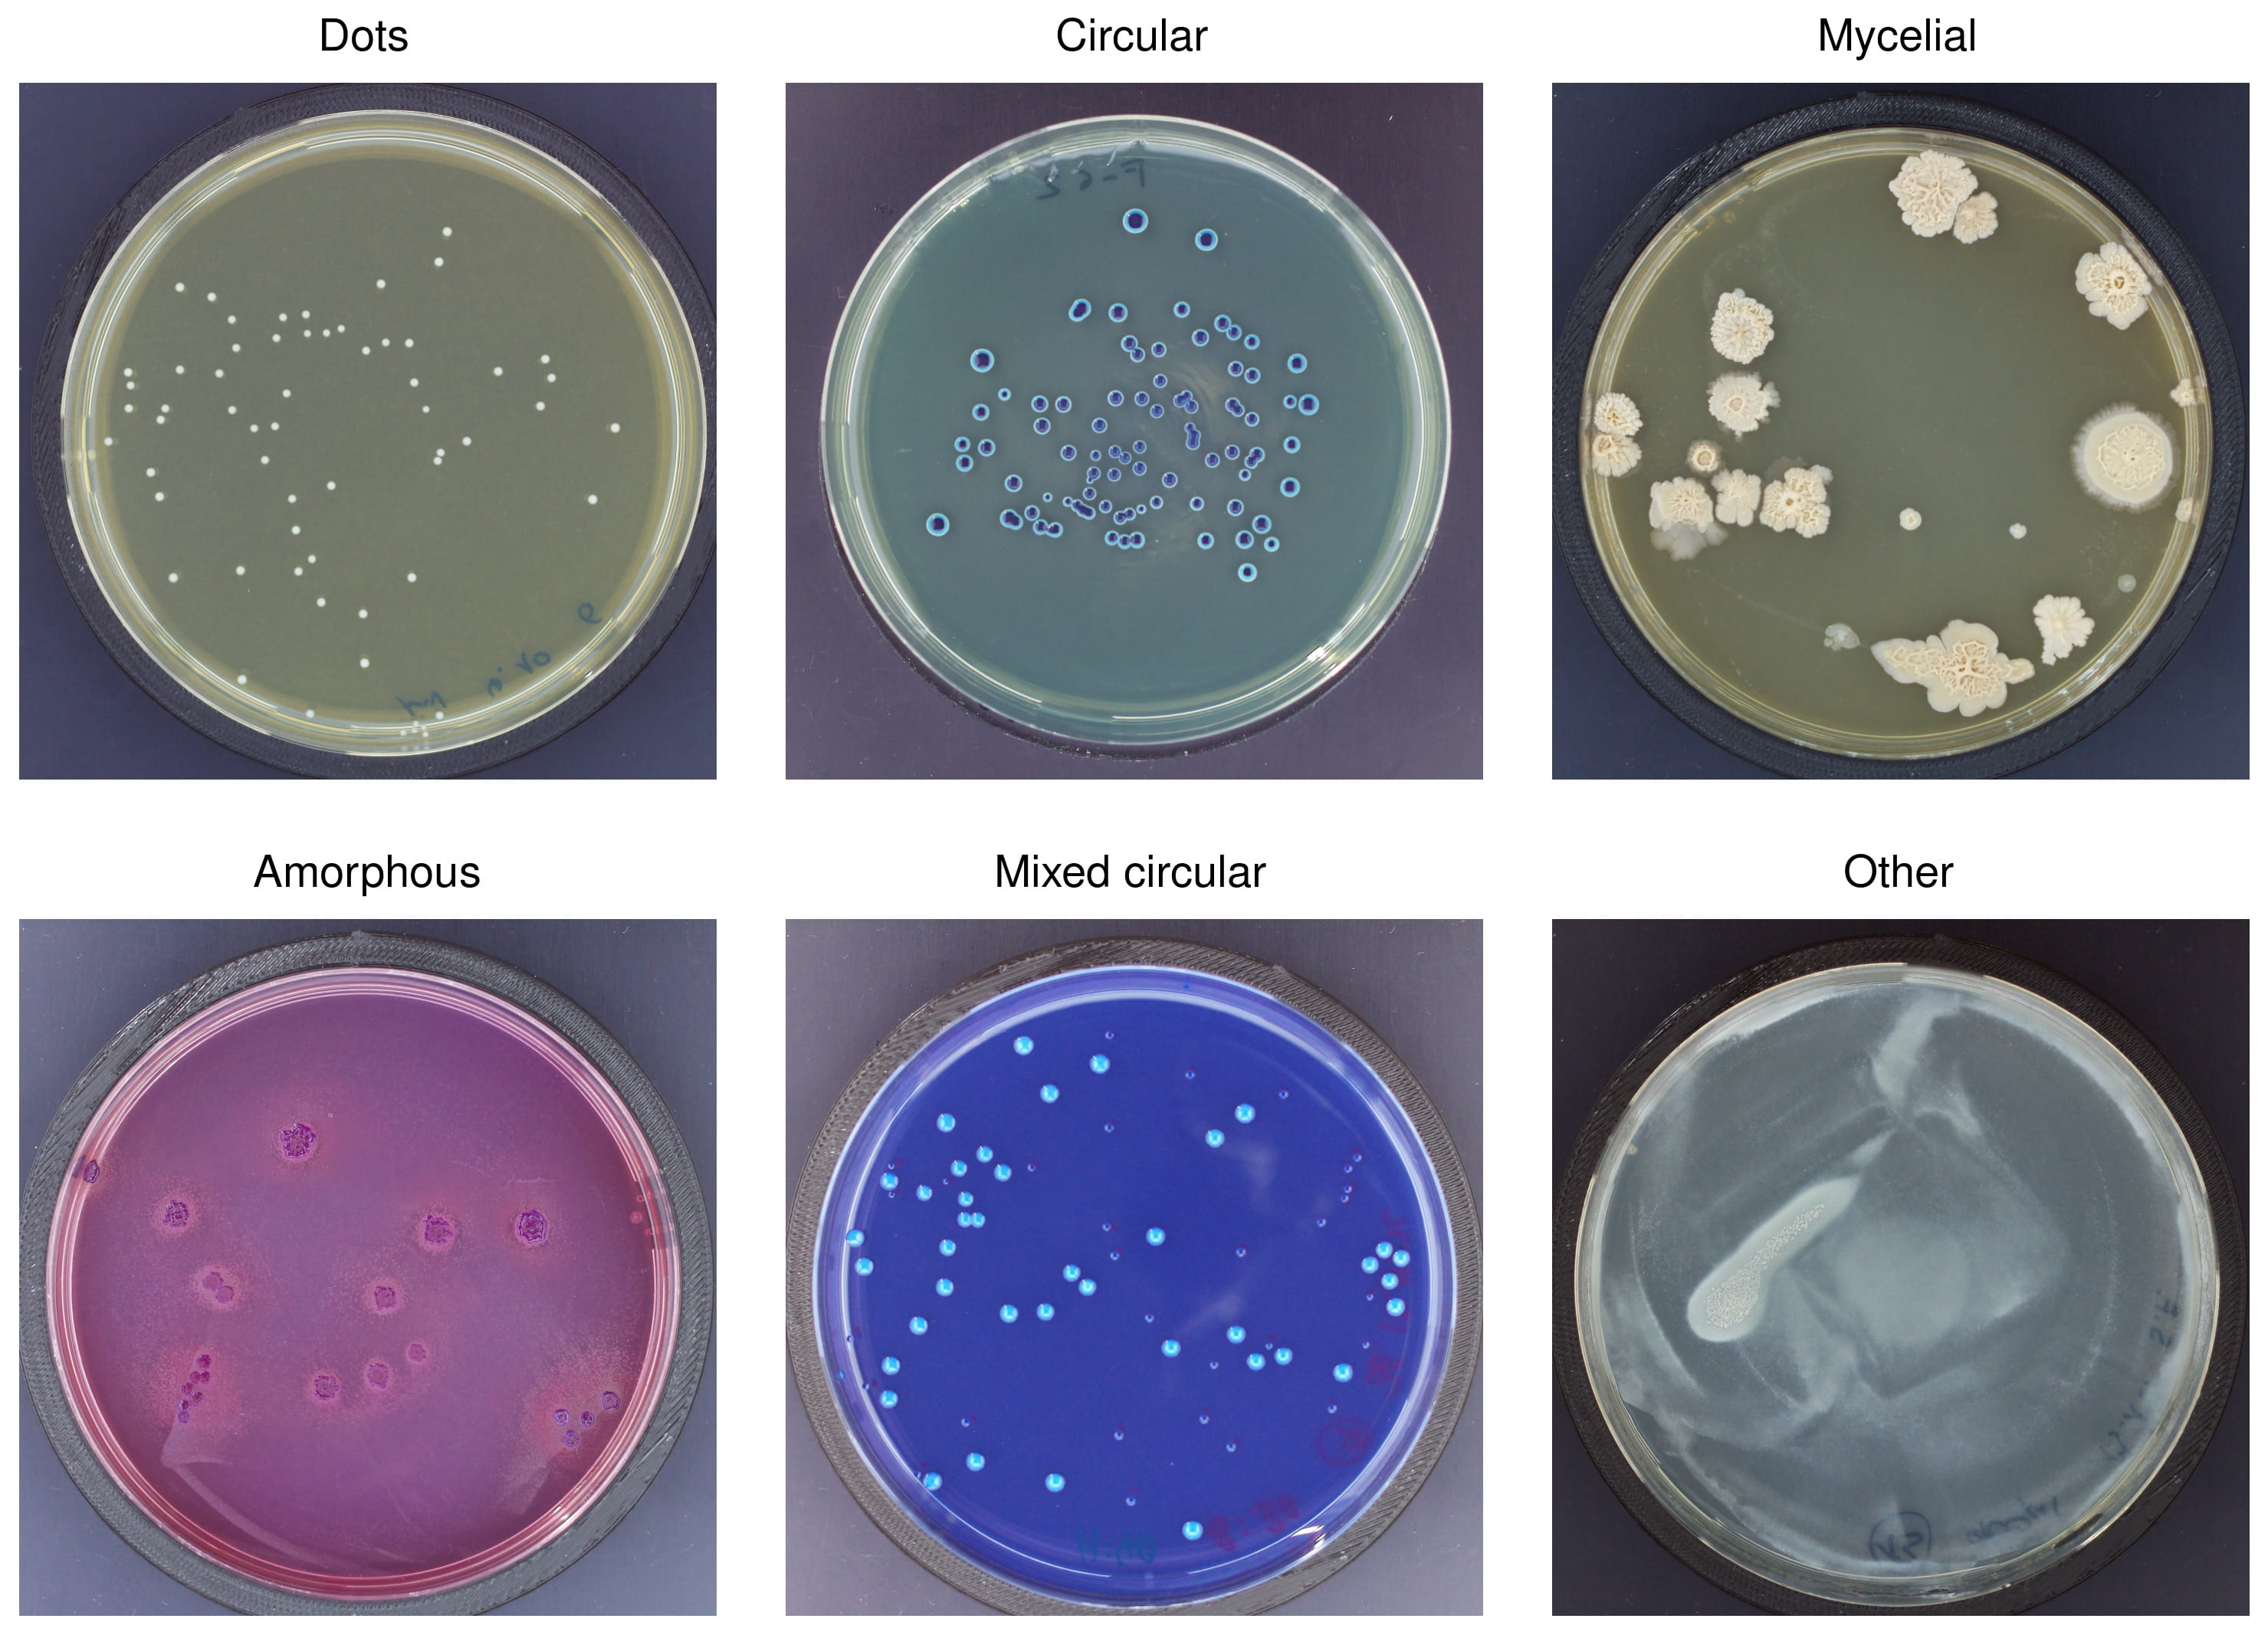
\includegraphics[width=\textwidth]{assets/chart_image_types}
  \caption{Overview of different types of images present in the photobox dataset}
  \label{fig:image_types}
\end{figure}

\begin{figure}[hbt]
  \centering
  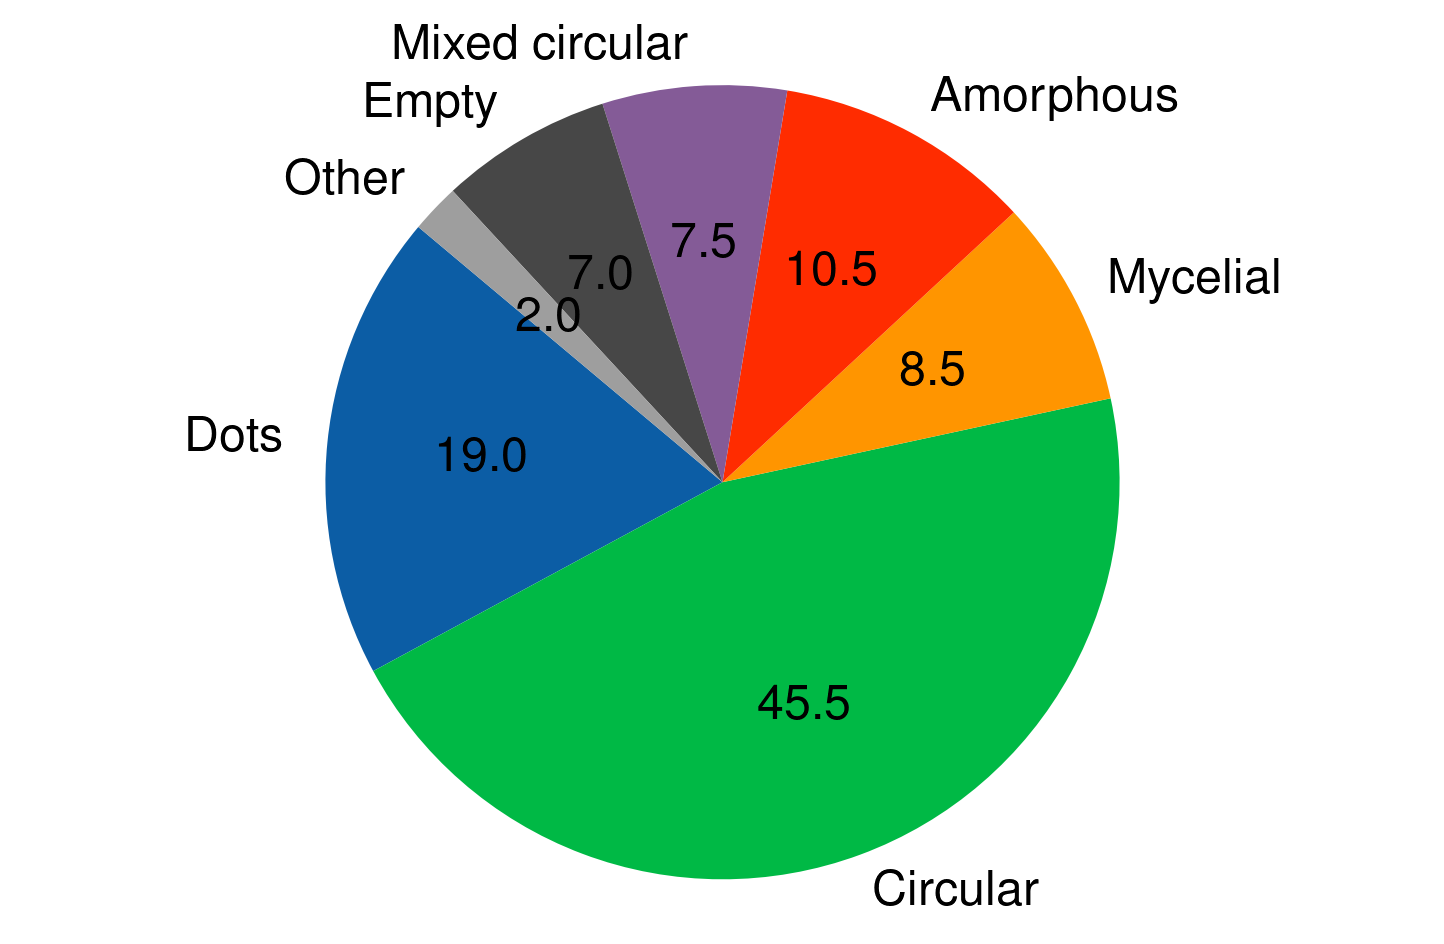
\includegraphics[height=6cm]{assets/chart_image_types_pie}
  \caption{Distribution of different types of images present in the photobox dataset}
  \label{fig:image_types_pie}
\end{figure}

Since the photobox dataset is of limited size, two other datasets were also used during model development. The first one is Microsoft COCO (Common Objects in Context), a large-scale dataset for object detection. It contains more than 200,000 annotated images in which 91 different object types are labeled with class labels, bounding boxes and segmentation masks. The categories include bench, suitcase, plate and sandwich and many more. \cite{lin2015microsoft} See Figure \ref{fig:coco_examples} for example images and masks.

Fine-tuning an object detection network pre-trained on the COCO dataset is a widely used technique to enhance model performance for small datasets, especially in medicine. \cite{sheng2020lymphoma} \cite{koitka2018ossification}

\begin{figure}[hbt]
  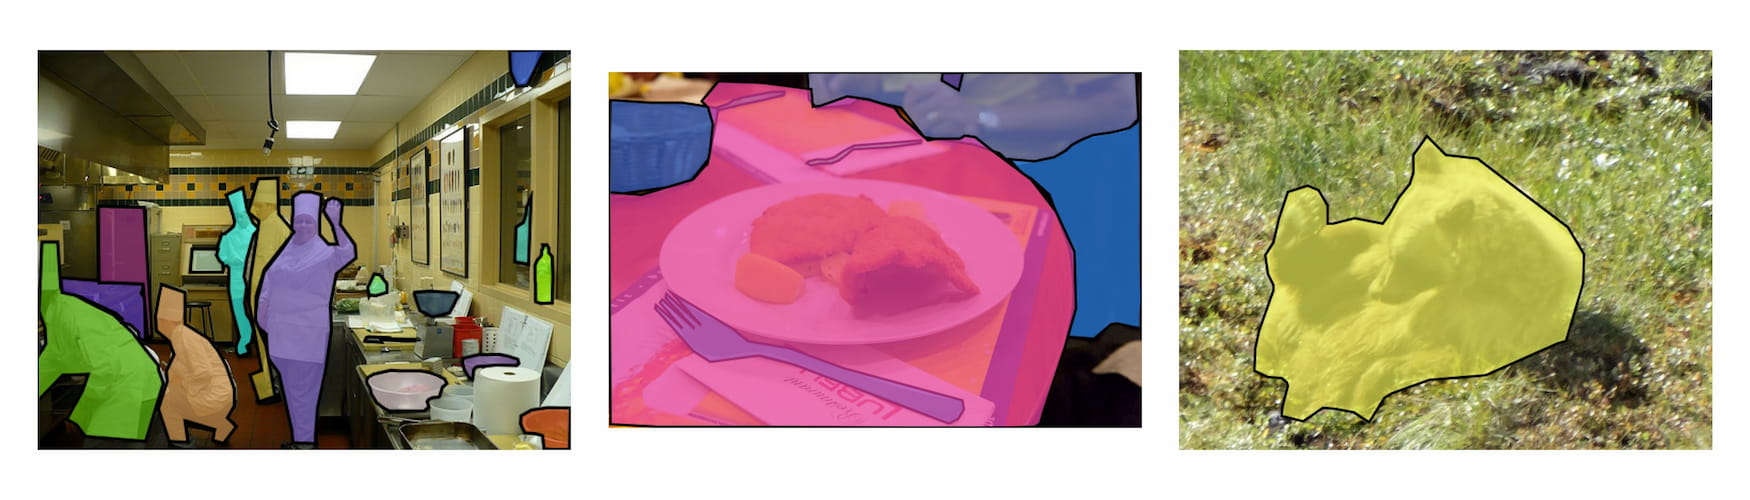
\includegraphics[width=\textwidth]{assets/chart_coco_examples}
  \caption{Example images with their corresponding masks overlayed \cite{cocodataset}}
  \label{fig:coco_examples}
\end{figure}

The second auxiliary dataset is the Annotated Germs for Automated Recognition dataset, AGAR for short. It contains 18,000 photos of five different microorganisms under different lighting conditions and in different resolutions. \cite{majchrowska2021agar} This dataset is highly related to the domain of this thesis.

Only the high-resolution subset of the AGAR dataset was used. There are 5242 train images and 1748 images for validation in this subset, each with a resolution of approximately 4000x4000 px (16 megapixels).

\section{Data Labeling}

\begin{figure}[h]
  \centering
  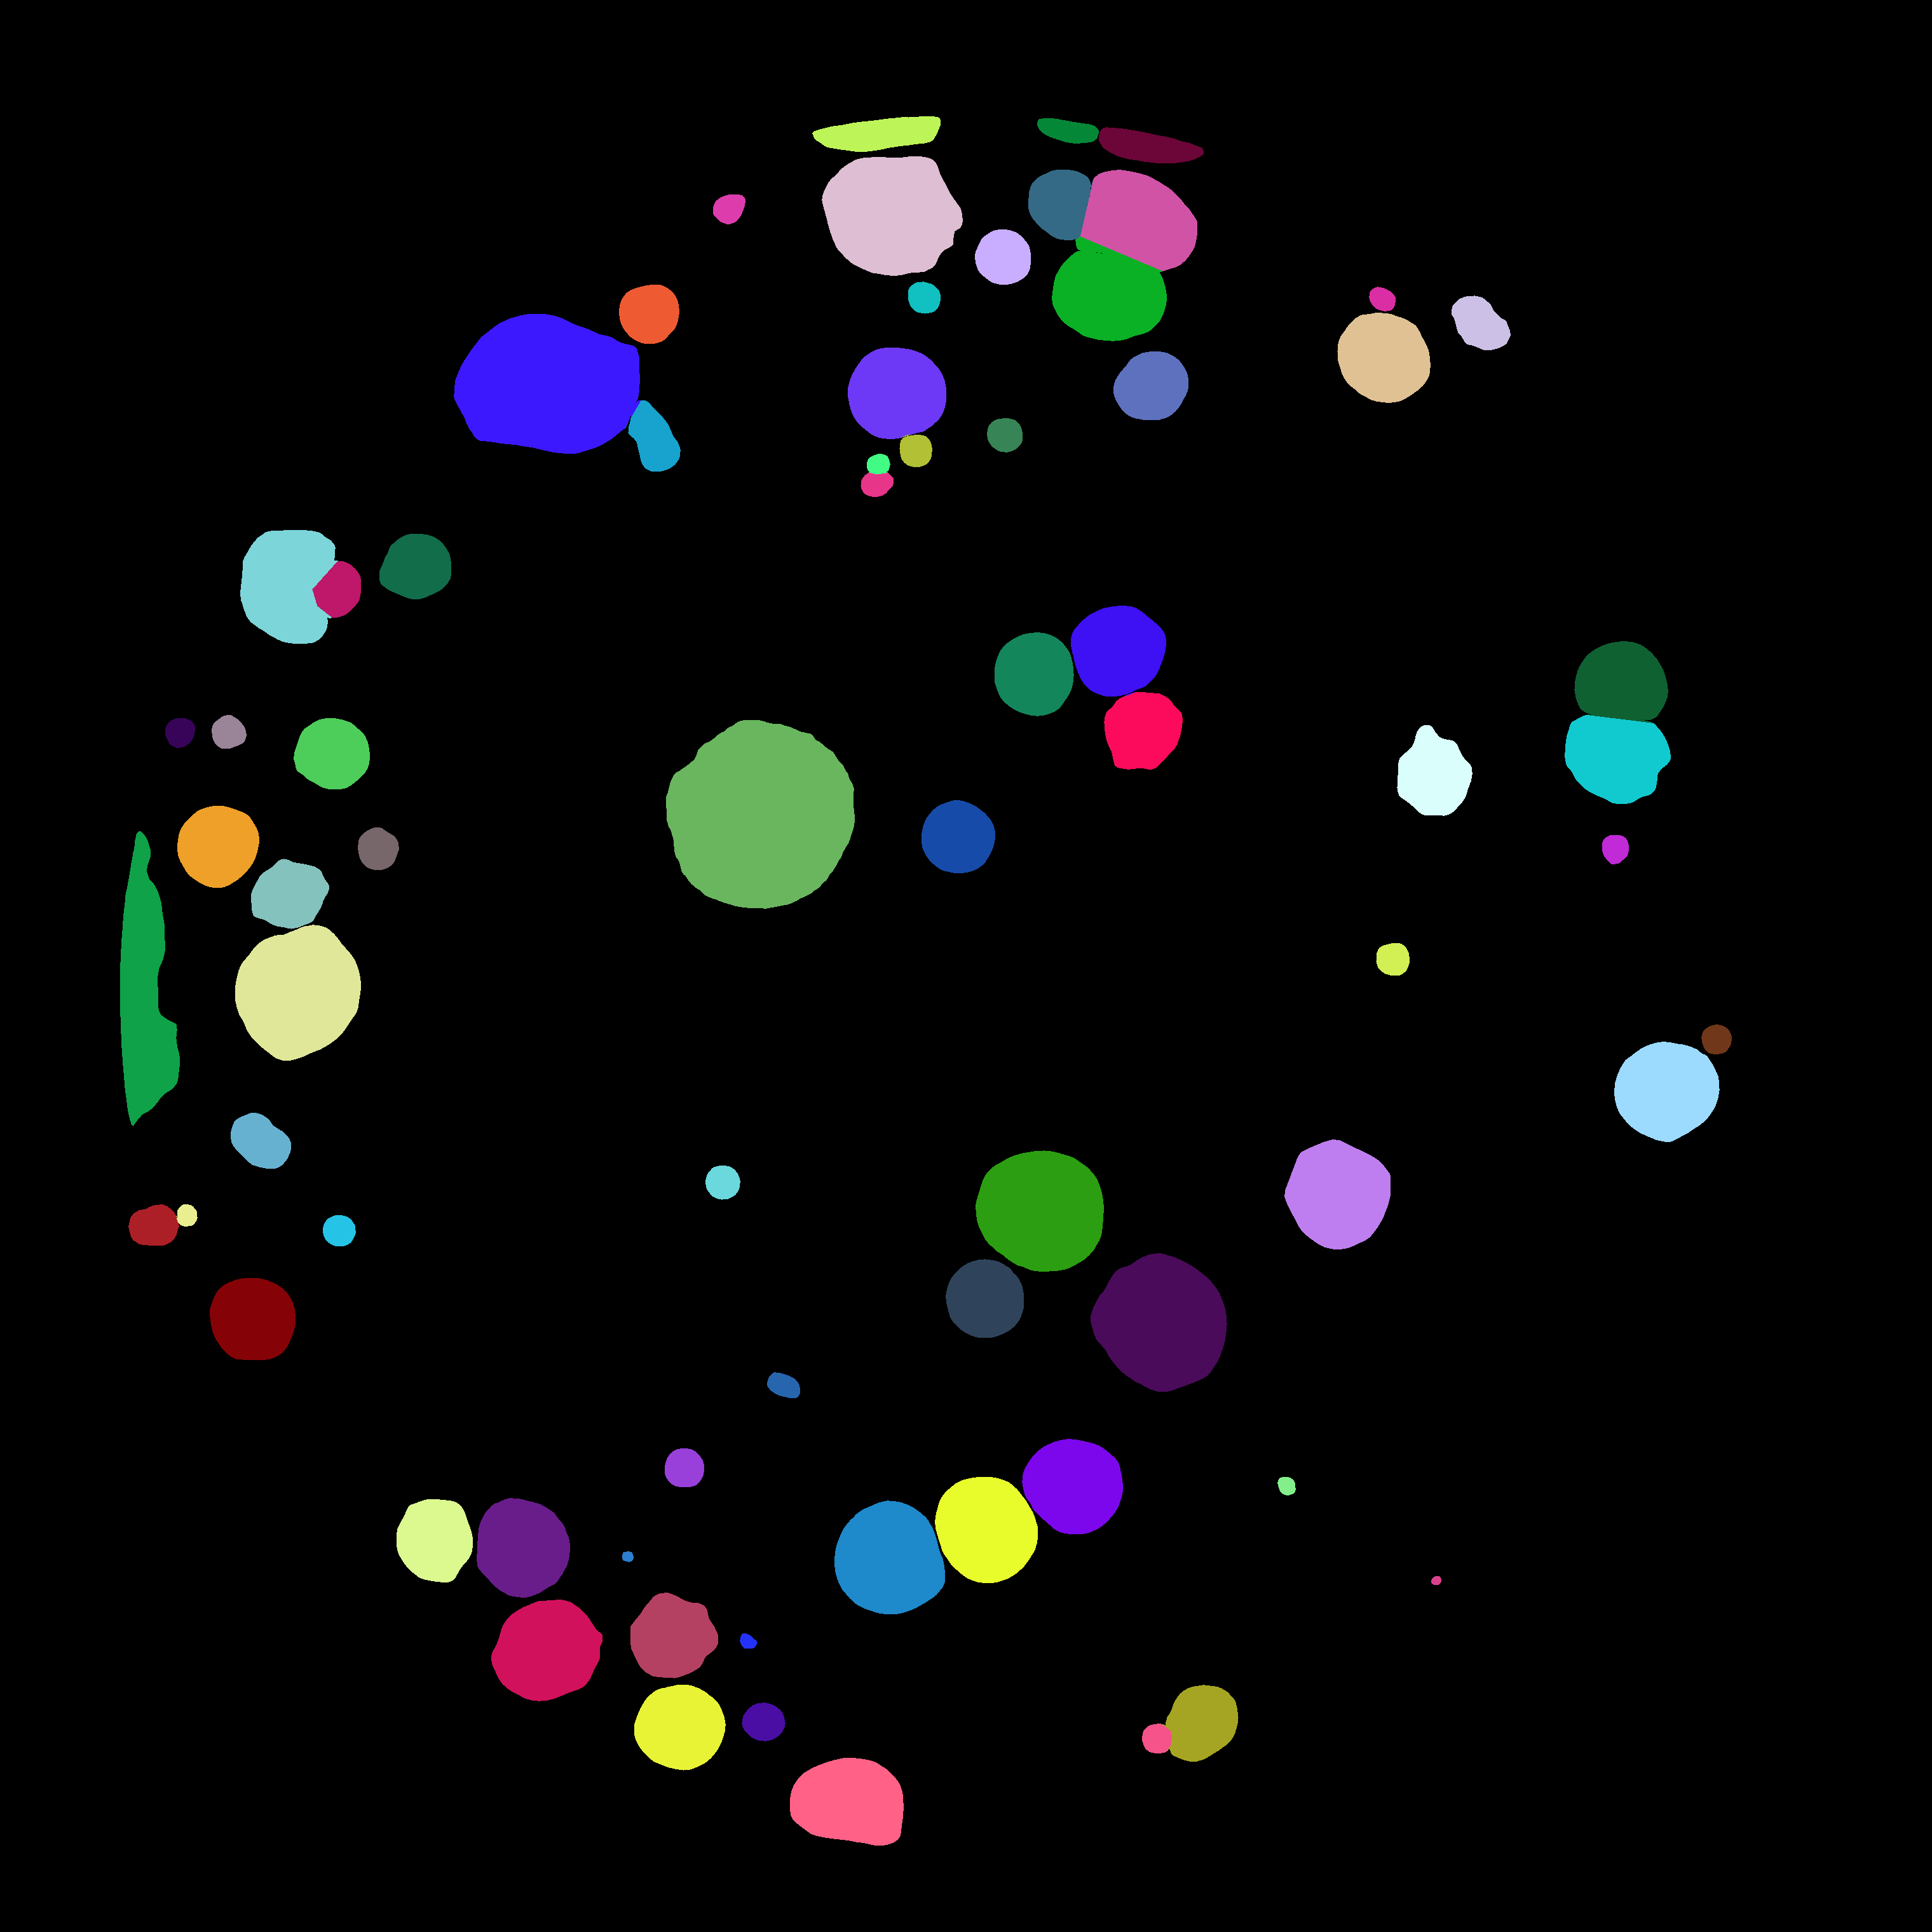
\includegraphics[width=0.4\textwidth]{assets/example_mask.png}
  \caption{Example of an instance segmentation mask}
  \label{fig:example_mask}
\end{figure}

Instance segmentation masks are selected as the type of label that is most useful for the photobox dataset. An instance segmentation mask here is a PNG image that has a black background with colored spots on it (see Figure \ref{fig:example_mask}). The colors are randomly chosen so no two colors are ever the same on a mask image and represent the individual instances (colonies).

Instance segmentation masks capture a lot of detail and can be trivially transformed into other types of datasets like bounding boxes, semantic segmentation masks or keypoints. This leaves room for experimentation, since the model architecture was not decided on yet.

To label the images of the photobox dataset, a web application was built as part of this thesis. The app (seen in Figure \ref{fig:annotation_app}) allows bulk upload of images on the left hand side. When an image is selected in the image browser on the left, it is analyzed on the server. Then accurate masks for each colony can be automatically created by clicking on the colony. By repeatedly clicking on every colony in the image, the full instance segmentation mask is created.

The automatic mask creation is built around the Segment Anything Model, SAM for short. SAM is a zero-shot image segmentation model for creating accurate segmentation masks from various prompts (see Figure \ref{fig:sam_task}). \cite{kirillov2023segment} It can mask objects from point locations, create a mask for an object contained in a bounding box or refine a rough mask to be more precise. The prompt for creating a mask when clicking on a colony in the labeling app is a point-prompt, which can be thought of as "please mask the object I am pointing at".

\begin{figure}[hbt]
  \centering
  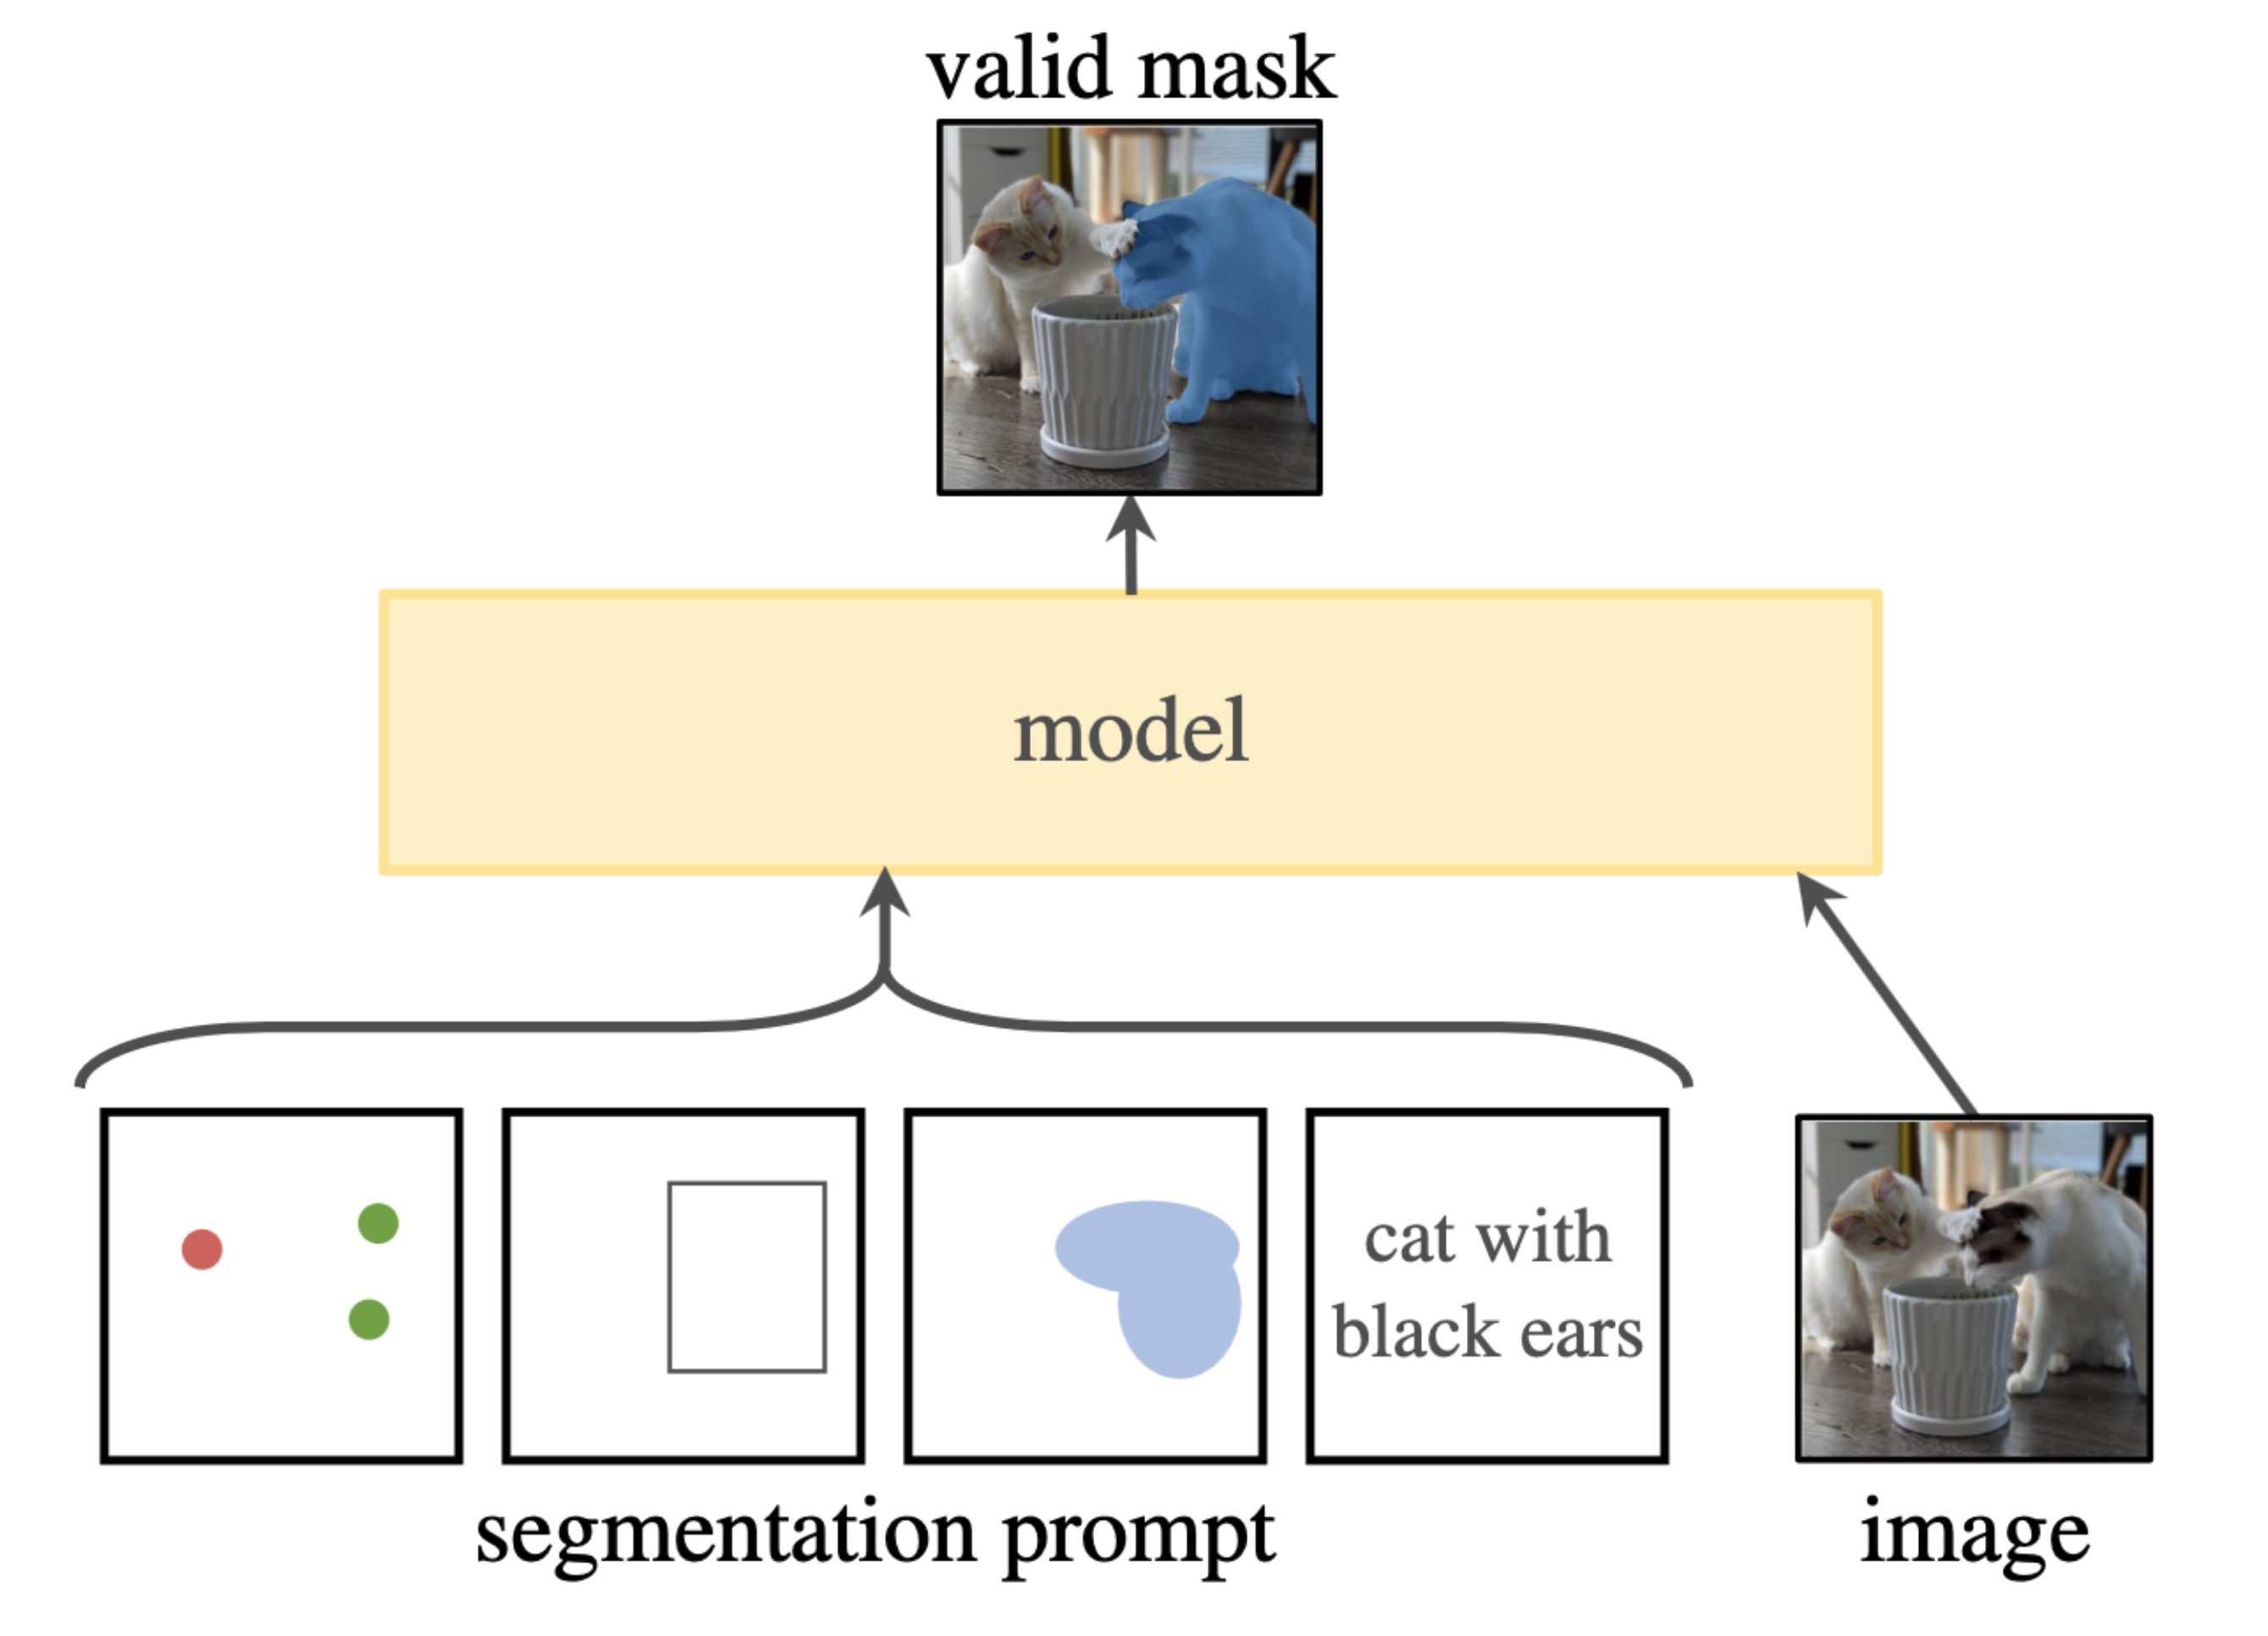
\includegraphics[width=0.5\textwidth]{assets/sam_task}
  \caption{Tasks SAM can perform \cite{kirillov2023segment}}
  \label{fig:sam_task}
\end{figure}

\begin{figure}[hbt]
  \centering
  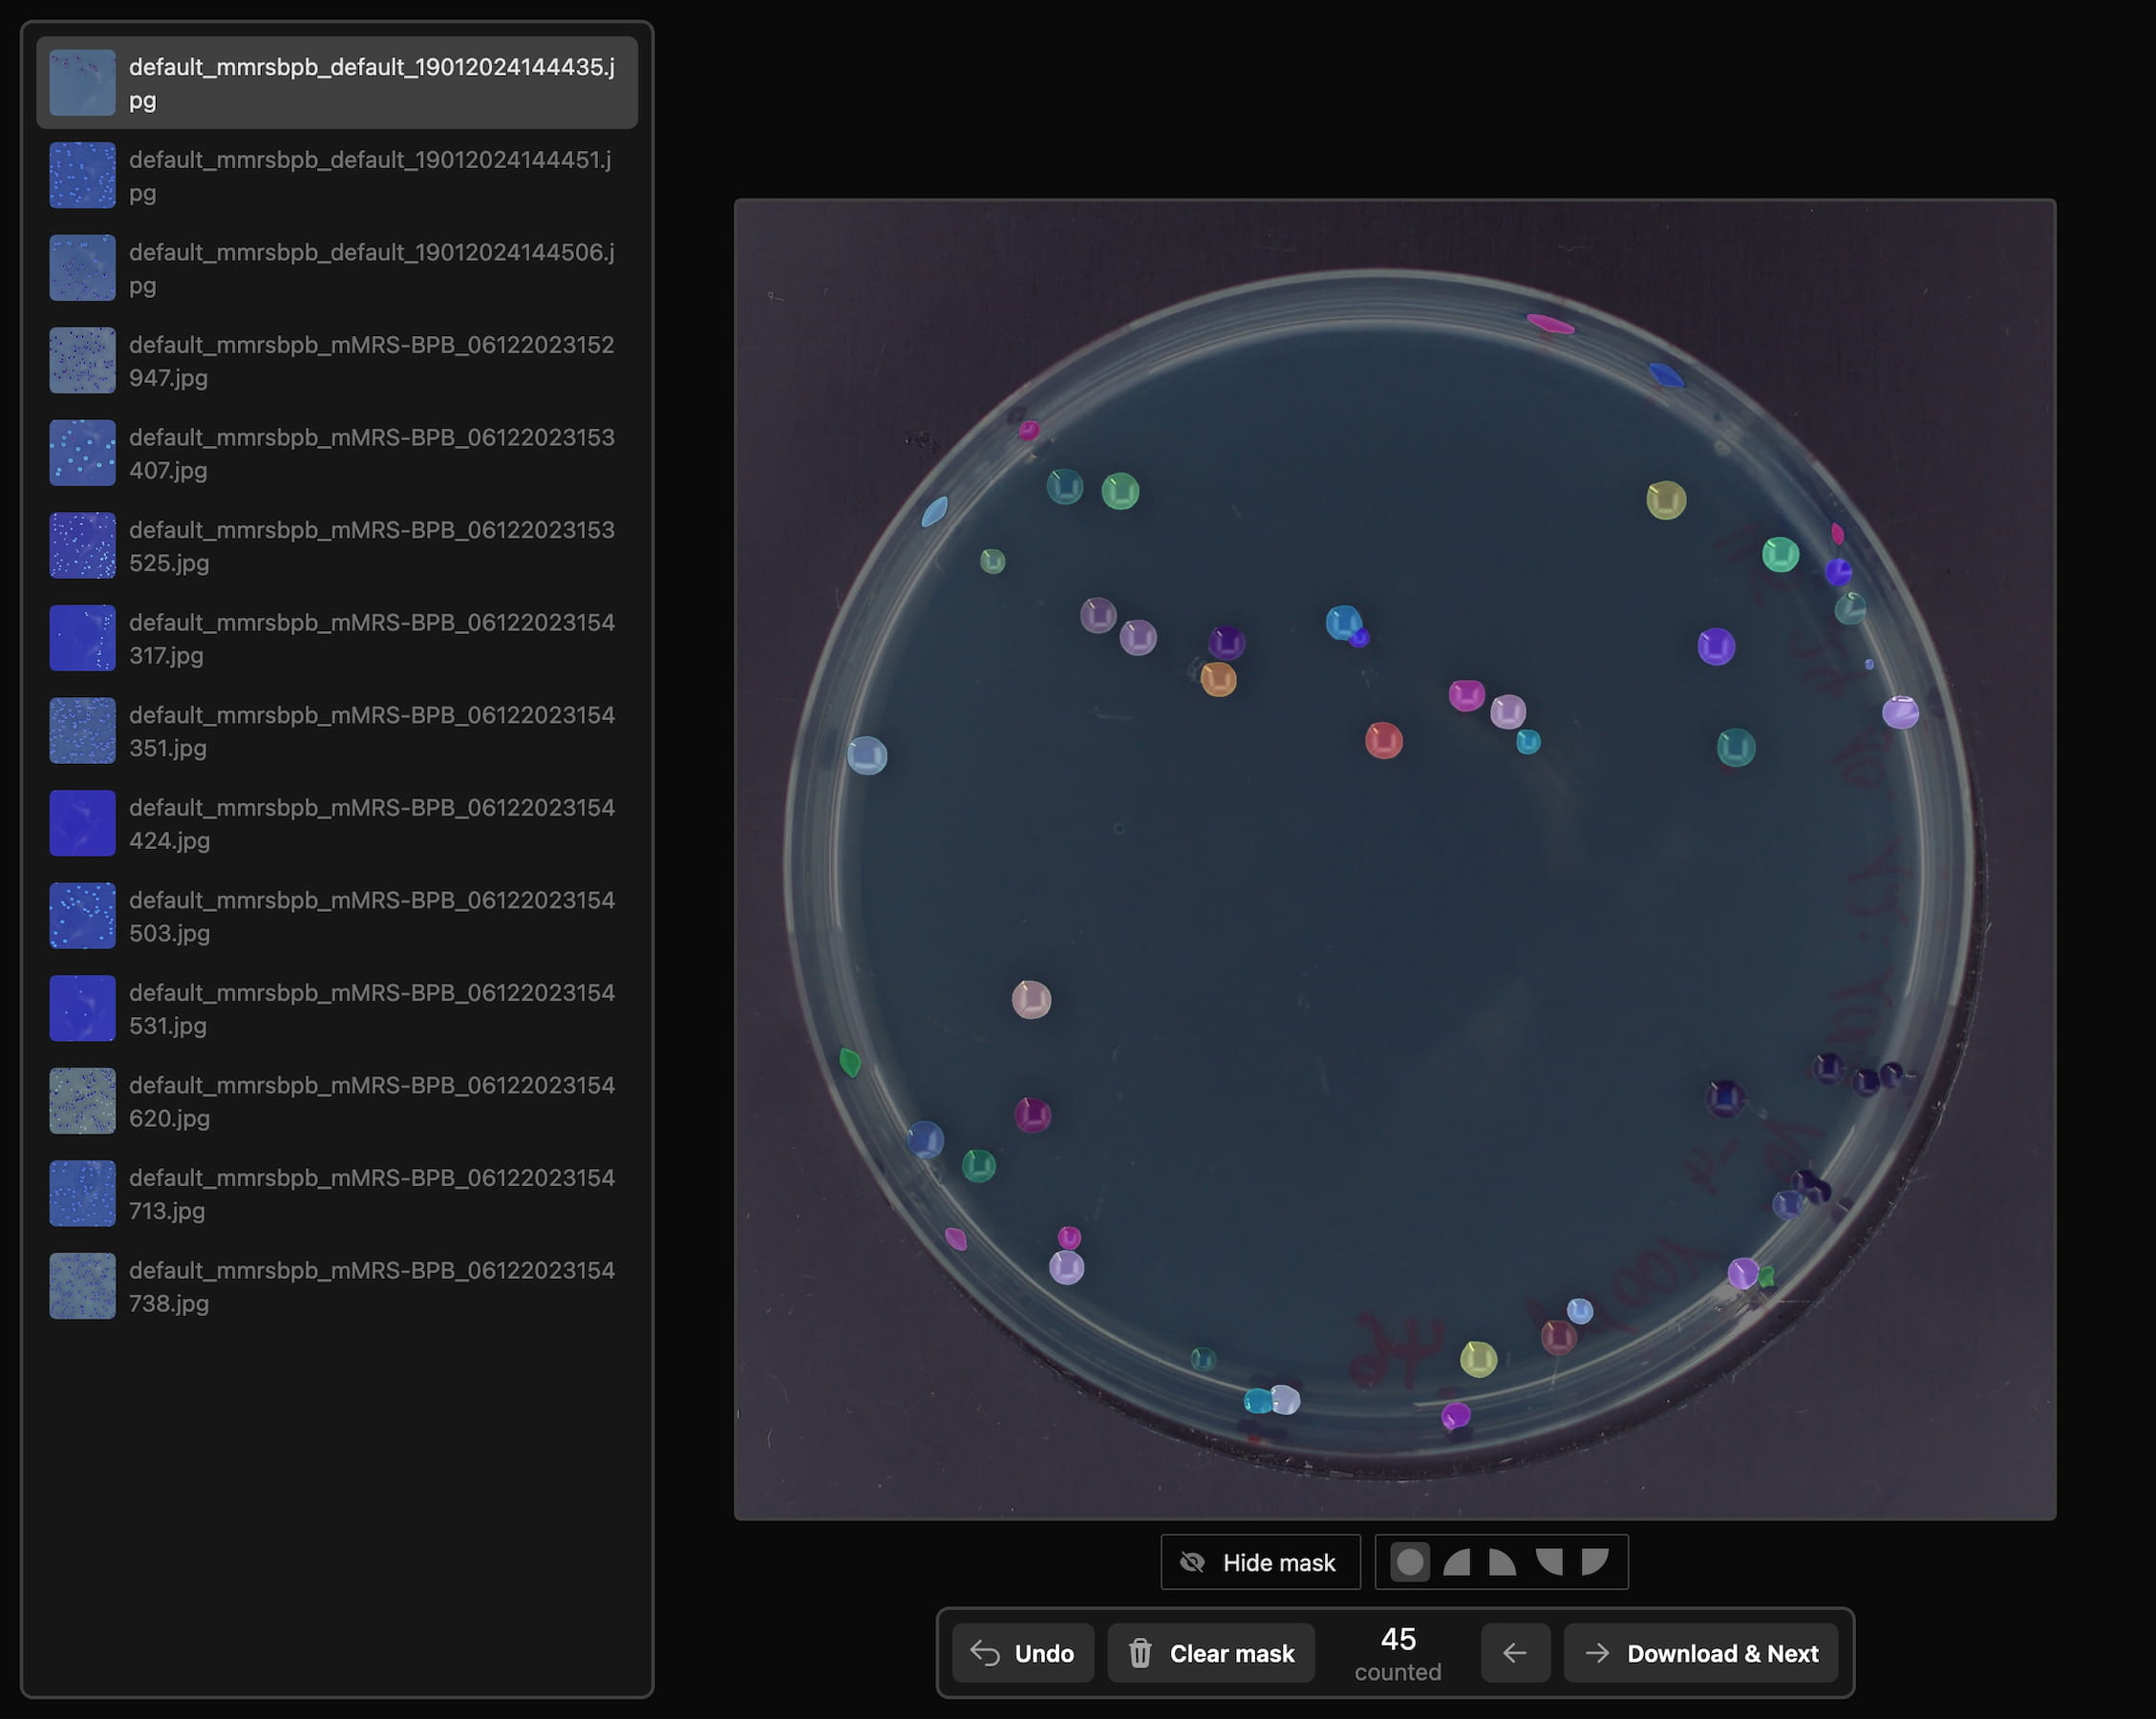
\includegraphics[width=0.8\textwidth]{assets/annotation-app-screenshot}
  \caption{Screenshot of the labeling app}
  \label{fig:annotation_app}
\end{figure}

This works well for most cases, however SAM can have difficulties fully masking a  colony if it has an irregular shape or is large in size (see top-right of Figure \ref{fig:image_types}). Normally, a new region is created for every click, which correlates to a new instance (i.e. not the same colony). But when multiple clicks are needed to capture a single colony because SAM fails to mask the full object, holding shift while clicking will add the newly masked area to the previous region (i.e. same colony).

Colonies that grew together are often collectively masked by SAM, but have to be accounted for independently. To separate this region it is possible to click inside of an existing mask to split it into two. Every pixel is then assigned to the mask of the click point it is closest to by using a k-d tree.

Other conveniences such as an undo button and zooming are also available. This setup of features allows every image in the photobox dataset to be labeled accurately. Manual correction of the masks, for example through photo editing software, is not needed.

The app is also deployed on a server at FH Münster, so their microbiology team can continue to grow their dataset independently.

\begin{figure}[hbt]
  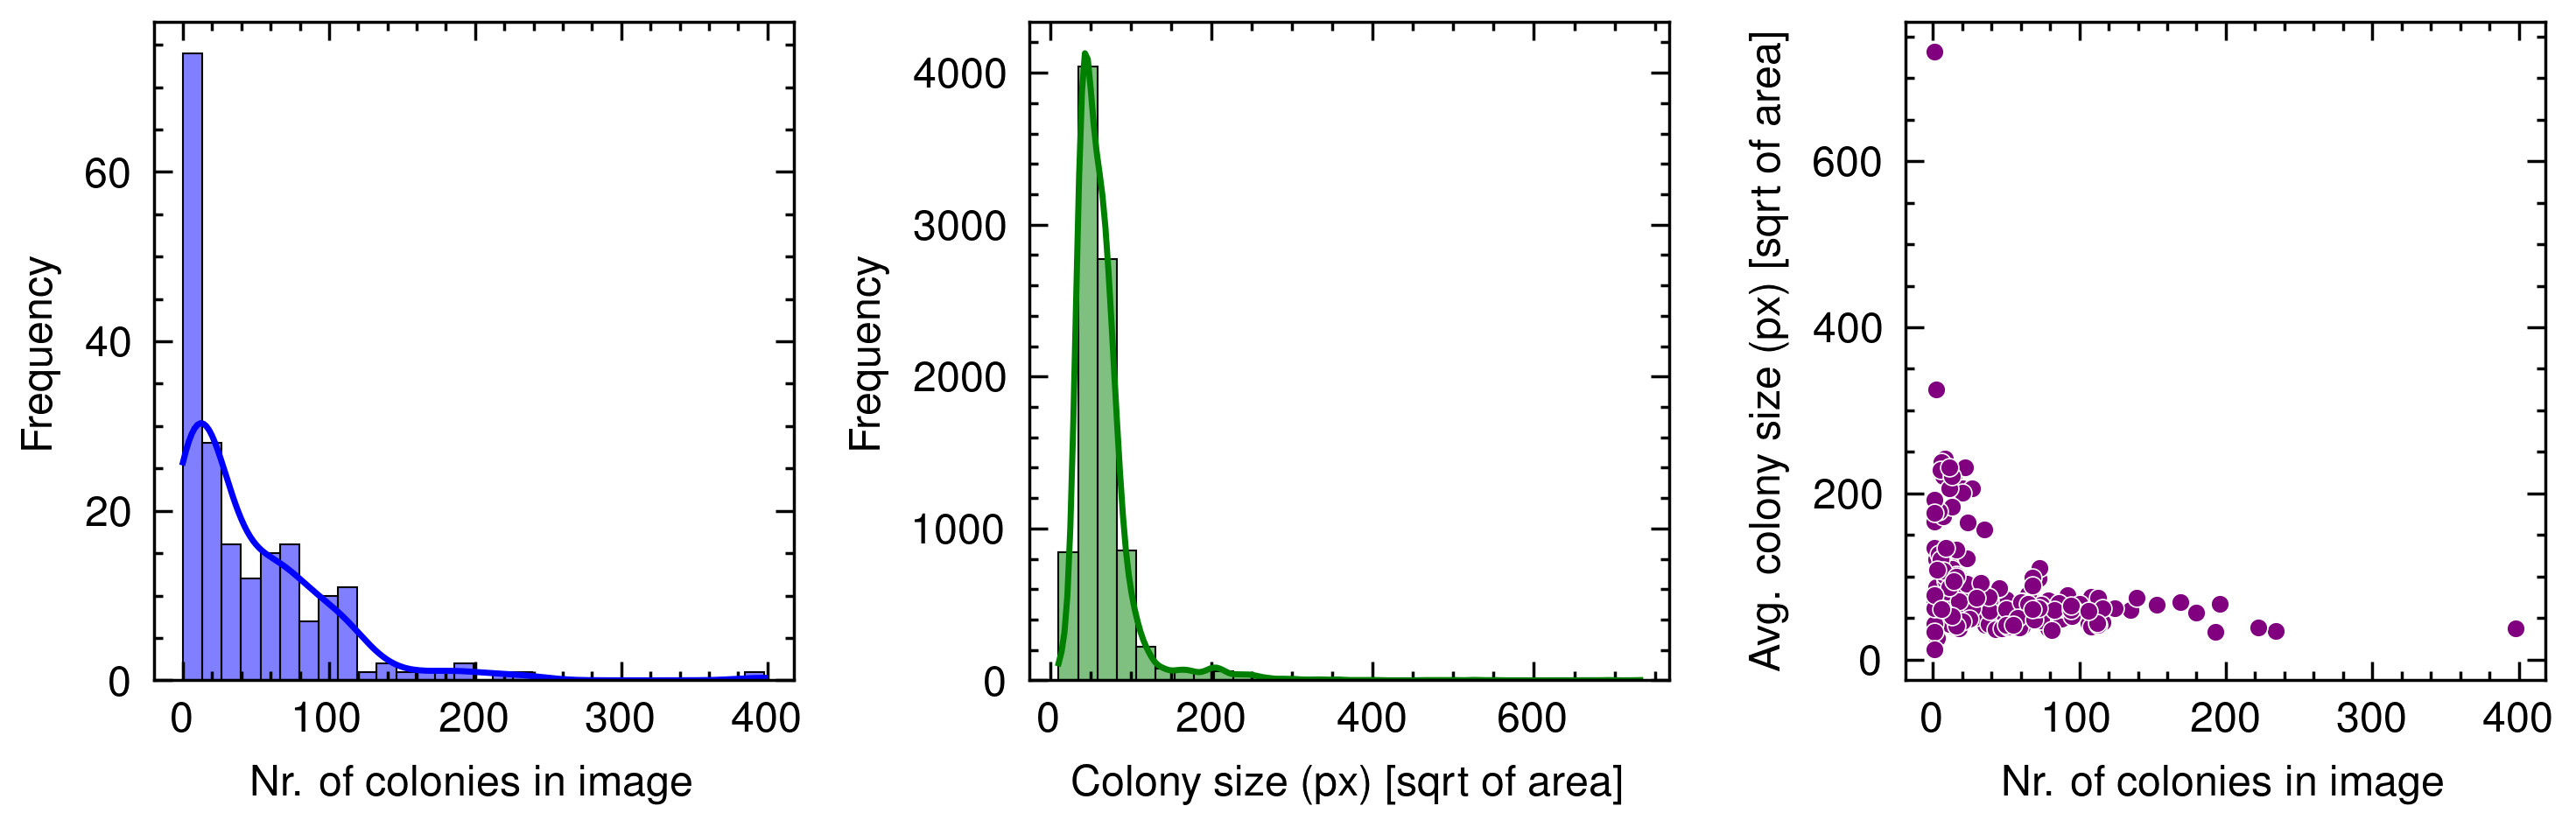
\includegraphics[width=\textwidth]{assets/chart_labeling_distribution}
  \caption{Distribution of the labeled data}
  \label{fig:labeling_distribution}
\end{figure}

Figure \ref{fig:labeling_distribution} shows statistics on the distribution of the created photobox dataset. The first histogram shows how many colonies are present on the images. It highlights a bias towards images with lower numbers of colonies, images with more than 200 colonies are rarely present. 

The second histogram shows the size of colonies in relation to their frequency in the dataset. It demonstrates that most of the colonies are of similar, smaller size, with a few outliers that are much larger, up to roughly 800x800 px. Such large colonies can be seen in the top-right image of Figure \ref{fig:image_types}.

The scatter plot on the right of Figure \ref{fig:labeling_distribution} shows the relation of the number of colonies in an image and the average size of the colonies in the image. It reveals a trend where images with fewer colonies can have colonies that are larger in size, but colonies on images with high counts are generally smaller.

\section{Data Preprocessing}

The photobox dataset is split into train, validation and test sets with a 50\%/25\%/25\% split. With the 200 labeled images that leaves 100 for training, 50 for validation and 50 for testing (performance evaluation).

The annotated instance segmentation masks are converted into a bounding box style dataset, similar to the AGAR dataset. Since each colony has a different color in the mask, it is easy to draw a bounding box around every region of unique color in the image. The pseudo code for this algorithm is outlined in \ref{alg:bb}.

\begin{algorithm}
\caption{Convert instance segmentation masks to bounding boxes}
\begin{algorithmic}[1]
\For{each mask in masks}
  \State unique\_colors $\gets$ get\_unique\_colors(mask)
  \For{each color in unique\_colors}
    \State $x1 \gets$ find\_first\_index(mask, color, 0)
    \State $y1 \gets$ find\_first\_index(mask, color, 1)
    \State $x2 \gets$ find\_last\_index(mask, color, 0)
    \State $y2 \gets$ find\_last\_index(mask, color, 1)
    \State save\_bounding\_box(mask\_id(mask), $x1$, $y1$, $x2$, $y2$)
  \EndFor
\EndFor
\end{algorithmic}
\label{alg:bb}
\end{algorithm}

For computer vision models it is common to use pre-processing image transformations, called augmentations, to artificially increase the dataset size. Here, several data augmentations are experimented with:

\begin{enumerate}
	\item Horizontal flip (50\% probability)
	\item Vertical flip (50\% probability)
	\item Random rotation of 0, 90, 180 or 270 degrees
	\item Shift brightness and contrast by up to 10\%
\end{enumerate}
 
A newly developed augmentation was also experimented with, inspired by the Random Cover Targets Algorithm proposed in \citet{biology11020156}. It is based around the idea of covering an area of the image that contains colonies and inpainting this area with the plate background. The new inpainted area now does not contain colonies and the corresponding mask can be filled with black in the inpaint area. This augmentation is referred to as the inpainting augmentation.

First, suitable areas for covering have to be found. The algorithm for finding these areas works by randomly positioning a circle on the image. It then checks if

\begin{enumerate}
	\item the circle is fully inside the area where colonies can occur (inside the plate, and not on the edge or in the corners of the image)
	\item the circle contains colonies (this is done by checking if there are non-black pixels in the corresponding mask)
	\item the circle does not "cut off" any colonies, i.e. a colony is half inside the circle and half outside
	\item the circle does not overlap more than 20\% with another circle that has been found
\end{enumerate}

The algorithm continuously tries to find such circles in an image. If no suitable circle was found within 1,000 tries, the circle finding program goes on to the next image. In total, 1,757 circles were found for the 100 images in the train set, on average 17.57 per image.

This brute force approach is fast enough, with somewhat optimized code it takes about 1 hour to find suitable circles for all images. It also finds enough circles for most images in its 1,000 tries and is statistically random, so each circle is as likely as any other to be generated (there is e.g. no bias towards circles that are closer to the center).

In the next step, for each image, each proposed circle would be covered individually. Then an image generation model was used to fill the covered area, a process known as inpainting. The goal of this step is to fill the area with background texture that matches the rest of the image.

The specific model used for inpainting is Kandinsky 2.2, specifically the inpaint variant published on Hugging Face. \cite{kandinskyhf} Kandinsky is a generative text-to-image model based around CLIP as the text and image encoder and latent diffusion. \cite{razzhigaev2023kandinsky} It can create realistic images from a text prompt, similar to DALL·E 2 \cite{ramesh2022hierarchical} and Stable Diffusion \cite{rombach2022highresolution}.

The text-to-image generation is guided by a positive prompt, which incentivizes certain elements to appear in the final image, and a negative prompt which specifies which elements should not be in the final image. When inpainting, the text-to-image model can only "control" the pixels included in the inpainting mask, so the context of the image is also important in guiding the generation.

The specific text prompts used for inpainting here are \textit{a clean petri dish with nutrient agar medium under laboratory lighting} for the positive and \textit{bacteria colony, bacterial colonies, bacteria, circles, dots, microbial spots} for the negative prompt. These prompts were constructed  through CLIP interrogation and experimentation. CLIP interrogation takes an image and gives a text prompt that when fed to a text-to-image model is likely to produce a similar image.

For the inpainting process the images are scaled down to 768x768 px, because that is the recommended image resolution for Kadinsky 2.2. They are upscaled to the original resolution of the images in the photobox dataset (3040x3040 px) using bicubic interpolation. The algorithmic upscaling has a blurring effect, but this can be neglected here since the area of interest from the generated image only contains background texture and no objects whose details would suffer from blurring.

The image generation often produces undesirable outcomes. A desirable inpainting result produces a texture that blends nicely into the background of the plate. However often the model will generate additional colonies into the image or even produce artifacts (see Figure \ref{fig:messed_up_generation}). Therefore each generated image has to be checked, which takes about 2.5 hours to sort manually for the 1,757 generated images. 

\begin{figure}[h]
  \centering
  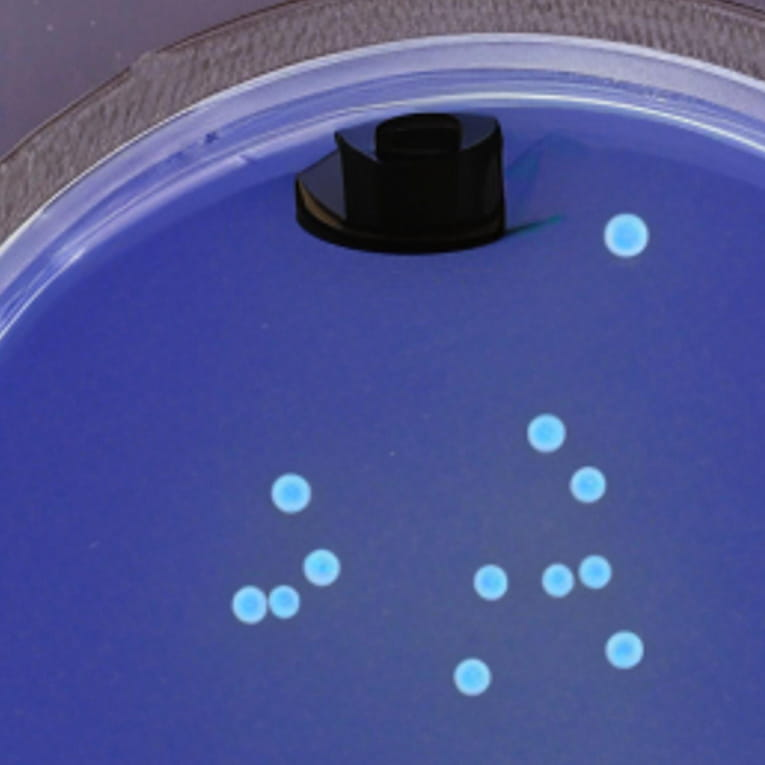
\includegraphics[width=0.24\textwidth]{assets/messed_up_generation.jpg}
  \caption{Example of an artifact generated during the inpainting process}
  \label{fig:messed_up_generation}
\end{figure}

Sorting out the images with undesirable outcomes leaves 934 images which can be used for augmenting the dataset. These can now be used to cover up the colonies in an original image, by copying in the inpainted area from a generated image. An example of this process can be seen in Figure \ref{fig:inpaint}. 

\begin{figure}
     \centering
     \begin{subfigure}[b]{0.4\textwidth}
         \centering
         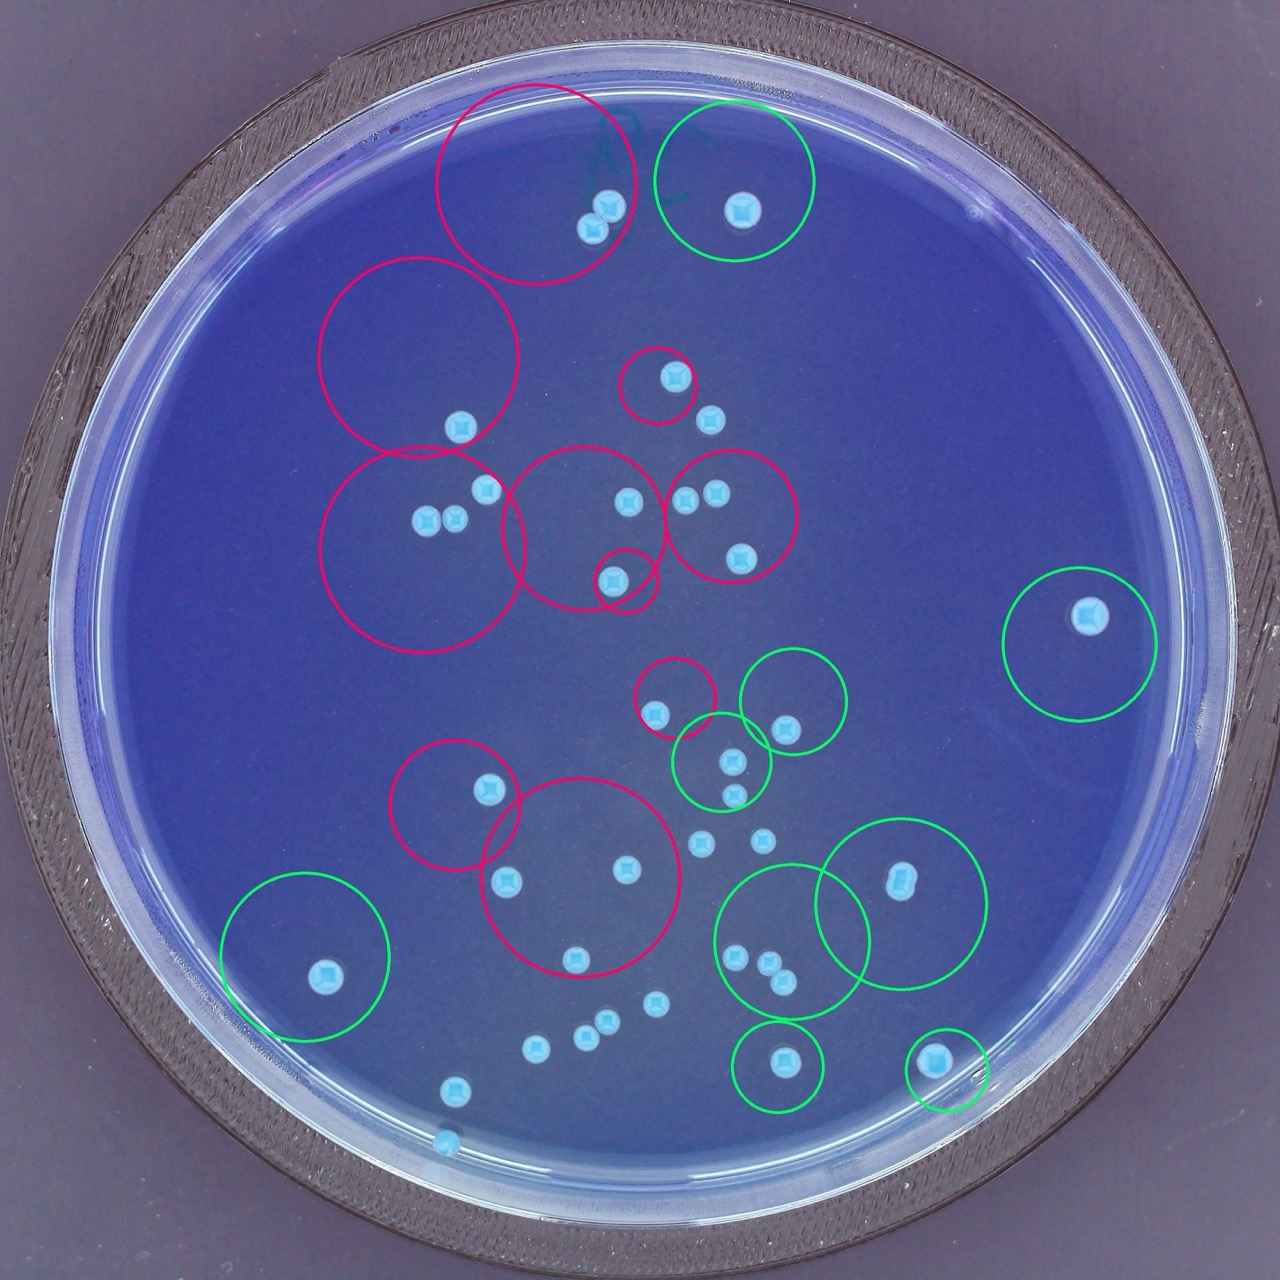
\includegraphics[width=\textwidth]{assets/circles_visualized}
         \caption{Potential inpainting circles. Green ones can be kept, red ones are undesirable.} 
         \label{fig:circles_visualized}
     \end{subfigure}
     \begin{subfigure}[b]{0.4\textwidth}
         \centering
         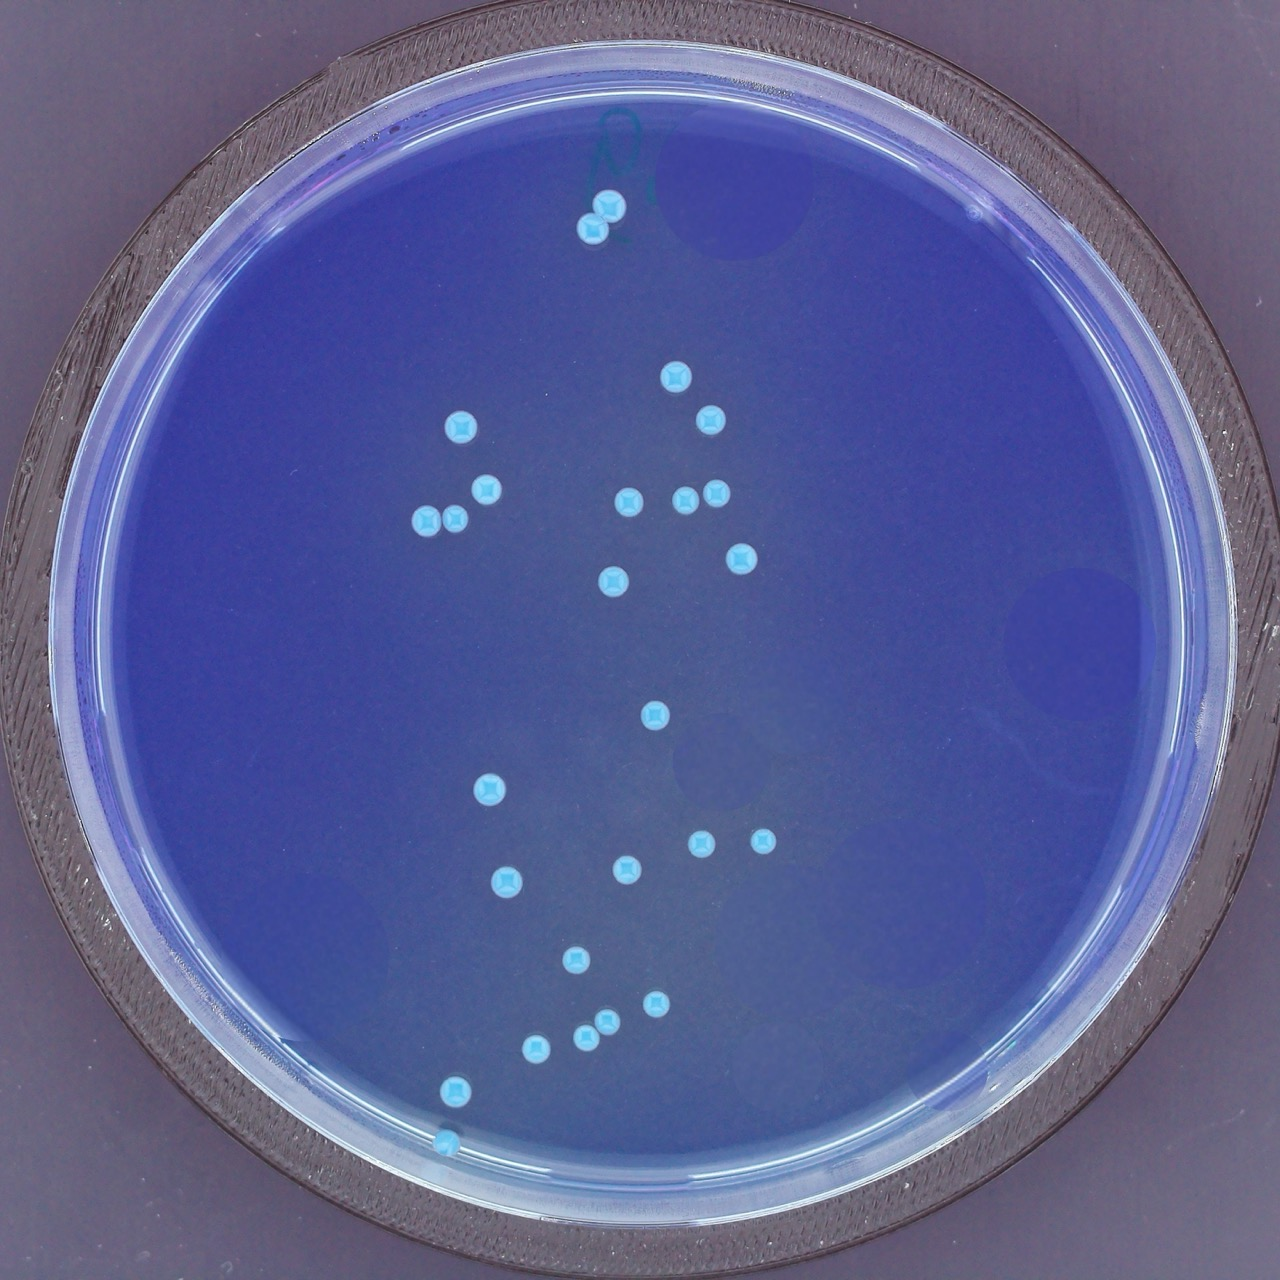
\includegraphics[width=\textwidth]{assets/inpaint_circles_applied}
         \caption{All successful inpainted circles are copied onto an original image.}
         \label{fig:inpaint_circles_applied}
     \end{subfigure}
     
        \caption{Patch augmentation pipeline for an example image}
        \label{fig:inpaint}
\end{figure}

During training, when an image is loaded for a forward pass through the model, each patch is loaded with a chance of 50\%. When a patch is loaded, the bounding boxes contained in the circle area are removed from the labels. Loading a patch can be thought off as toggling a layer in photo editing software.

\section{Model Development}

As explained in the introduction, the goal of this work is to localize all colonies on the plate individually and being able to count them. 

An object detection model is best suited for this job because it is able to localize bounds of each colony, which a regression based (directly predicting the number of colonies from an image) or density map based counting model could not. It is also able to distinguish individual colonies, even if they overlap, which a semantic segmentation model (is this pixel a colony or not?) could not. Instance segmentation models, which create output masks just like the labels of the photobox dataset (see Figure \ref{fig:example_mask}) would also work. But object detection models are easier to train and the mask output is not needed.

From the family of object detection models, Faster R-CNN was selected as the architecture for this project. Faster R-CNN is a two-stage object detection model. A region proposal network and a classifier work on feature maps created by a backbone model (here ResNet-50). The region proposal network creates proposals for regions that could contain an object of interest, the classifier then decides if the object belongs to the background or any of the specified classes. \cite{ren2016faster} Figure \ref{fig:faster_rcnn_architecture} shows the architecture in a diagram. In this work, there are only two classes, one for background (not of interest) and one for colony. This could however be easily expanded to classify colonies by species during the detection process.

Faster R-CNN has a readily available PyTorch implementation \cite{PyTorchVision_FasterRCNN} which includes pre-trained weights for the COCO dataset based on the training approach from \citet{li2021benchmarking}. As shown in \citet{Majchrowska_2022}, the difference in performance between state-of-the-art object detection models on the task of microbial colony detection is minimal. So Faster R-CNN is a good choice since the effort of implementing a training script \cite{torchvisiontutorial} and using pre-trained weights \cite{fasterrcnnweights} is much reduced.

\begin{figure}[hbt]
  \centering
  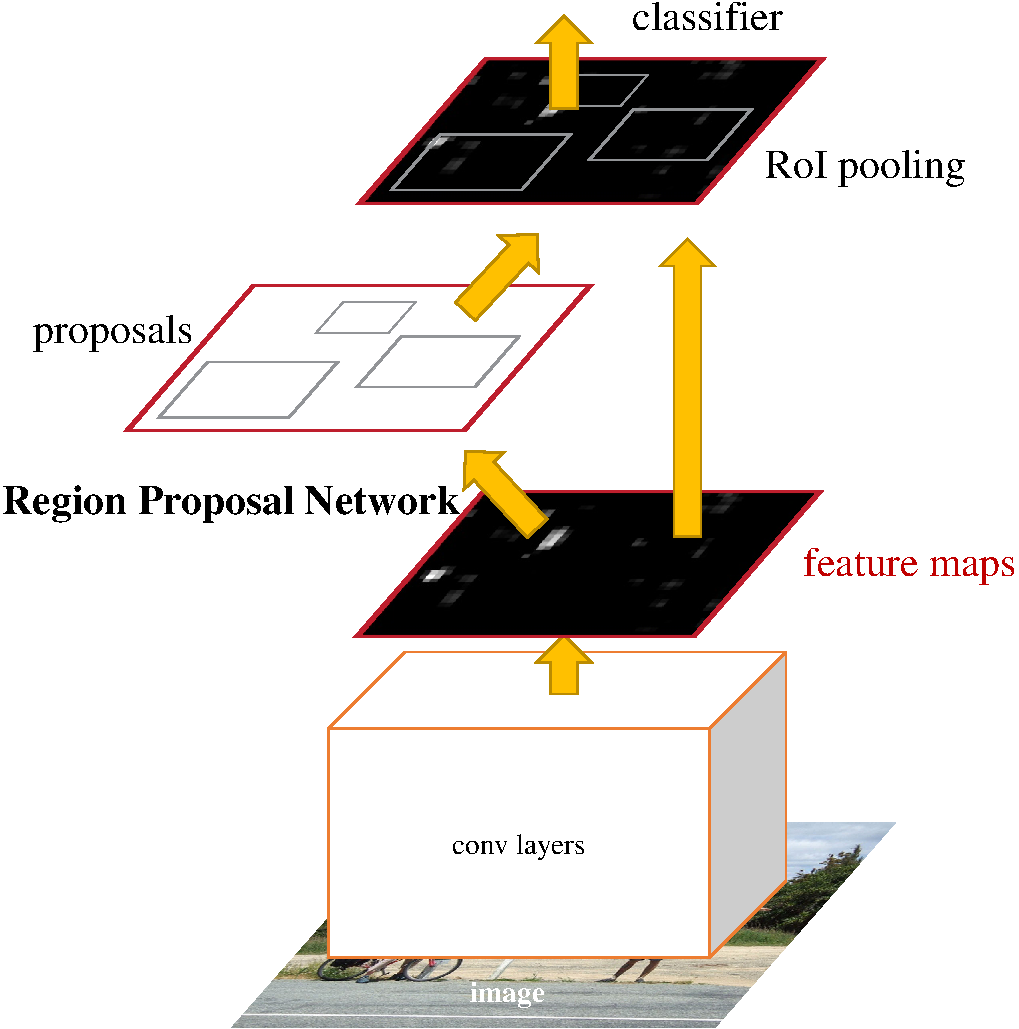
\includegraphics[width=0.5\textwidth]{assets/faster_rcnn}
  \caption{Overview of the Faster R-CNN architecture \cite{ren2016faster}}
  \label{fig:faster_rcnn_architecture}
\end{figure}

The model is optimized by stochastic gradient descent, using a momentum of $0.9$ and a weight decay of $0.0005$. The learning rate is initialized to $0.005$ for a batch size of 8. The learning rate was scheduled with a ReduceLROnPlateau strategy, which would cut the learning rate by 90\% after no improvements have been made to validation loss for 10 epochs. After the learning rate has been reduced two times, training stops. This eliminates $n_{epochs}$ as a hyperparameter that needs tuning and makes experiments easier.

All training runs are conducted on single nodes from the Campus Cluster of FH Münster equipped with Tesla V100 16GB graphics cards.

\subsection*{Evaluation Metrics}

Before discussing the different experiments, the metrics used for evaluating an experiment have to be laid out. Accurately counting the colonies is the primary focus of this work and precisely locating them is of secondary interest, the main metrics used for evaluating are comparing the number of detected colonies vs the ground truth. They are adapted from \citet{majchrowska2021agar}.

The symmetric mean absolute percentage error metric, sMAPE for short, measures relative counting error in relation to the amount of colonies on the plate.

\[
\text{sMAPE} = \frac{1}{N} \sum_{i=1}^{N} \frac{|x_i - \tilde{x}_i|}{|x_i + \tilde{x}_i|}
\]

Here $N$ is the number of images, $x_i$ is the number of colonies on the image and $\tilde{x}_i$ is the colonies in a prediction. For the case of $x_i=\tilde{x}_i=0$, meaning there are no colonies on the image and the predicted colony count is 0, nothing is added to the sum as the prediction is correct.

The mean absolute error, MAE for short, is the mean over all absolute counting errors for predictions on images of the test set, so

\[
\text{MAE} = \frac{1}{N} \sum_{i=1}^{n} | x_i - \tilde{x}_i |
\]

As an object detection metric, mean average precision, mAP for short, was used. The average precision is the area under the precision-recall-curve. To draw a precision-recall-curve, these values have to be calculated:

\begin{description}
  \item[True positives] (TP) are predictions the model has made, which are correct (match a ground truth bounding box).
  \item[False positives] (FP) are predictions the model has made, which are incorrect (do not match a ground truth bounding box, are duplicates, etc.).
  \item[Precision] is $\frac{TP}{TP + FP}$, i.e. how much of the predictions are actually correct.
  \item[False negatives] (FN) are cases where a prediction should have been made, but is missing.
  \item[Recall] is $\frac{TP}{TP + FN}$, i.e. how much of what should have been found has been found.
\end{description}

The precision recall curve is drawn by going through each predicted bounding box sorted by confidence score, and calculating precision and recall for the subset of bounding boxes that have been "visited". When plotting these values onto a graph with precision on Y and recall on X axis and connecting all of them, the area under the curve is the average precision.

Deciding between a true and a false positives for an object detection model requires setting an IoU threshold. The Intersection over Union, short IoU, is the area of the overlap between two boxes divided by the area of the union of both boxes. The IoU threshold is a fixed number that determines whether a detected box is correct.

Mean average precision is the mean of the average precision at different IoU thresholds, here it is every IoU threshold between 0.5 and 0.95 with steps of 0.05. This is also the primary metric for comparing performance of object detection models on the COCO dataset. \cite{cocoevaluation} It's score is indicative of how well a model can detect the objects it is supposed to detect, and how precisely it can locate them.

\subsection*{Experiments}

For the experiments, evaluation metrics are calculated for the validation set. Comparisons are always against a model trained from random initial weights.

First, the rotation augmentation was tested for its impact on performance. As mentioned before, the random rotation augmentation randomly rotates an image during training by 0, 90, 180 or 270 degrees.

\begin{table}[h]
\centering
\begin{tabular}{lcccc}
\hline
  & mAP & MAE & sMAPE \\
\hline
Rotation enabled  & 0.6869 & 11.36 & 0.2743 \\
No Rotation  & \textbf{0.6919} & \textbf{9.7} & \textbf{0.2492} \\
\hline
\end{tabular}
\caption{Comparison of metrics with and without rotation}
\label{table:rotation_metrics}
\end{table}

But as seen in Table \ref{table:rotation_metrics}, rotation does not improve any of the metrics, in fact it decreases every one. The deterioration however is not large, but indicative of the fact that random rotation does not improve generalization of the model.

Next, the inpainting augmentation was tested.

\begin{table}[h]
\centering
\begin{tabular}{lccc}
\hline
 & mAP & MAE & sMAPE \\
\hline
inpainting augmentation & 0.6591 & 11.46 & 0.2782 \\
no inpainting augmentation & \textbf{0.6919} & \textbf{9.7} & \textbf{0.2492} \\
\hline
\end{tabular}
\caption{Comparison of metrics with and without inpainting augmentation}
\label{table:inpainting_metrics}
\end{table}

As with the rotation augmentation, the inpainting augmentation does not yield any performance benefits, it decreases the mAP even further than the rotation augmentation (see Table \ref{table:inpainting_metrics}).

This indicates that the model is more sensitive to images that are not directly inside its domain than it needs more data. The rotation augmentation for example changes the angle the lighting on the images comes from, which is not exactly uniform because of the door in the photo apparatus (see Figure \ref{fig:photobox}). So this augmentation does not improve performance on the validation set, because there all lighting is uniform. The inpainting augmentation produces images that are not exactly in the same domain as images in the validation set, because the inpainting process is not perfect (upscaling, edges are not perfect) and produces visible artifacts as seen in Figure \ref{fig:inpaint_circles_applied}.

Next, the impact of using the different datasets was evaluated. The photobox dataset is always used as the last step in training but with different strategies for pre-training the model. As a baseline, the Faster R-CNN model is initialized with random weights and then trained with the photobox dataset (referred to as "Random"). For another run, pre-trained weights on the COCO dataset were used instead of randomly initialized weights weights (referred to as "COCO"). Both weight initializations are evaluated with and without using a training step for the AGAR dataset ("+AGAR").

The trained model weights from \citet{majchrowska2021agar} are not public, so training on the AGAR dataset has to be performed as well. Training on the AGAR dataset uses the same training recipe as the aforementioned training for the photobox dataset. Only the patience for reducing the learning rate was set to 3 epochs instead of 10, because of the larger volume per epoch. The resulting performance is comparable with the results obtained in the paper for Faster R-CNN training on the higher resolution subset (see Table \ref{table:agar_metrics}).

\begin{table}[h]
\centering
\begin{tabular}{lcccc}
\hline
  & Epochs & mAP & MAE & sMAPE \\
\hline
Results from \cite{majchrowska2021agar} & \textbf{20} & 0.493 & 4.75 & 0.0532 \\
Replicated results  & 57 & 0.574 & 4.45 & 0.0721 \\
Replicated results using COCO pre-trained model & 36 & \textbf{0.5955} & \textbf{3.96} & \textbf{0.053} \\
\hline
\end{tabular}
\caption{Comparison of metrics on AGAR higher resolution validation set}
\label{table:agar_metrics}
\end{table}

The increase in average precision can be explained with the increased epochs training on a lower learning rate, which fine-tunes the box coordinate placement.

\begin{figure}[hbt]
  \centering
  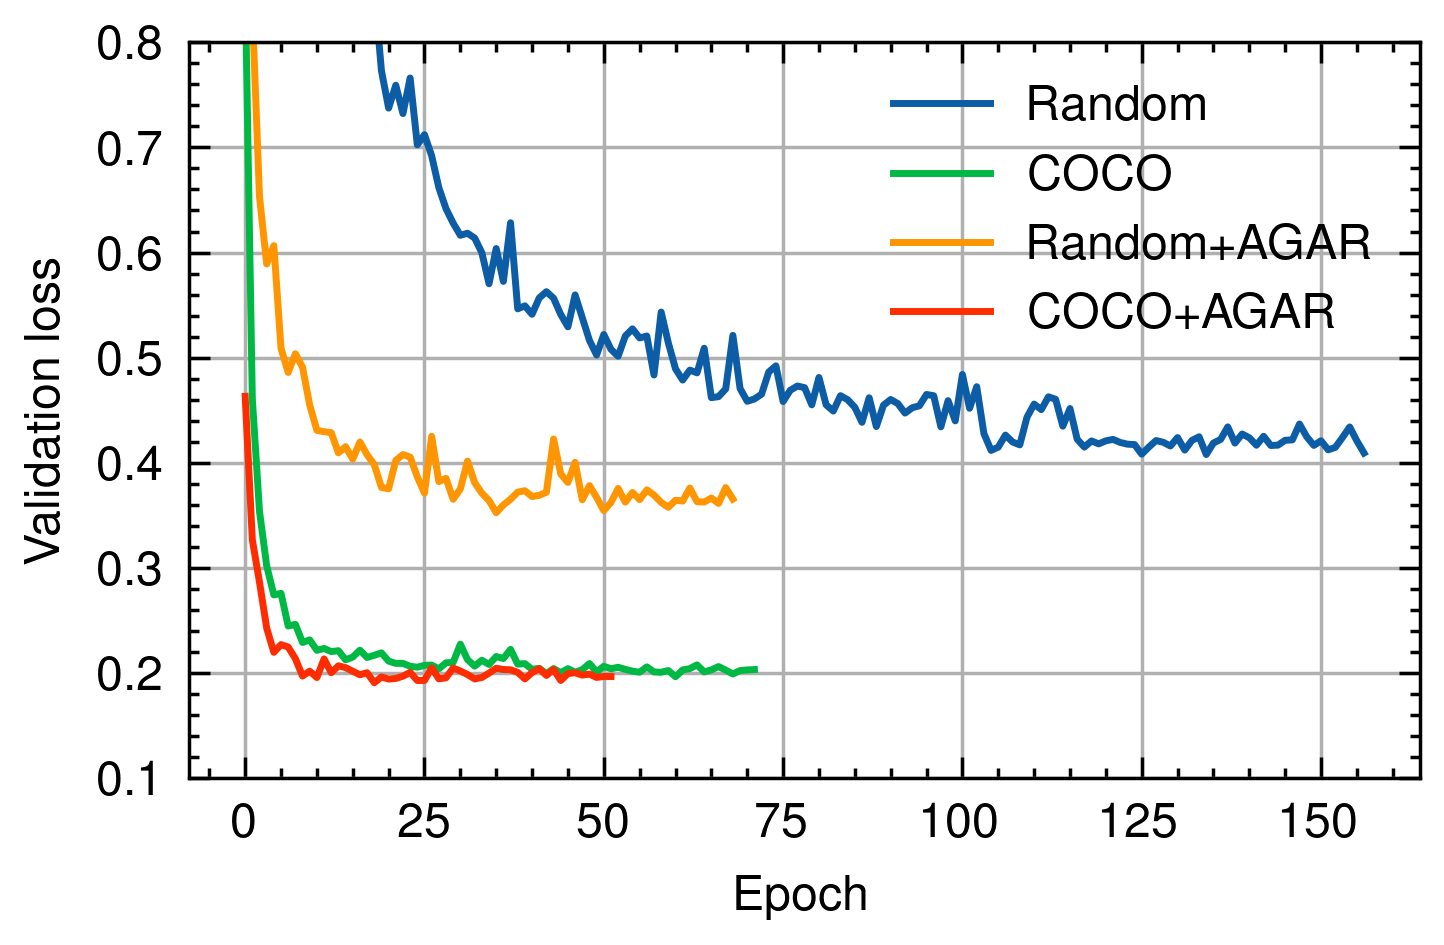
\includegraphics[width=0.65\textwidth]{assets/chart_dataset_comparison_loss}
  \caption{Validation loss plot for different dataset combinations}
  \label{fig:chart_dataset_comparison_loss}
\end{figure}

As visible in Figure \ref{fig:chart_dataset_comparison_loss}, pre-trained models converge much faster. As explained earlier, the learning rate scheduler stops training after validation loss stagnates for some time. For the COCO+AGAR run that happens already after 51 epochs. For runs that use only one of these datasets for pre-training it happens after roughly 70 epochs, while the randomly initialized run takes more than 150 epochs to finish.

\begin{table}[h]
\centering
\begin{tabular}{lcccc}
\hline
 & Epochs & mAP & MAE & sMAPE \\
\hline
Random & 156 & 0.6919 & 9.7 & 0.2492 \\
COCO & 71 & 0.7607 & 6.92 & 0.1842 \\
Random+AGAR & 68 & 0.7065 & 8 & 0.1608 \\
COCO+AGAR & \textbf{51} & \textbf{0.7908} & \textbf{4.64} & \textbf{0.1356} \\
\hline
\end{tabular}
\caption{Comparison of validation metrics for different dataset combinations}
\label{table:datasets_metrics}
\end{table}

\begin{figure}[hbt]
  \centering
  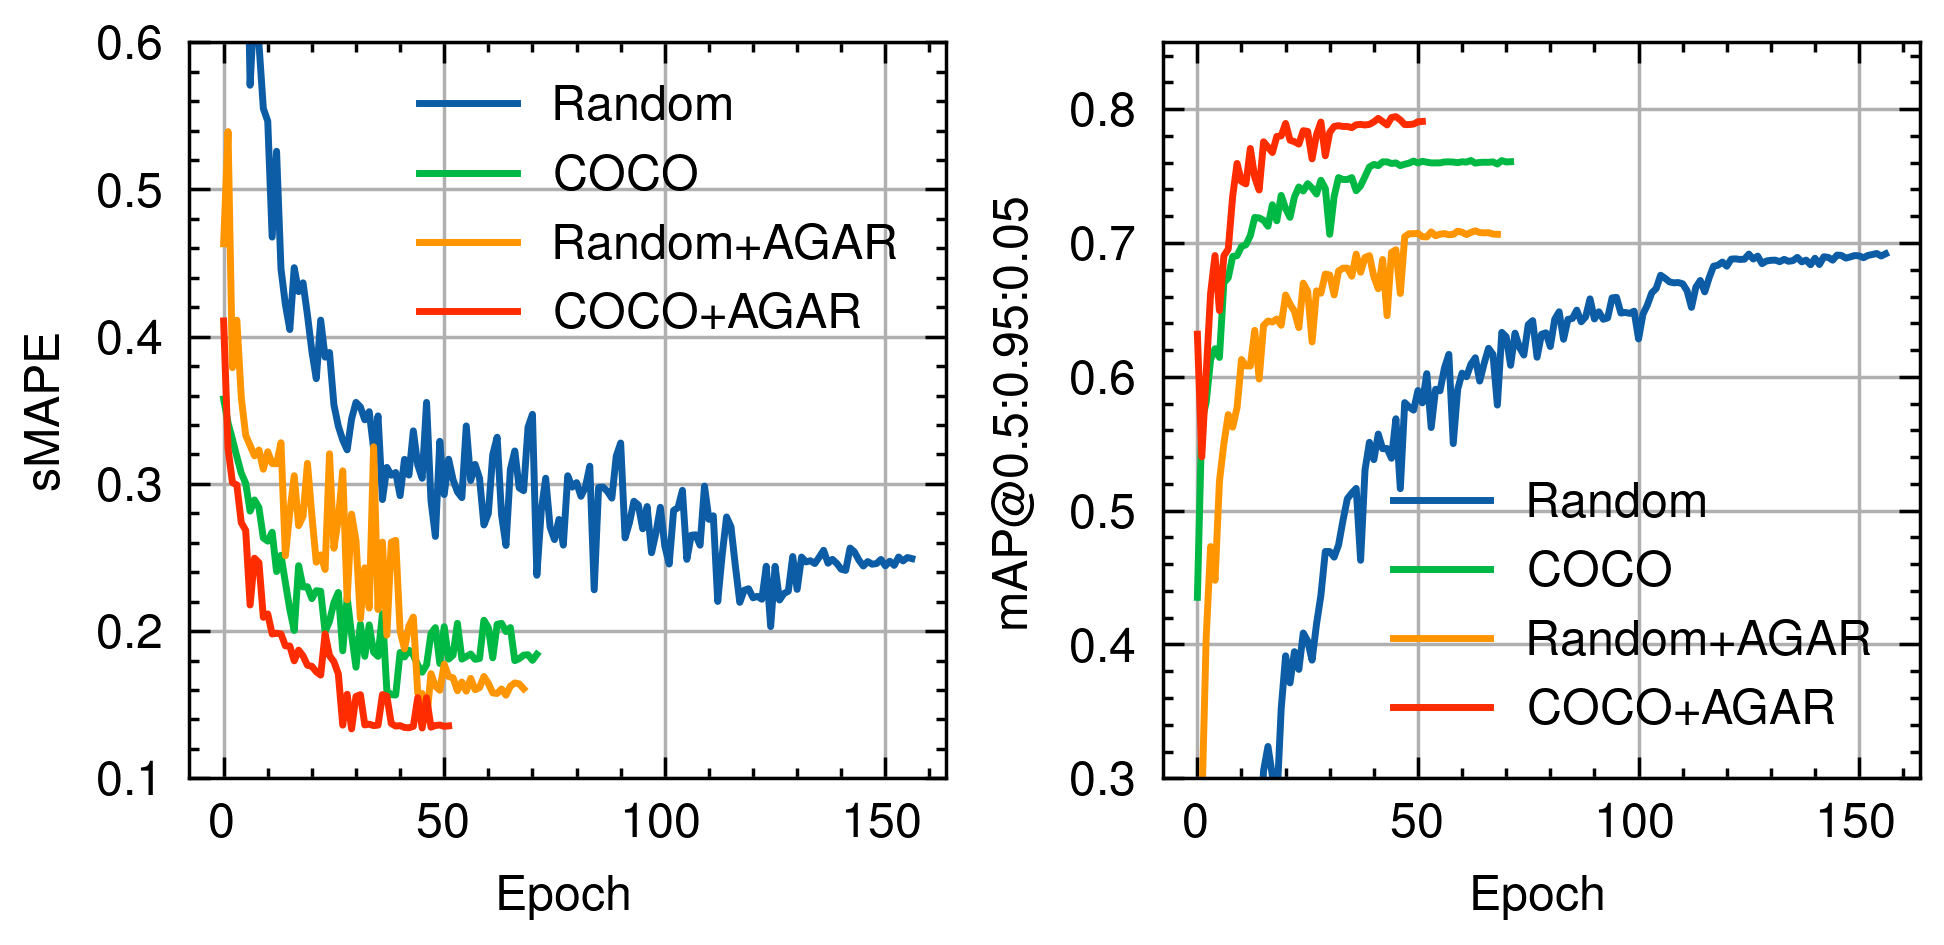
\includegraphics[width=0.8\textwidth]{assets/chart_dataset_comparison}
  \caption{Validation metrics on the photobox validation set for different dataset combinations}
  \label{fig:chart_dataset_comparison_metrics}
\end{figure}

Not only do they converge faster, but as seen in Table \ref{table:datasets_metrics} and Figure \ref{fig:chart_dataset_comparison_metrics}, they also perform better. The combination of COCO+AGAR leads to the highest precision and best counting metrics, needing the fewest epochs for the photobox dataset.

Using pre-trained COCO weights instead of randomly initialized weights seems to have a positive impact on precision, improving it by 9.94\%. Using the AGAR dataset for pre-training seems to have an especially positive impact on the primary counting metric sMAPE, improving it by 35.5\%. Combining these two datasets for pre-training leads to an improvement in precision by 14.3\% and sMAPE by 45.6\%, while only having to train for approximately one third of the epochs.

\begin{table}[ht]
\centering
\caption{Comparison of detections for the different runs}
\label{tab:dataset_comparison_images}
\begin{tabular}{cccc}
\hline
Image & Ground Truth & Random & COCO+AGAR \\ \hline
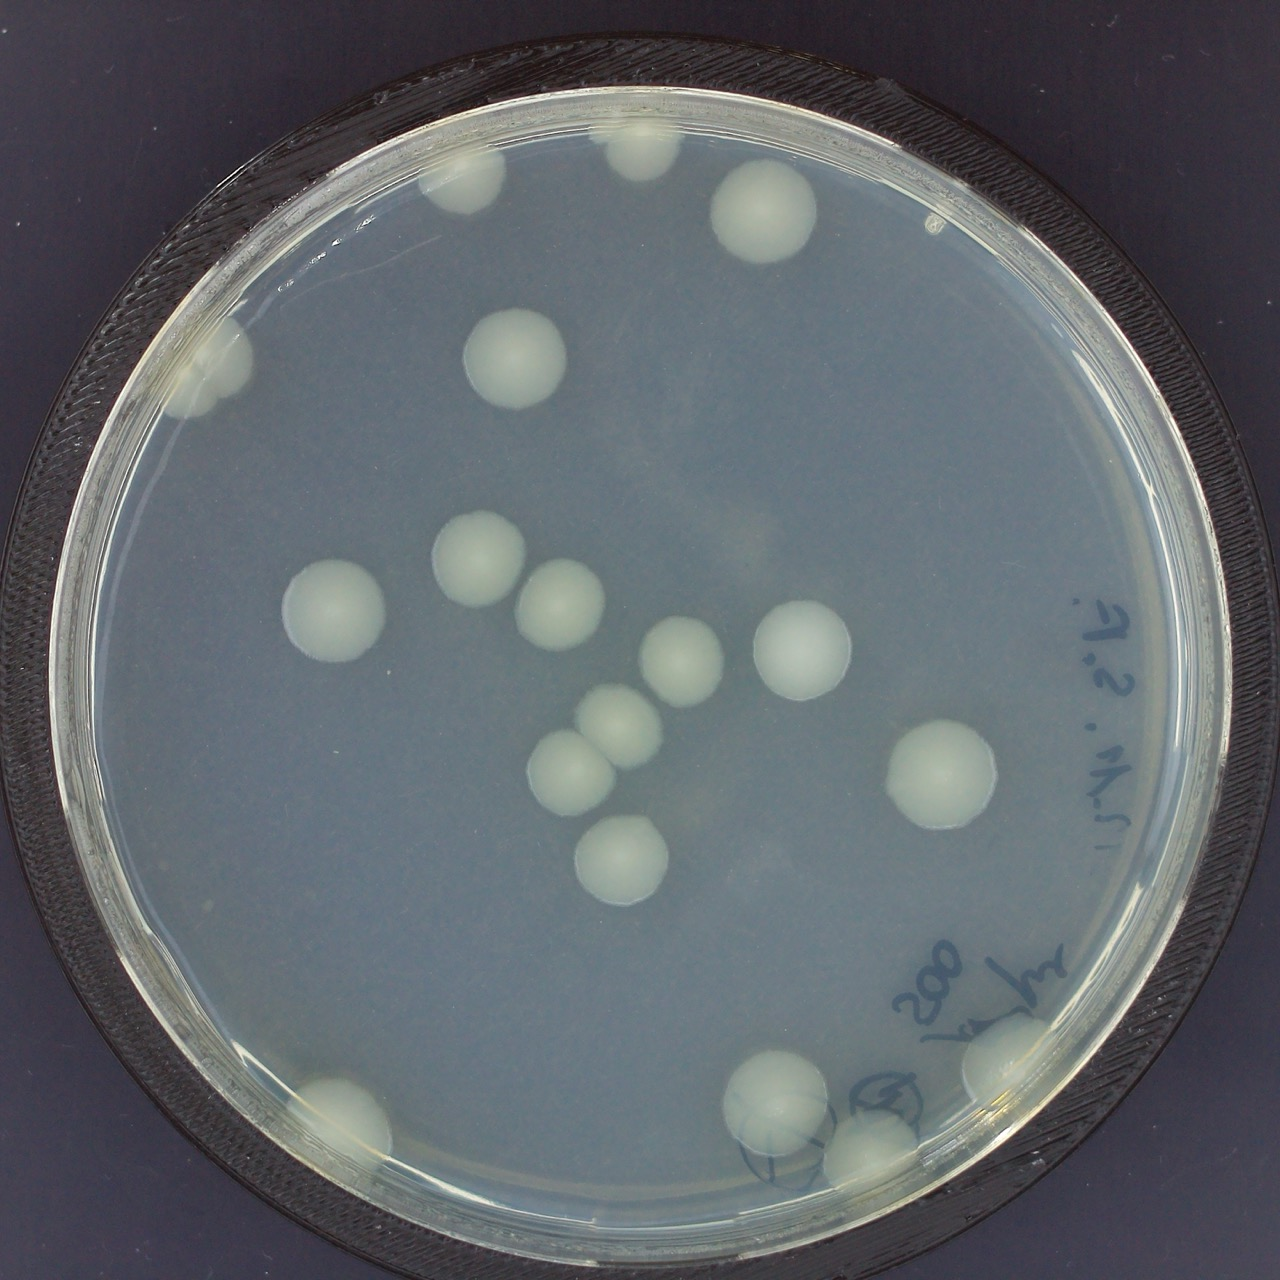
\includegraphics[width=0.2\textwidth]{assets/Y_500µl_2_default_ gvpcagar_default_15122023144938} & 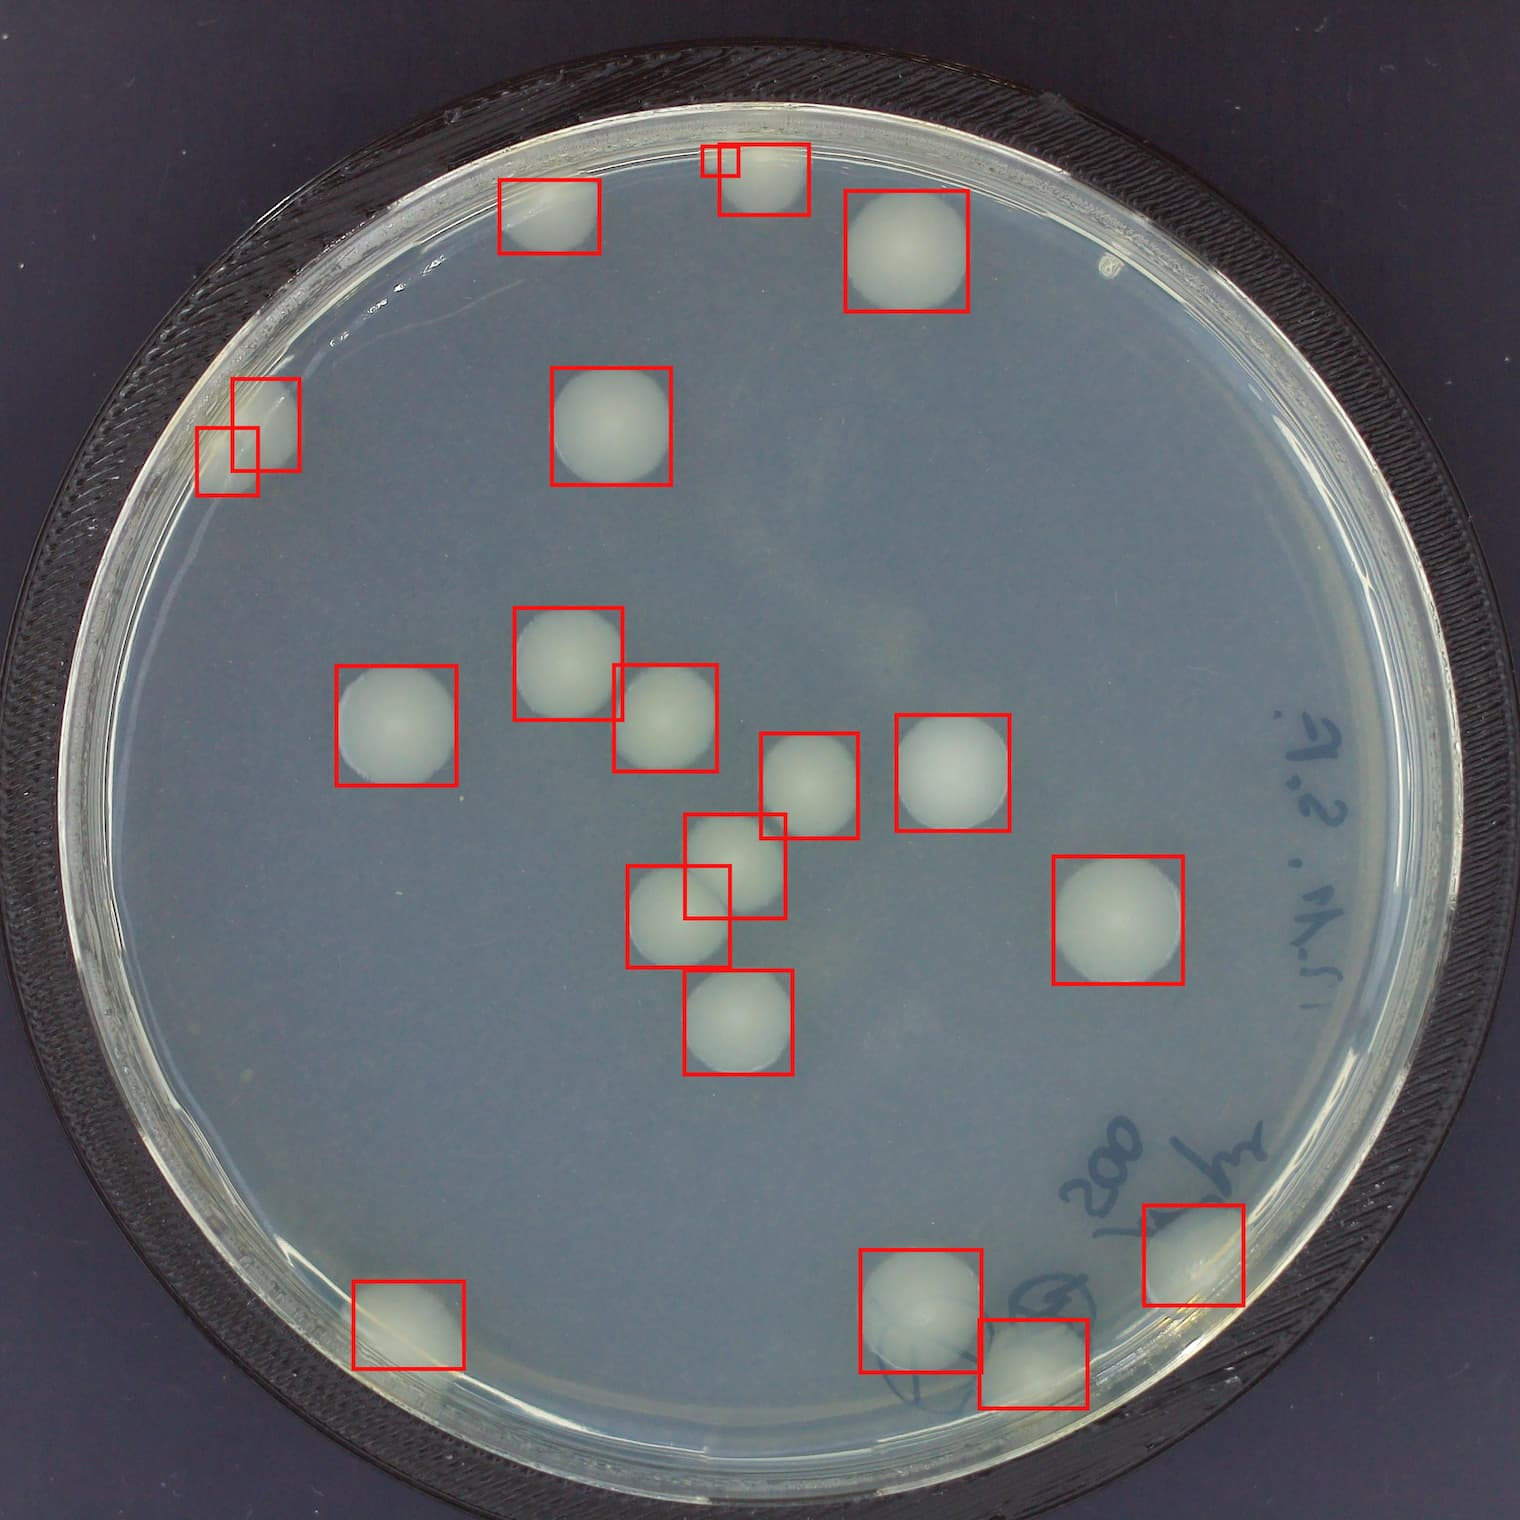
\includegraphics[width=0.2\textwidth]{assets/gt_Y_500µl_2_default_ gvpcagar_default_15122023144938} & 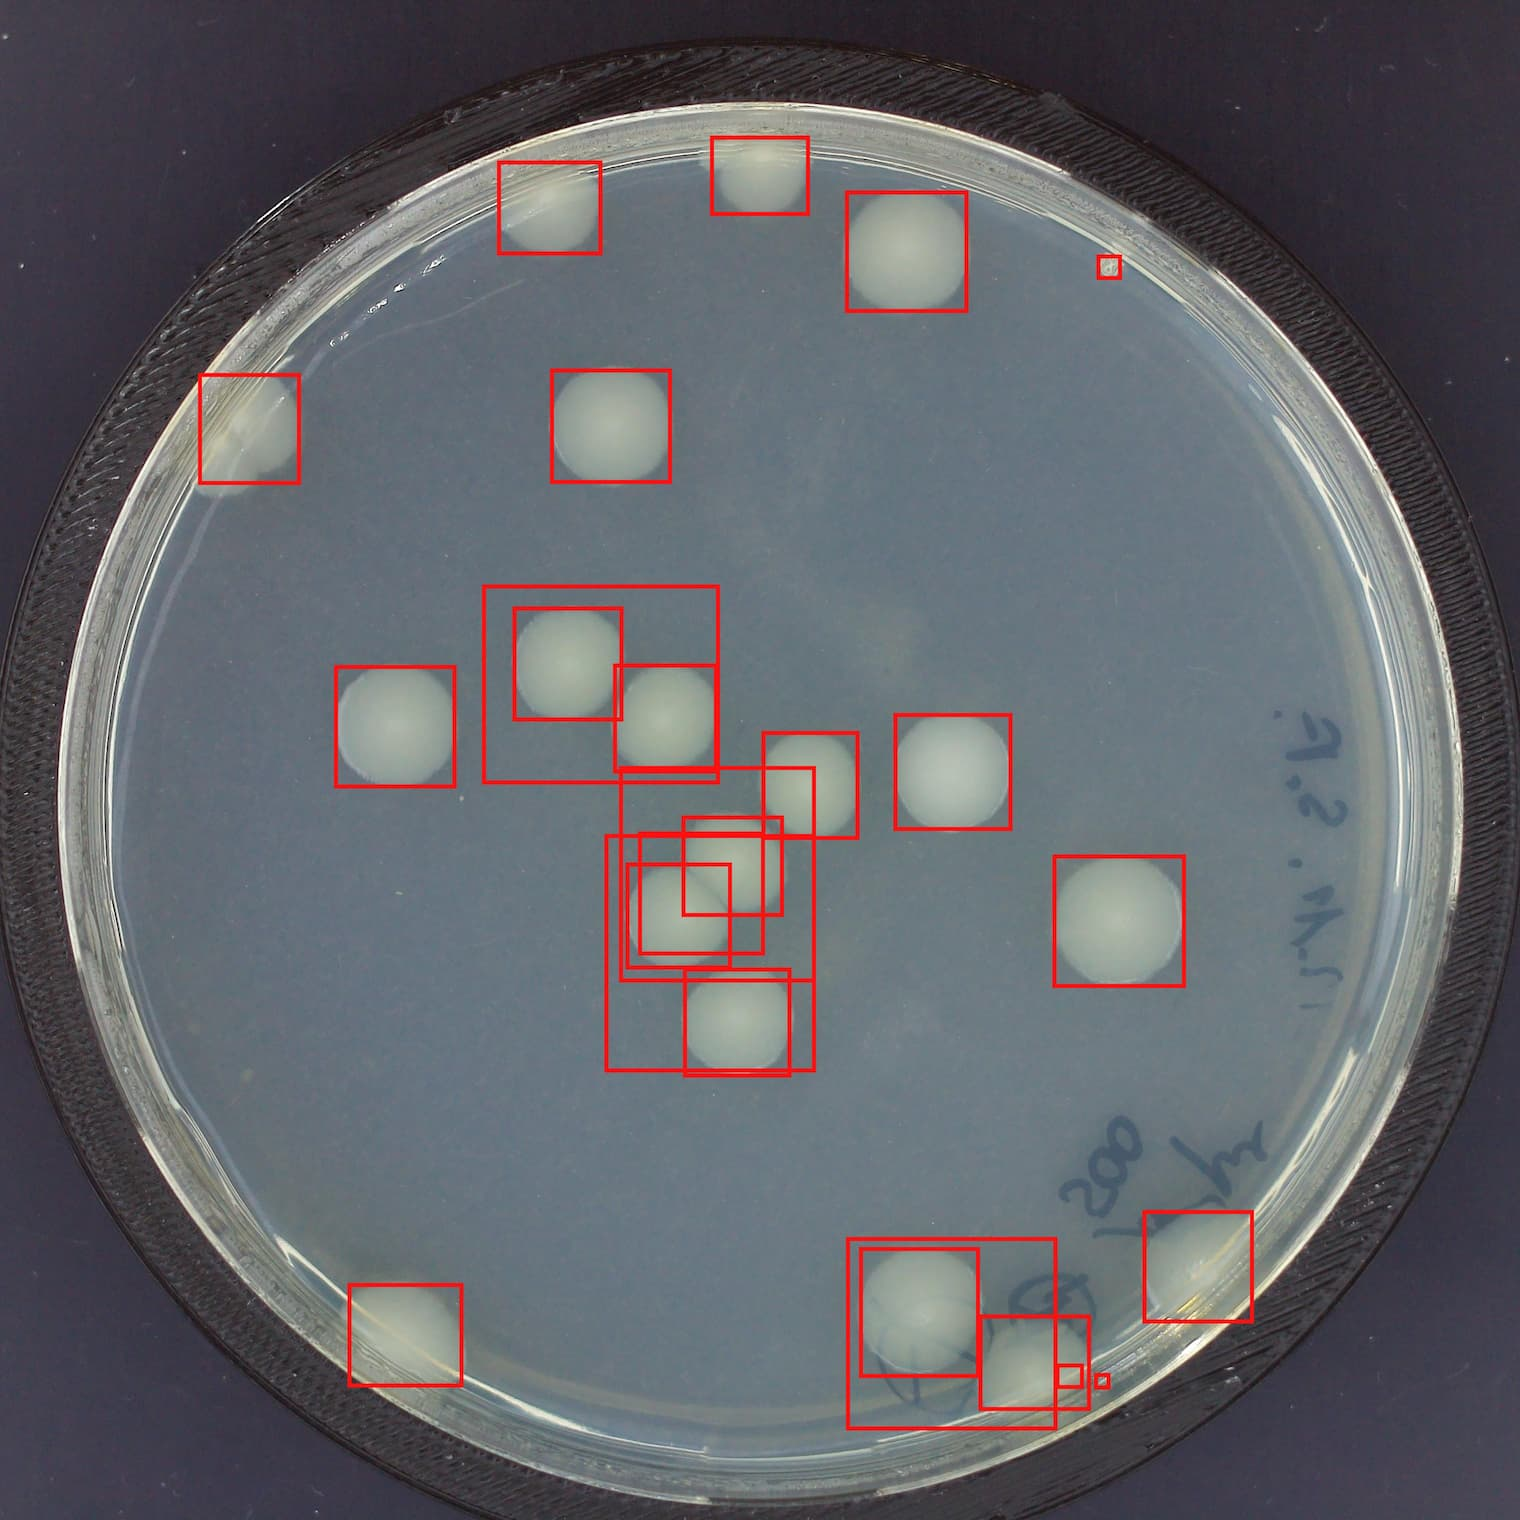
\includegraphics[width=0.2\textwidth]{assets/pred_Y_500µl_2_default_ gvpcagar_default_15122023144938} & 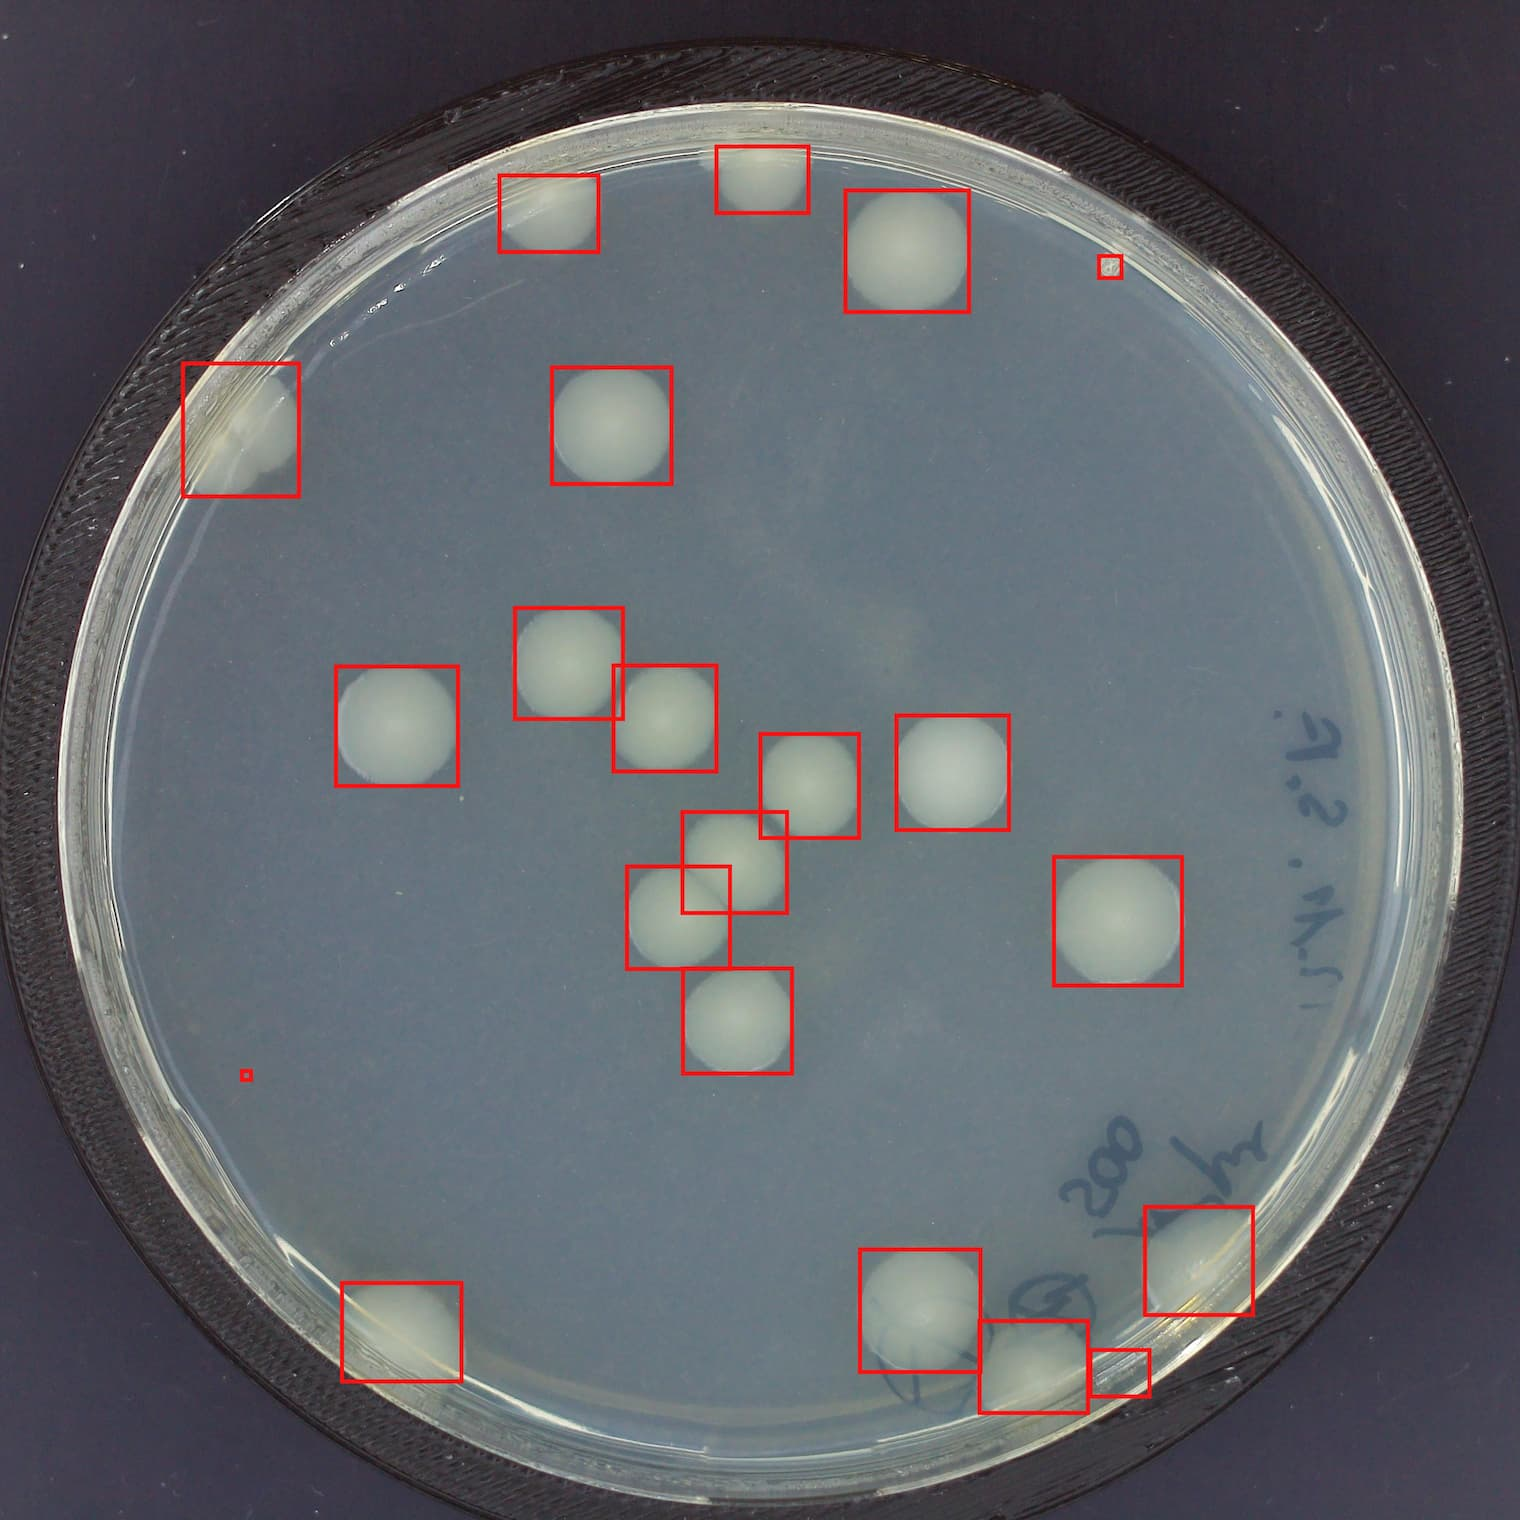
\includegraphics[width=0.2\textwidth]{assets/pt_pred_Y_500µl_2_default_ gvpcagar_default_15122023144938} \\
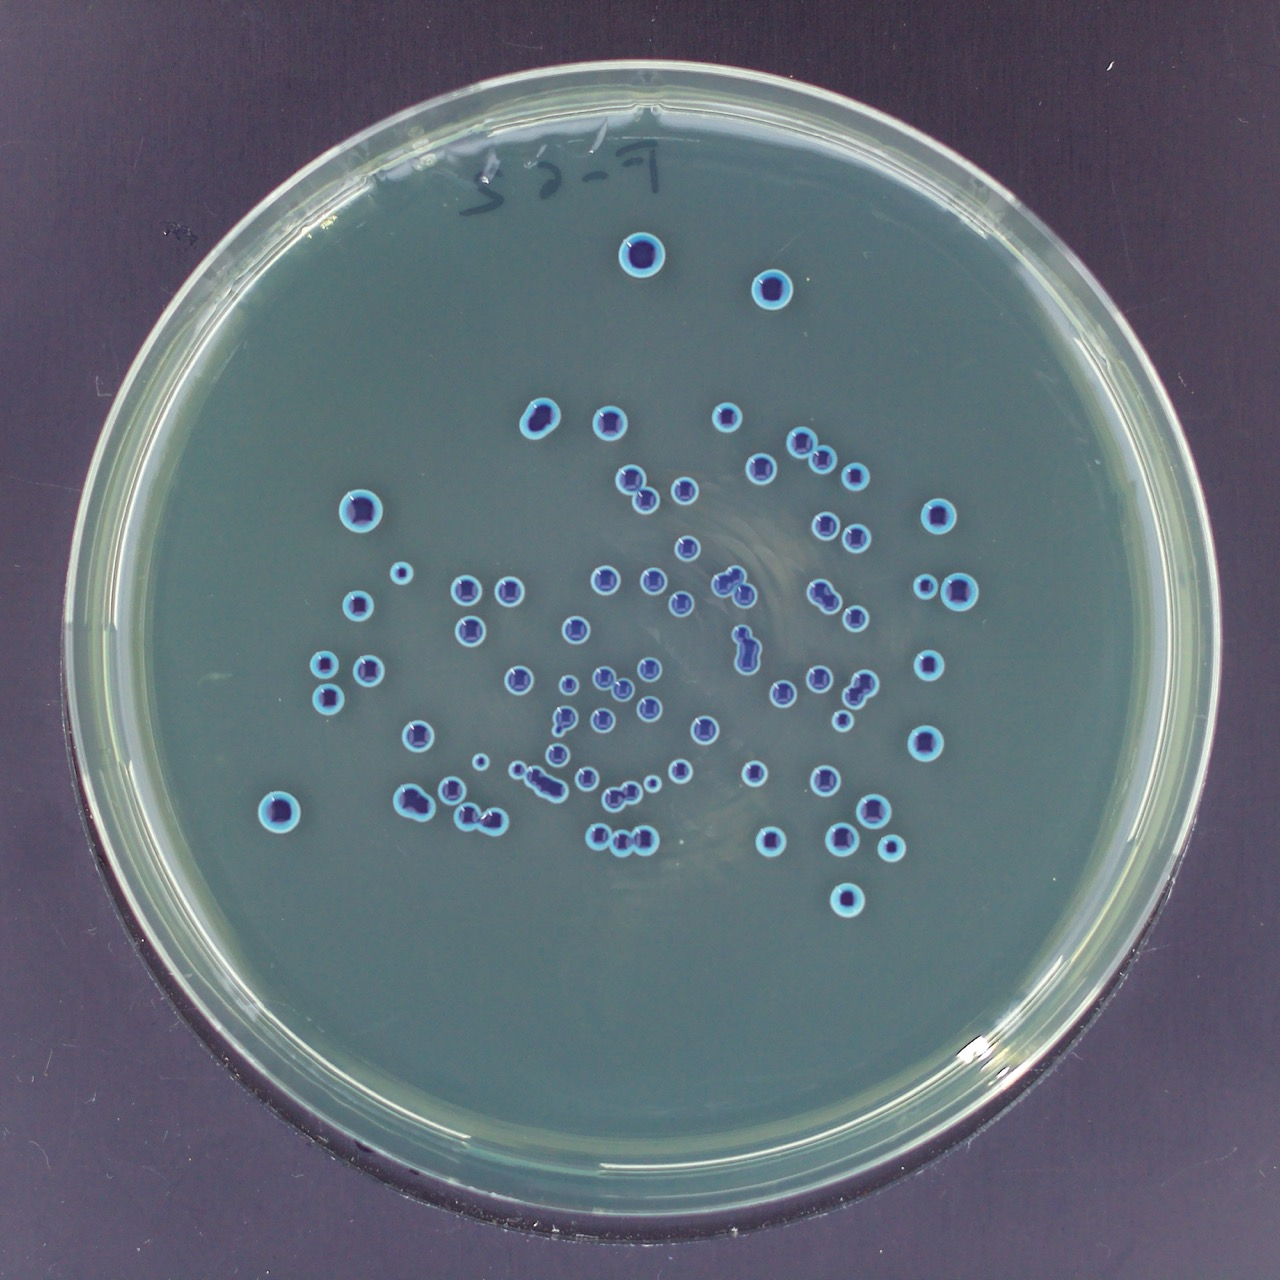
\includegraphics[width=0.2\textwidth]{assets/default_mmrsbpb_default_19012024141840} & 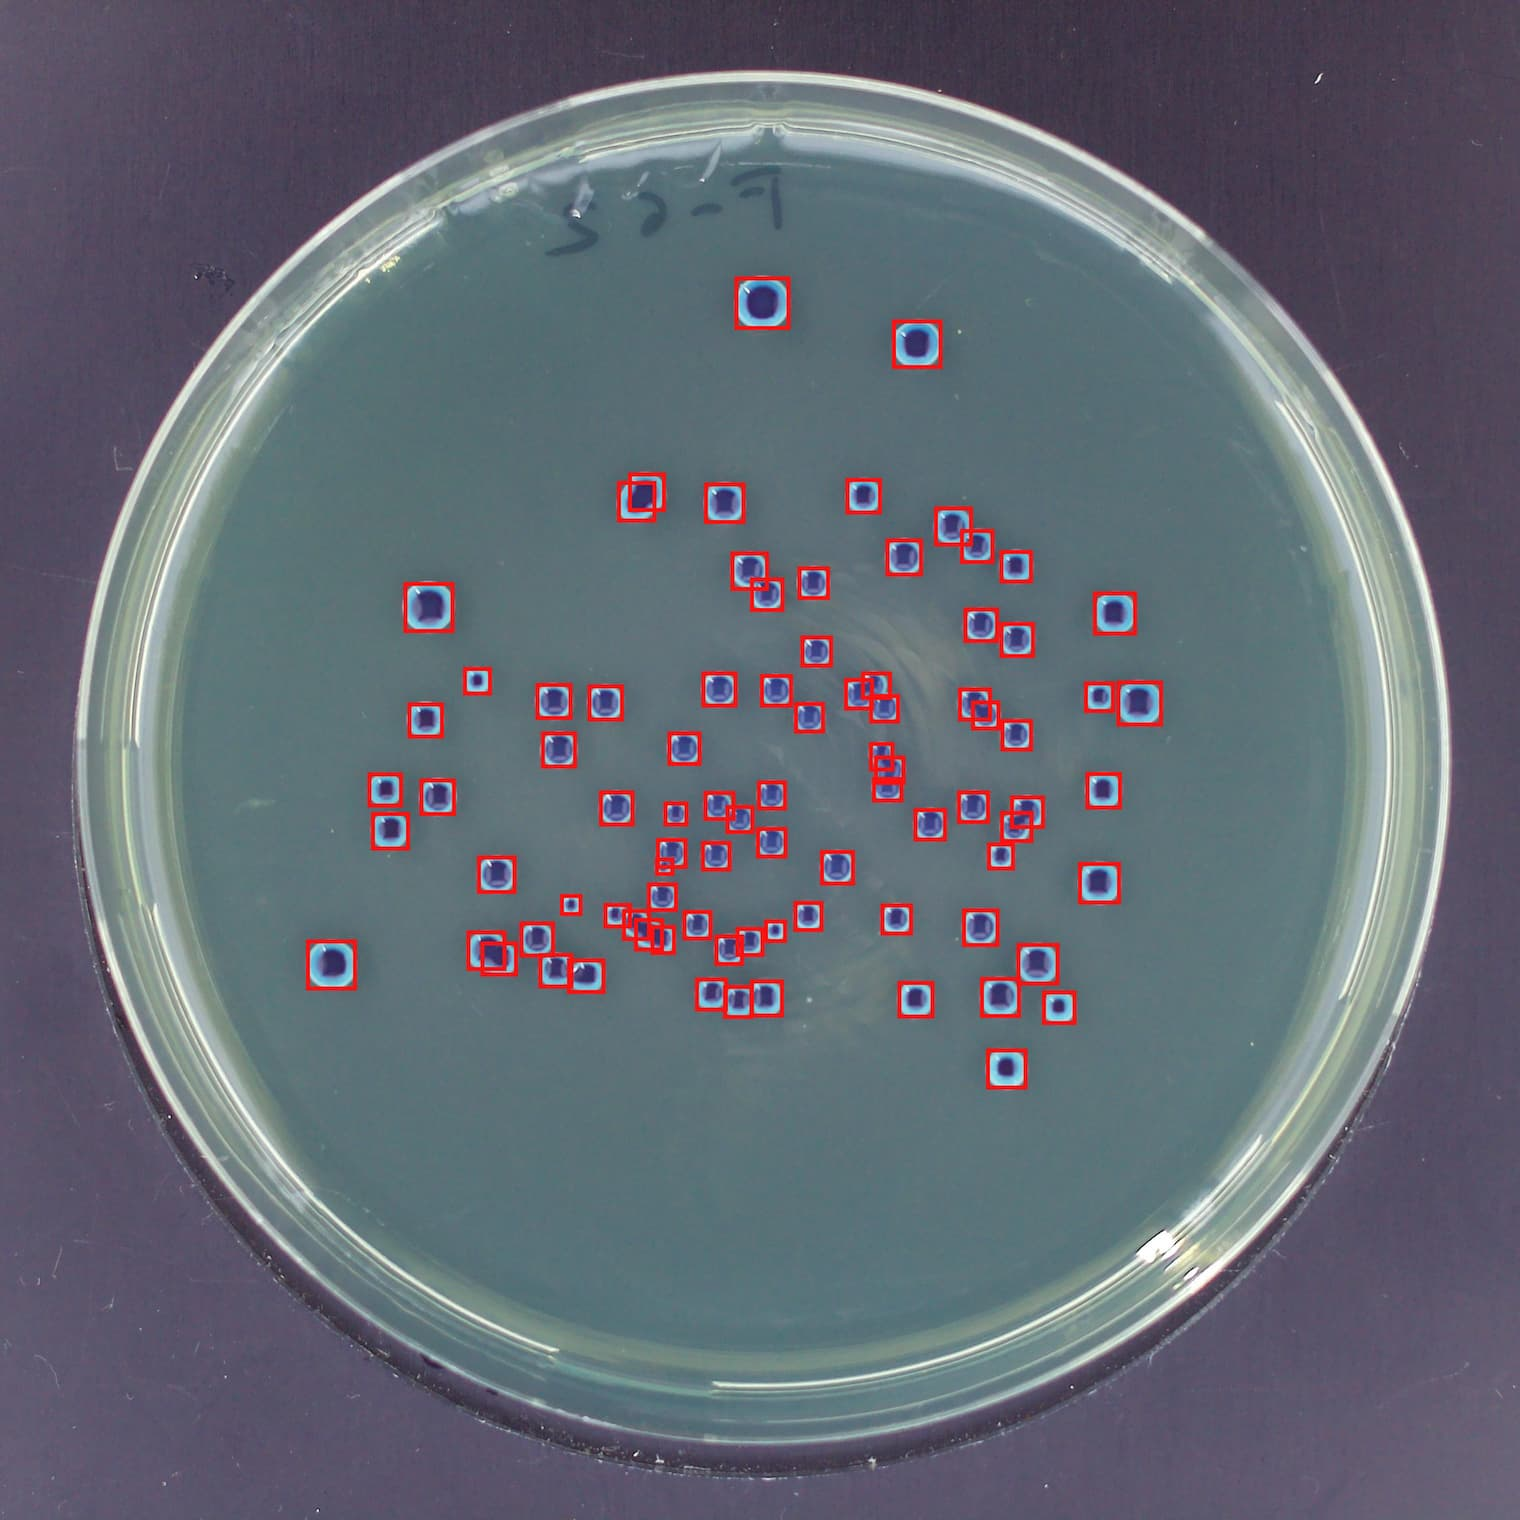
\includegraphics[width=0.2\textwidth]{assets/gt_default_mmrsbpb_default_19012024141840} & 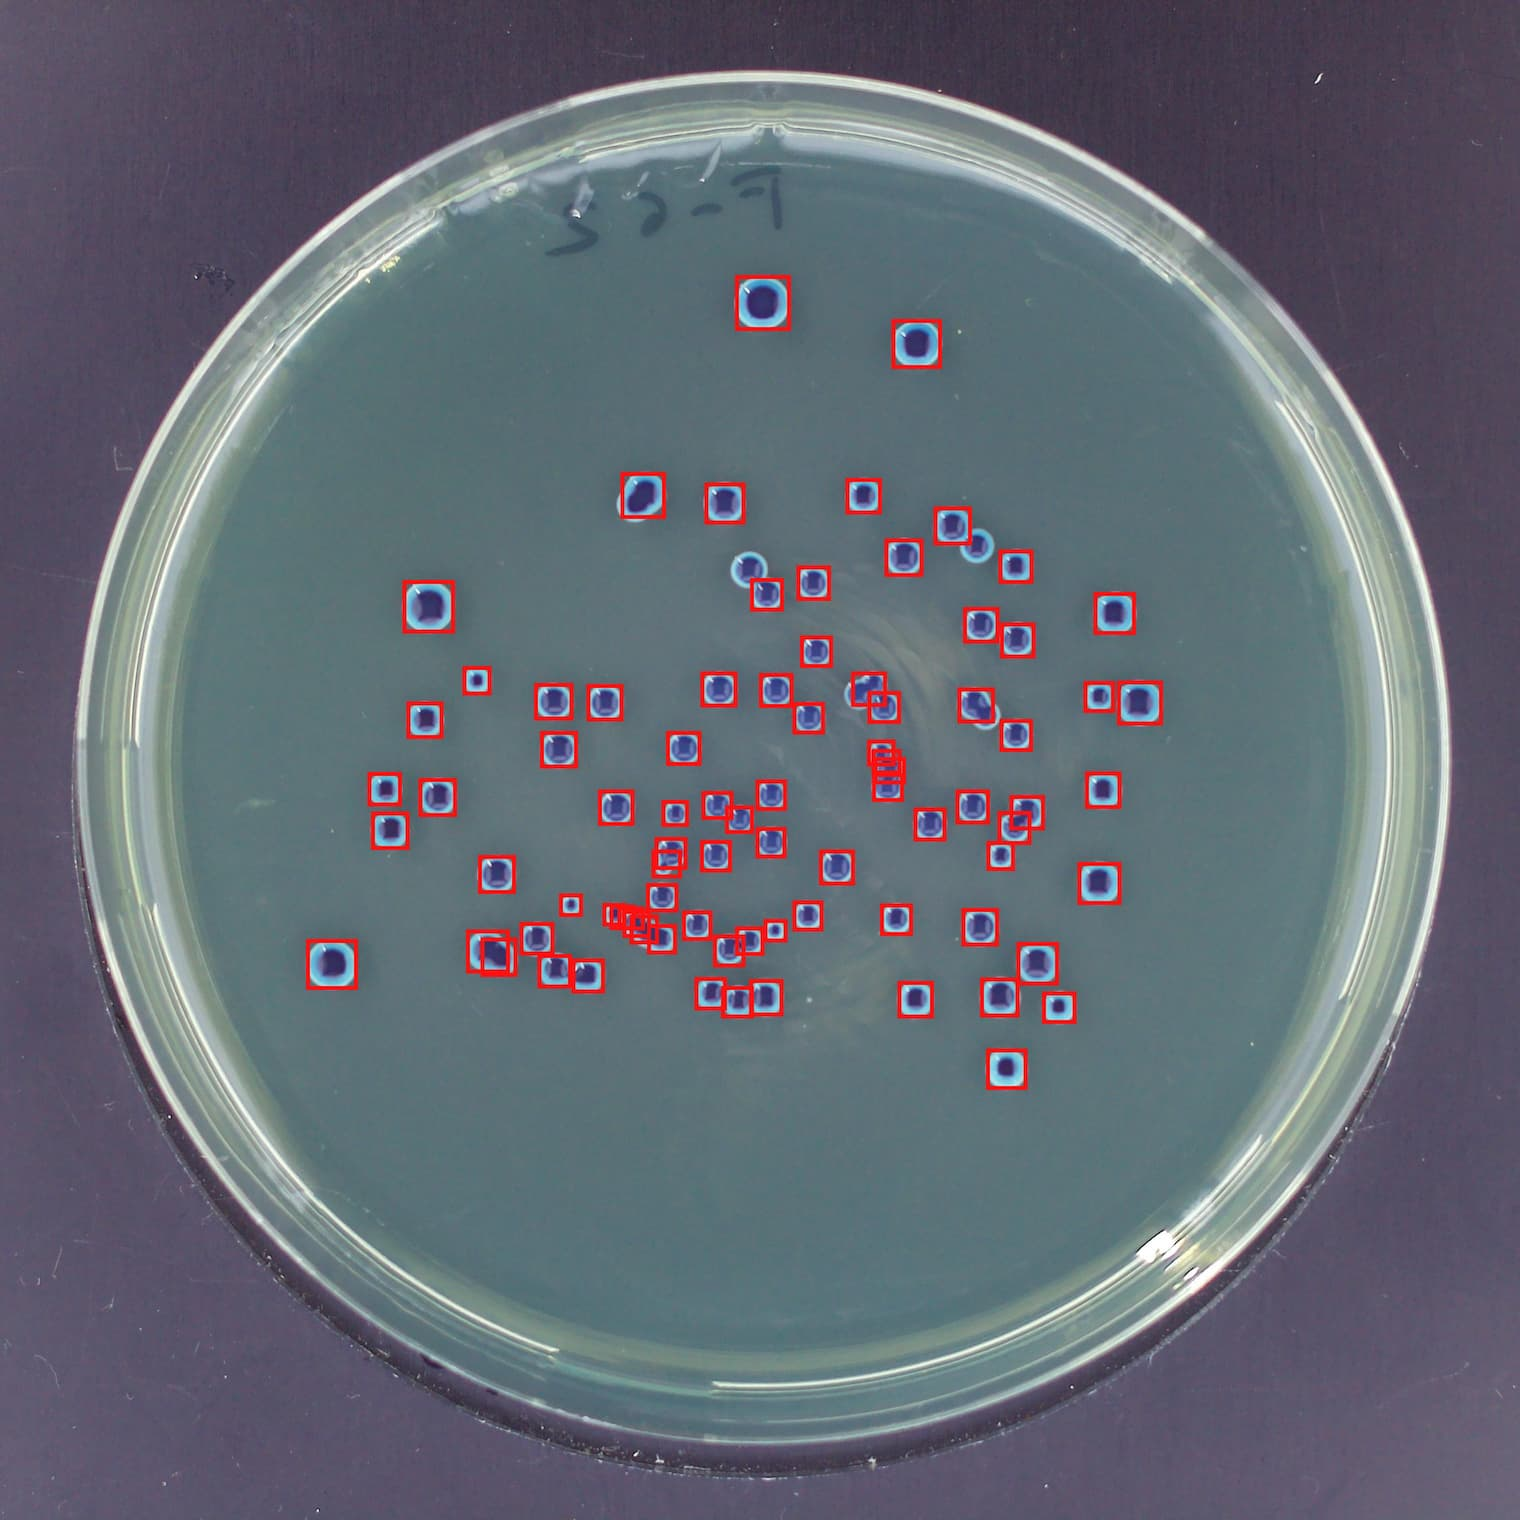
\includegraphics[width=0.2\textwidth]{assets/pred_default_mmrsbpb_default_19012024141840} & 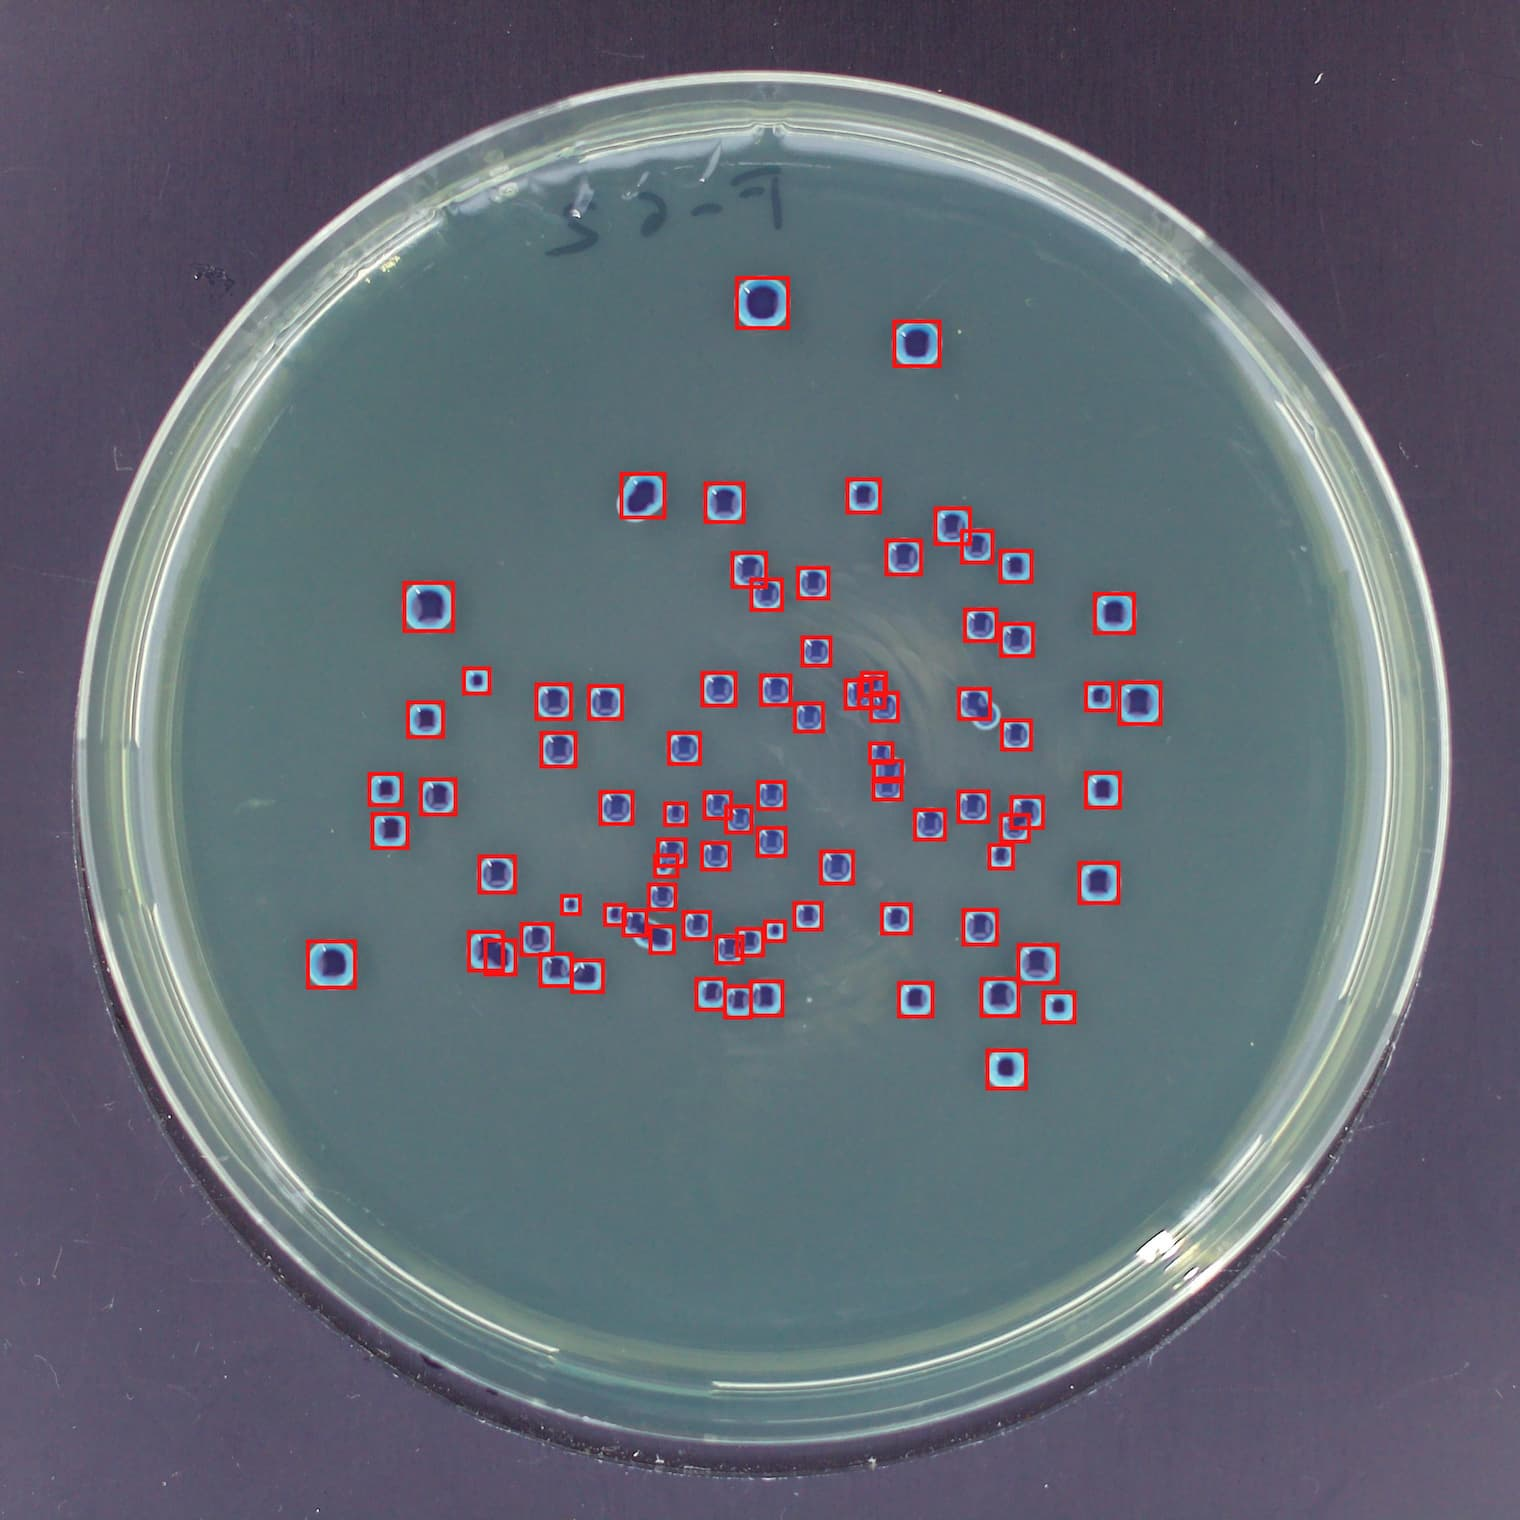
\includegraphics[width=0.2\textwidth]{assets/pt_pred_default_mmrsbpb_default_19012024141840}  \\ 
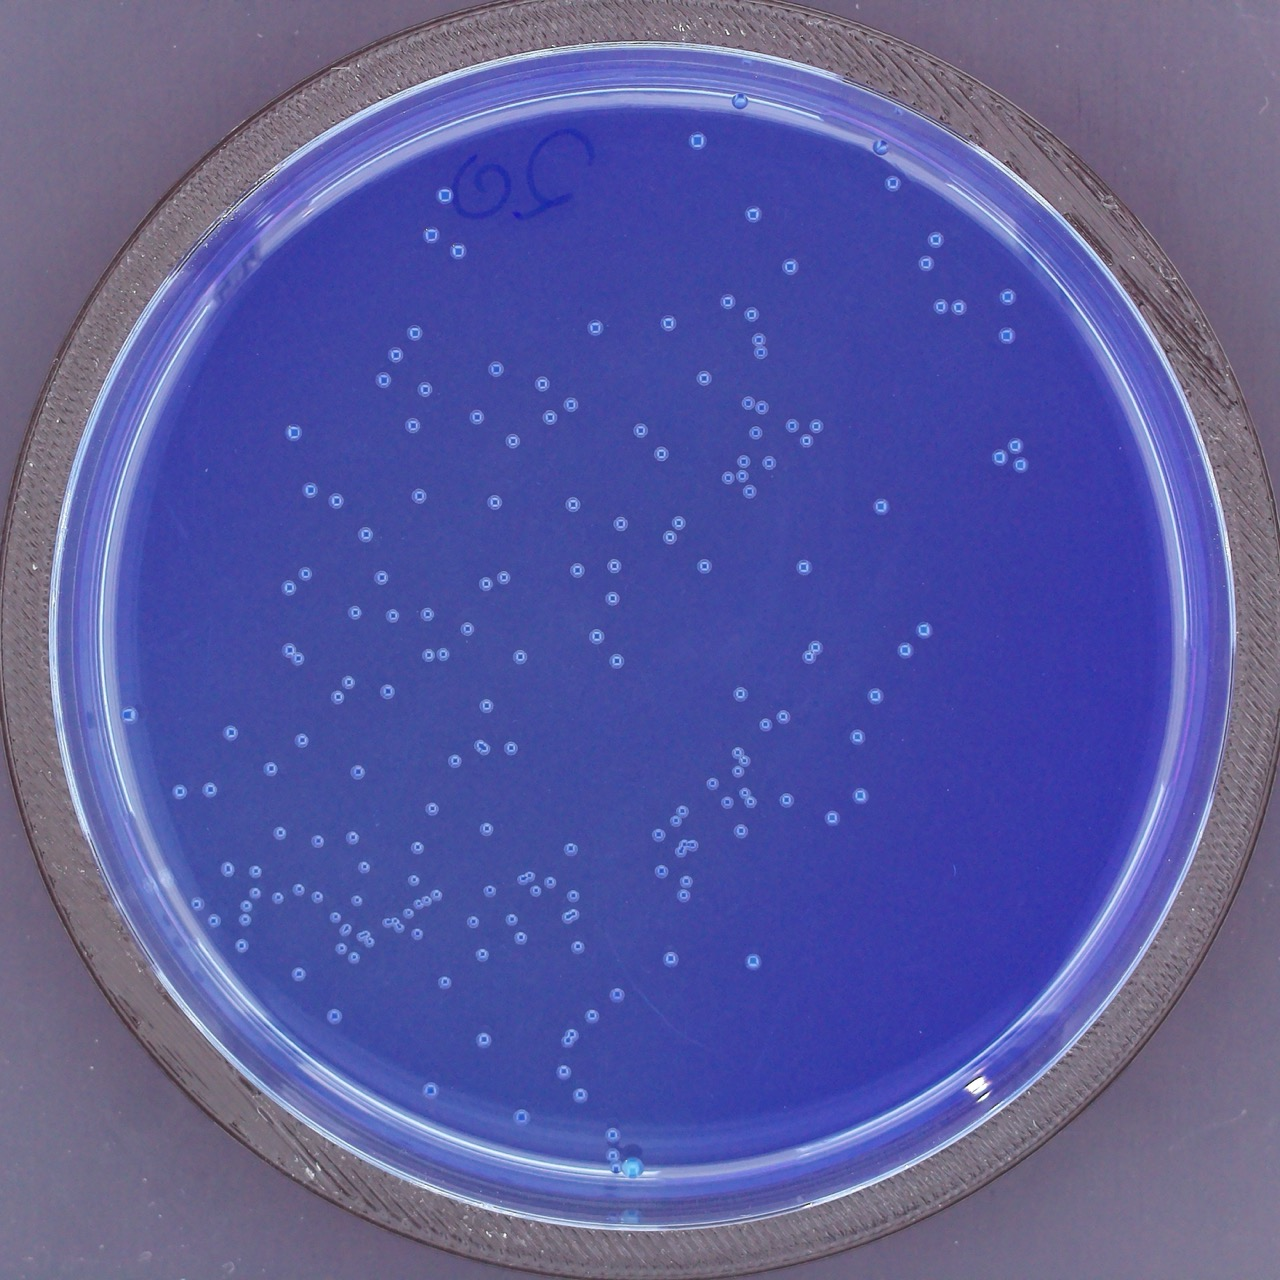
\includegraphics[width=0.2\textwidth]{assets/rod_lentilactobacillus_buchneri_20_default_mmrsbpb_3_07102022120738} & 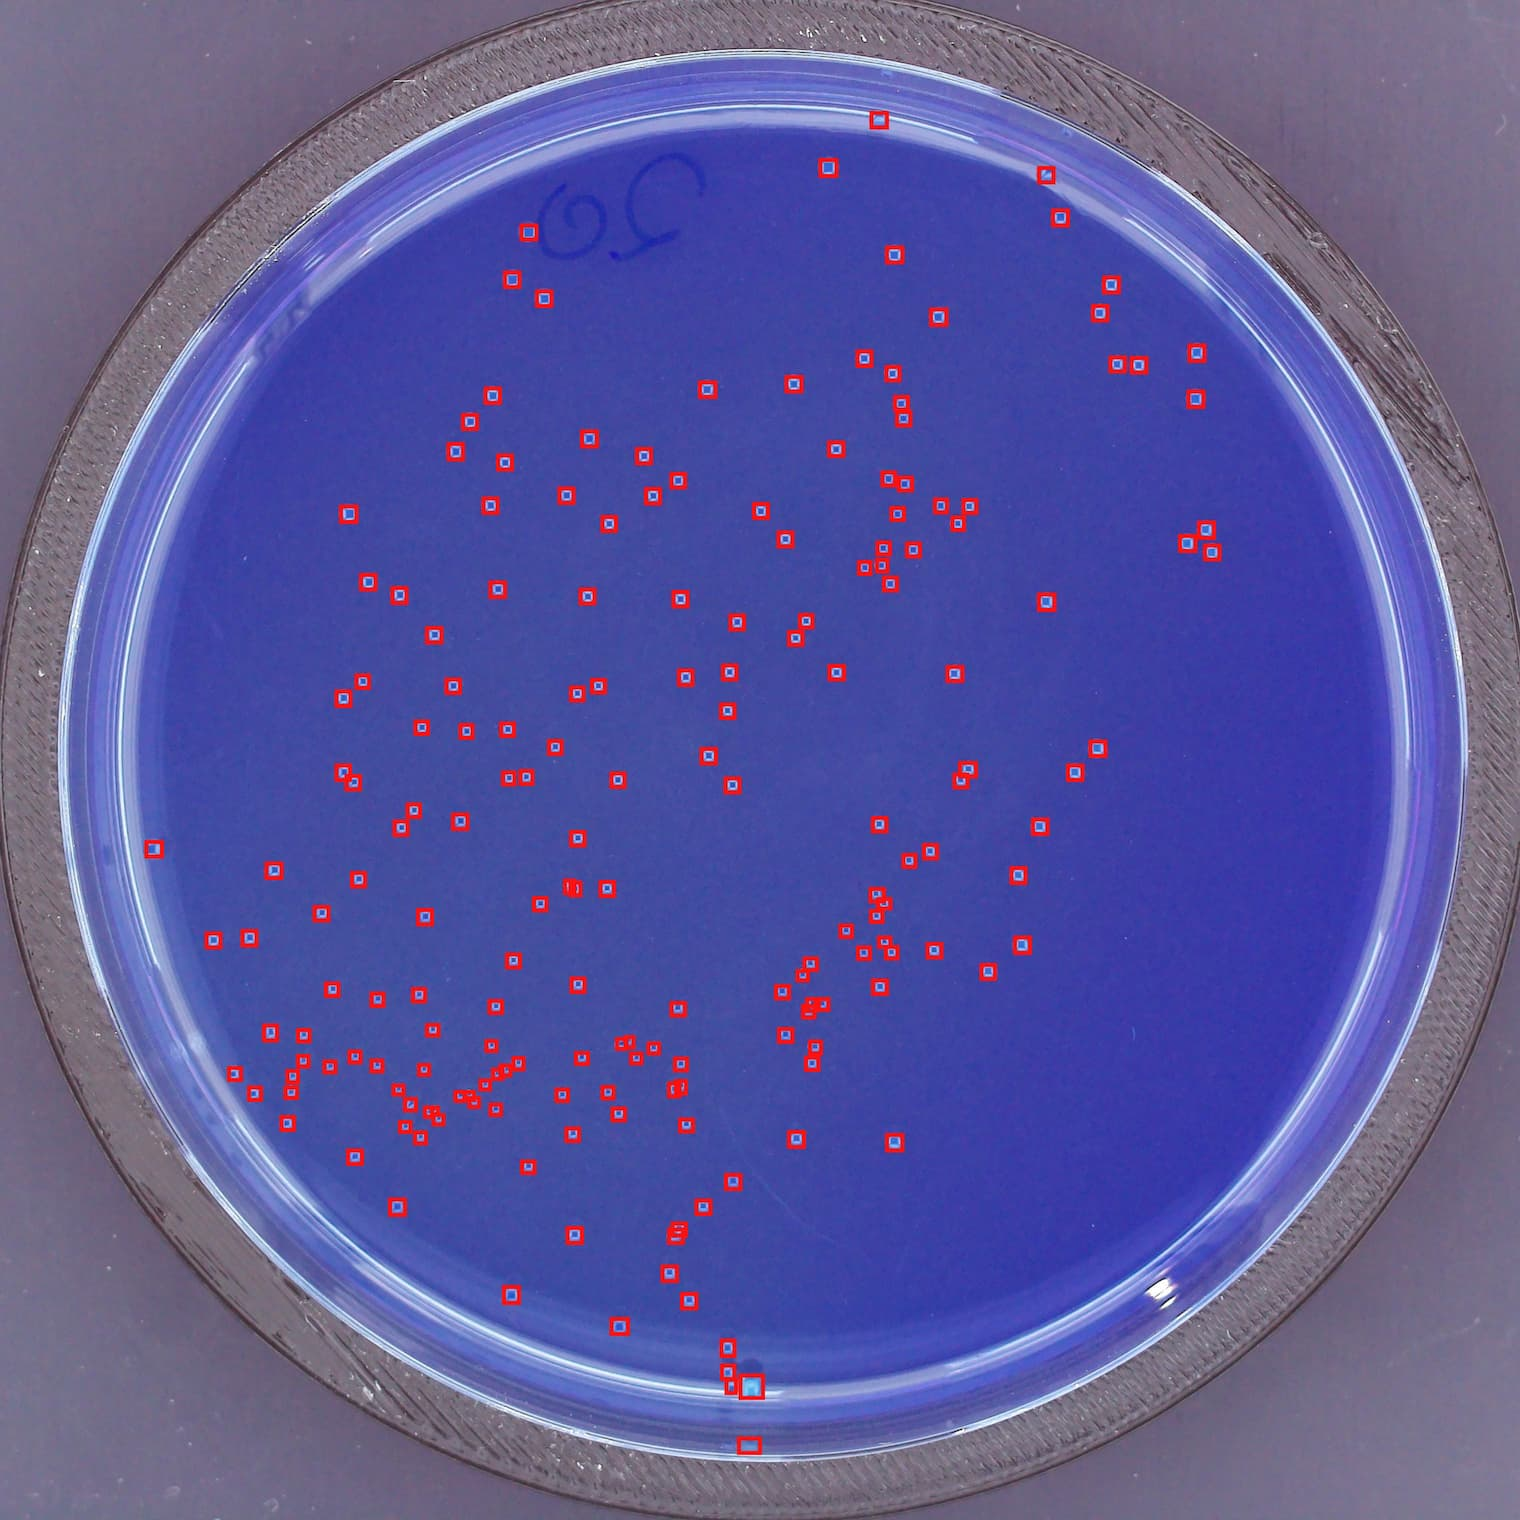
\includegraphics[width=0.2\textwidth]{assets/gt_rod_lentilactobacillus_buchneri_20_default_mmrsbpb_3_07102022120738} & 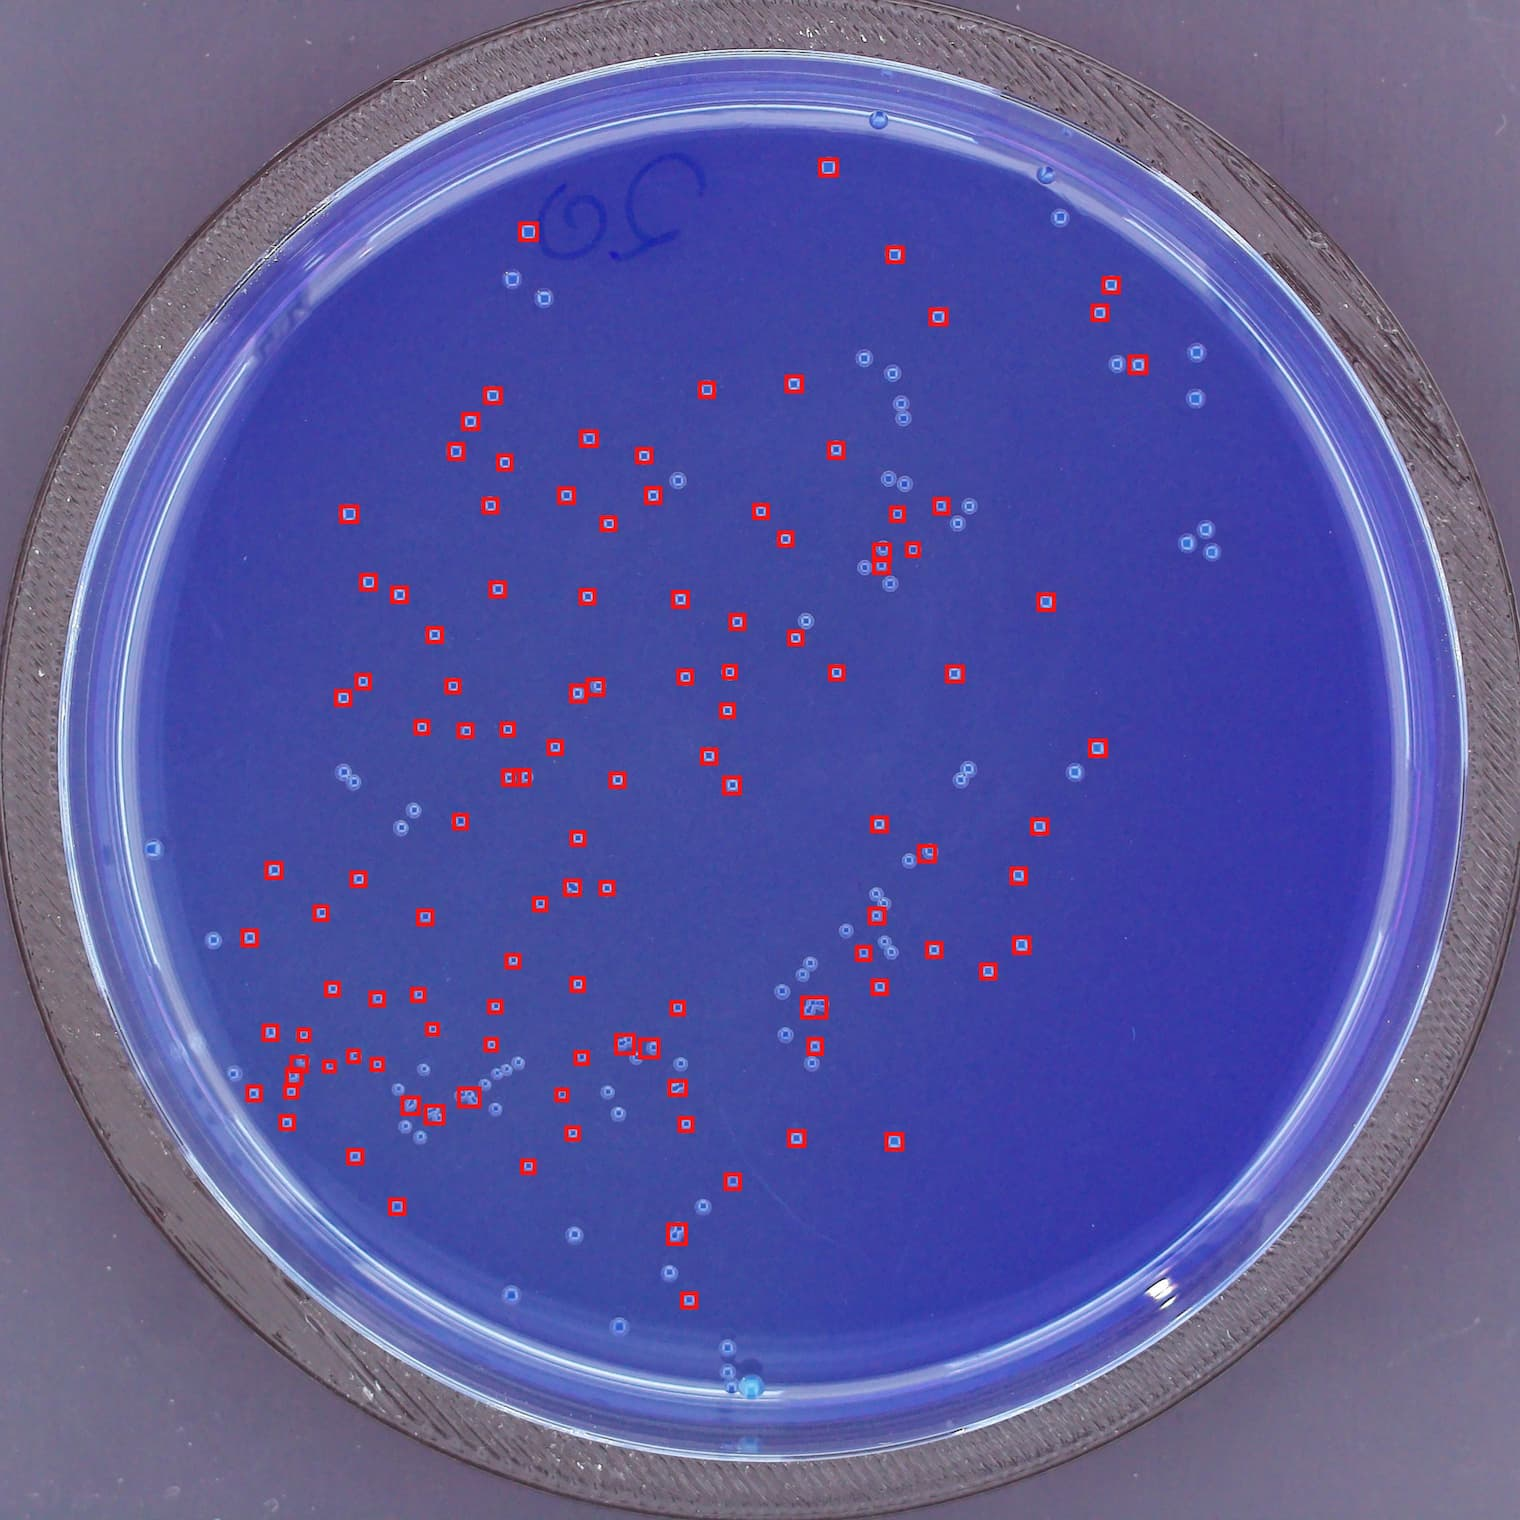
\includegraphics[width=0.2\textwidth]{assets/pred_rod_lentilactobacillus_buchneri_20_default_mmrsbpb_3_07102022120738} & 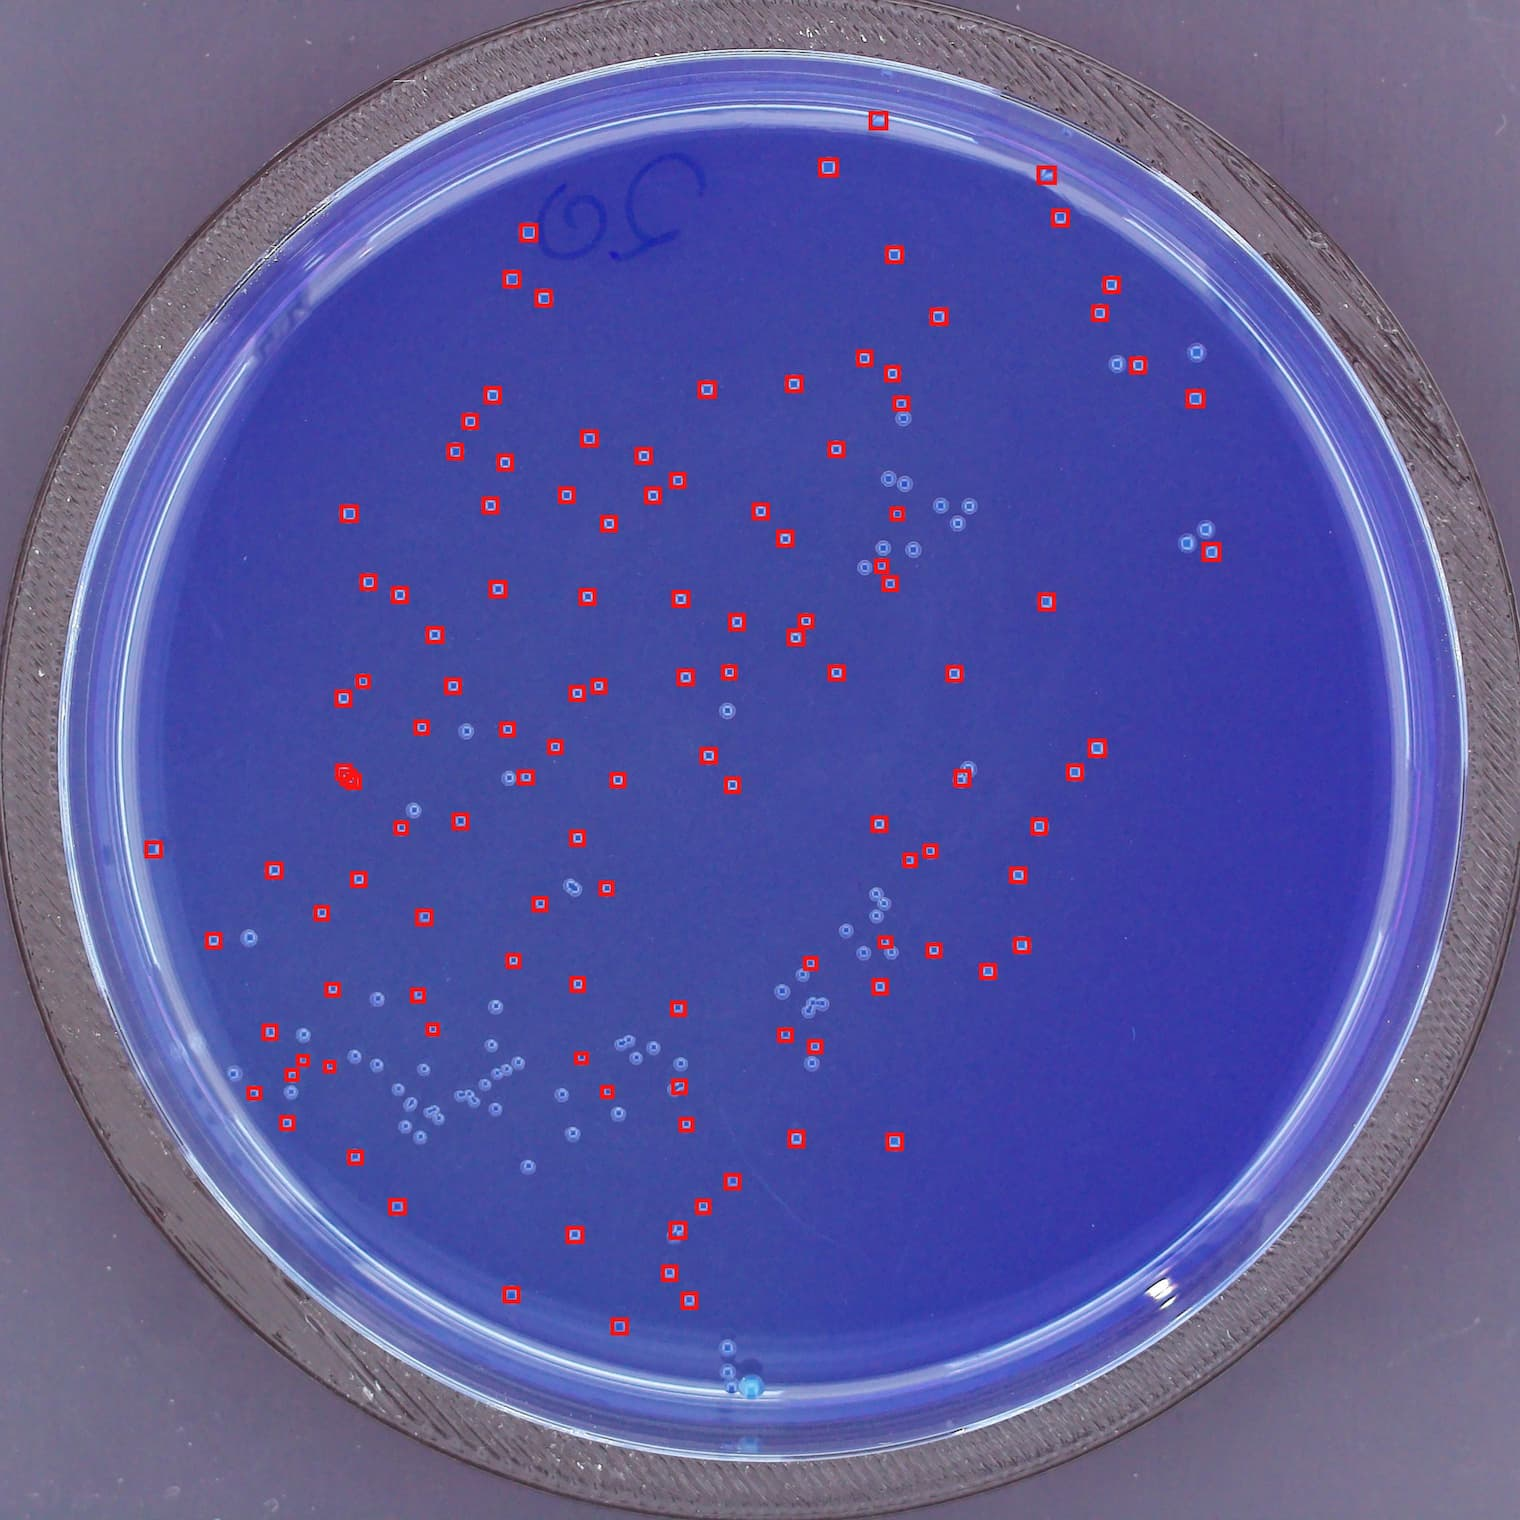
\includegraphics[width=0.2\textwidth]{assets/pt_pred_rod_lentilactobacillus_buchneri_20_default_mmrsbpb_3_07102022120738} \\ 
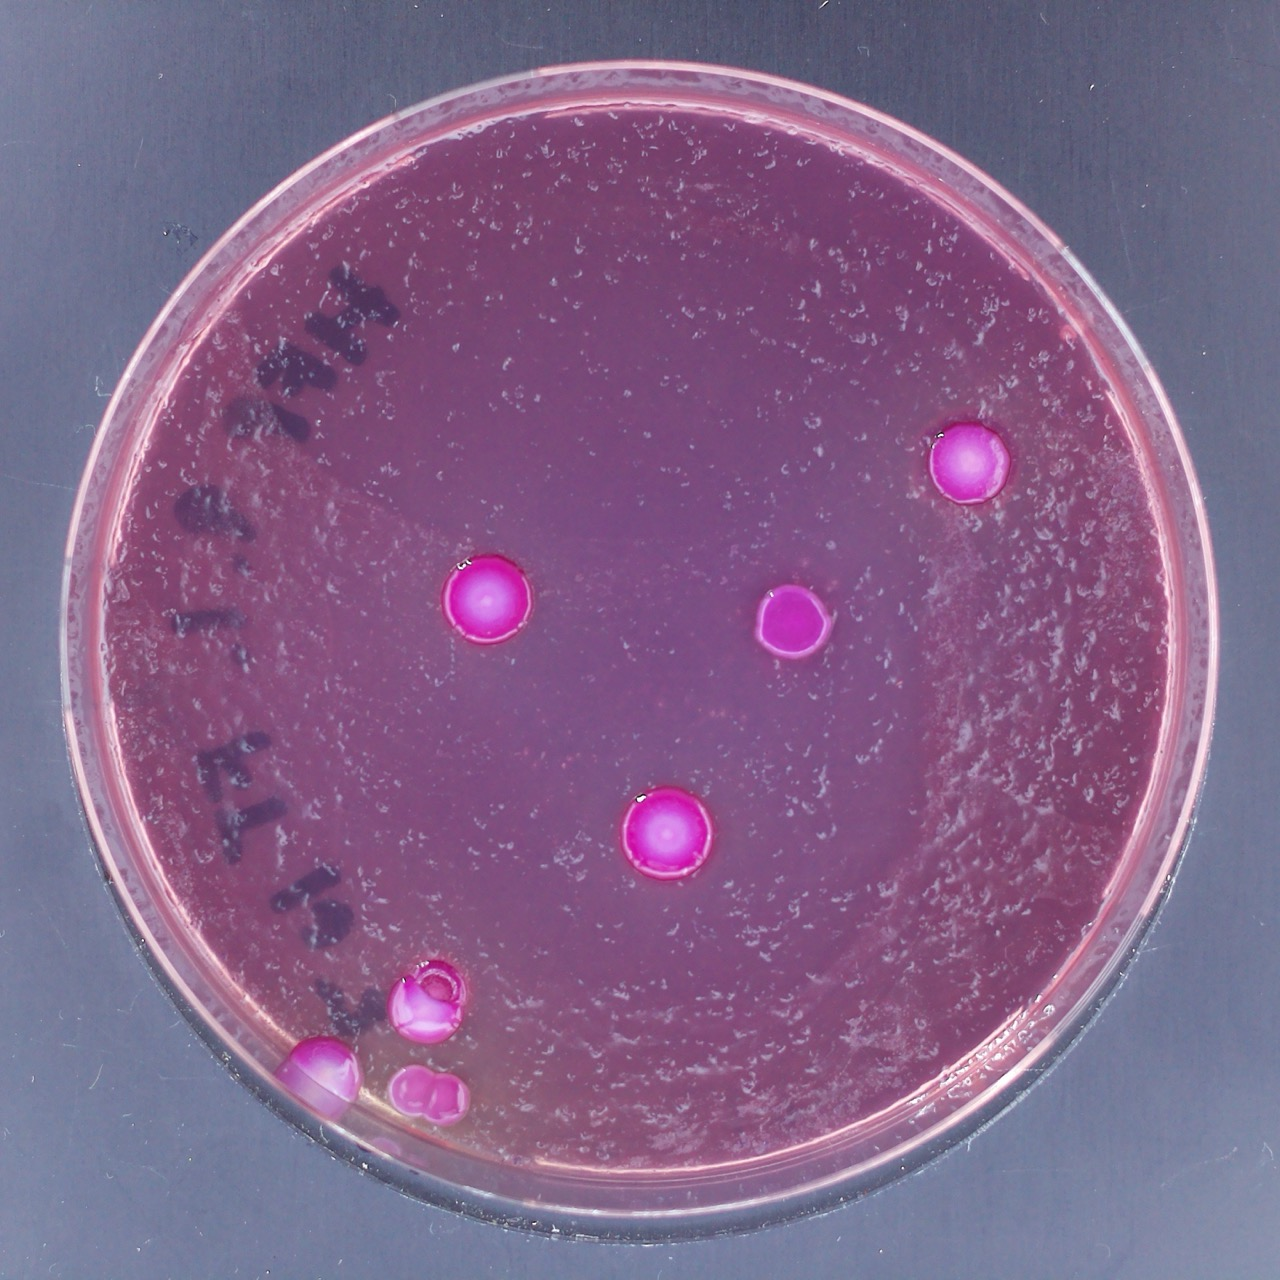
\includegraphics[width=0.2\textwidth]{assets/default_mmrsbpb_default_19012024140805} & 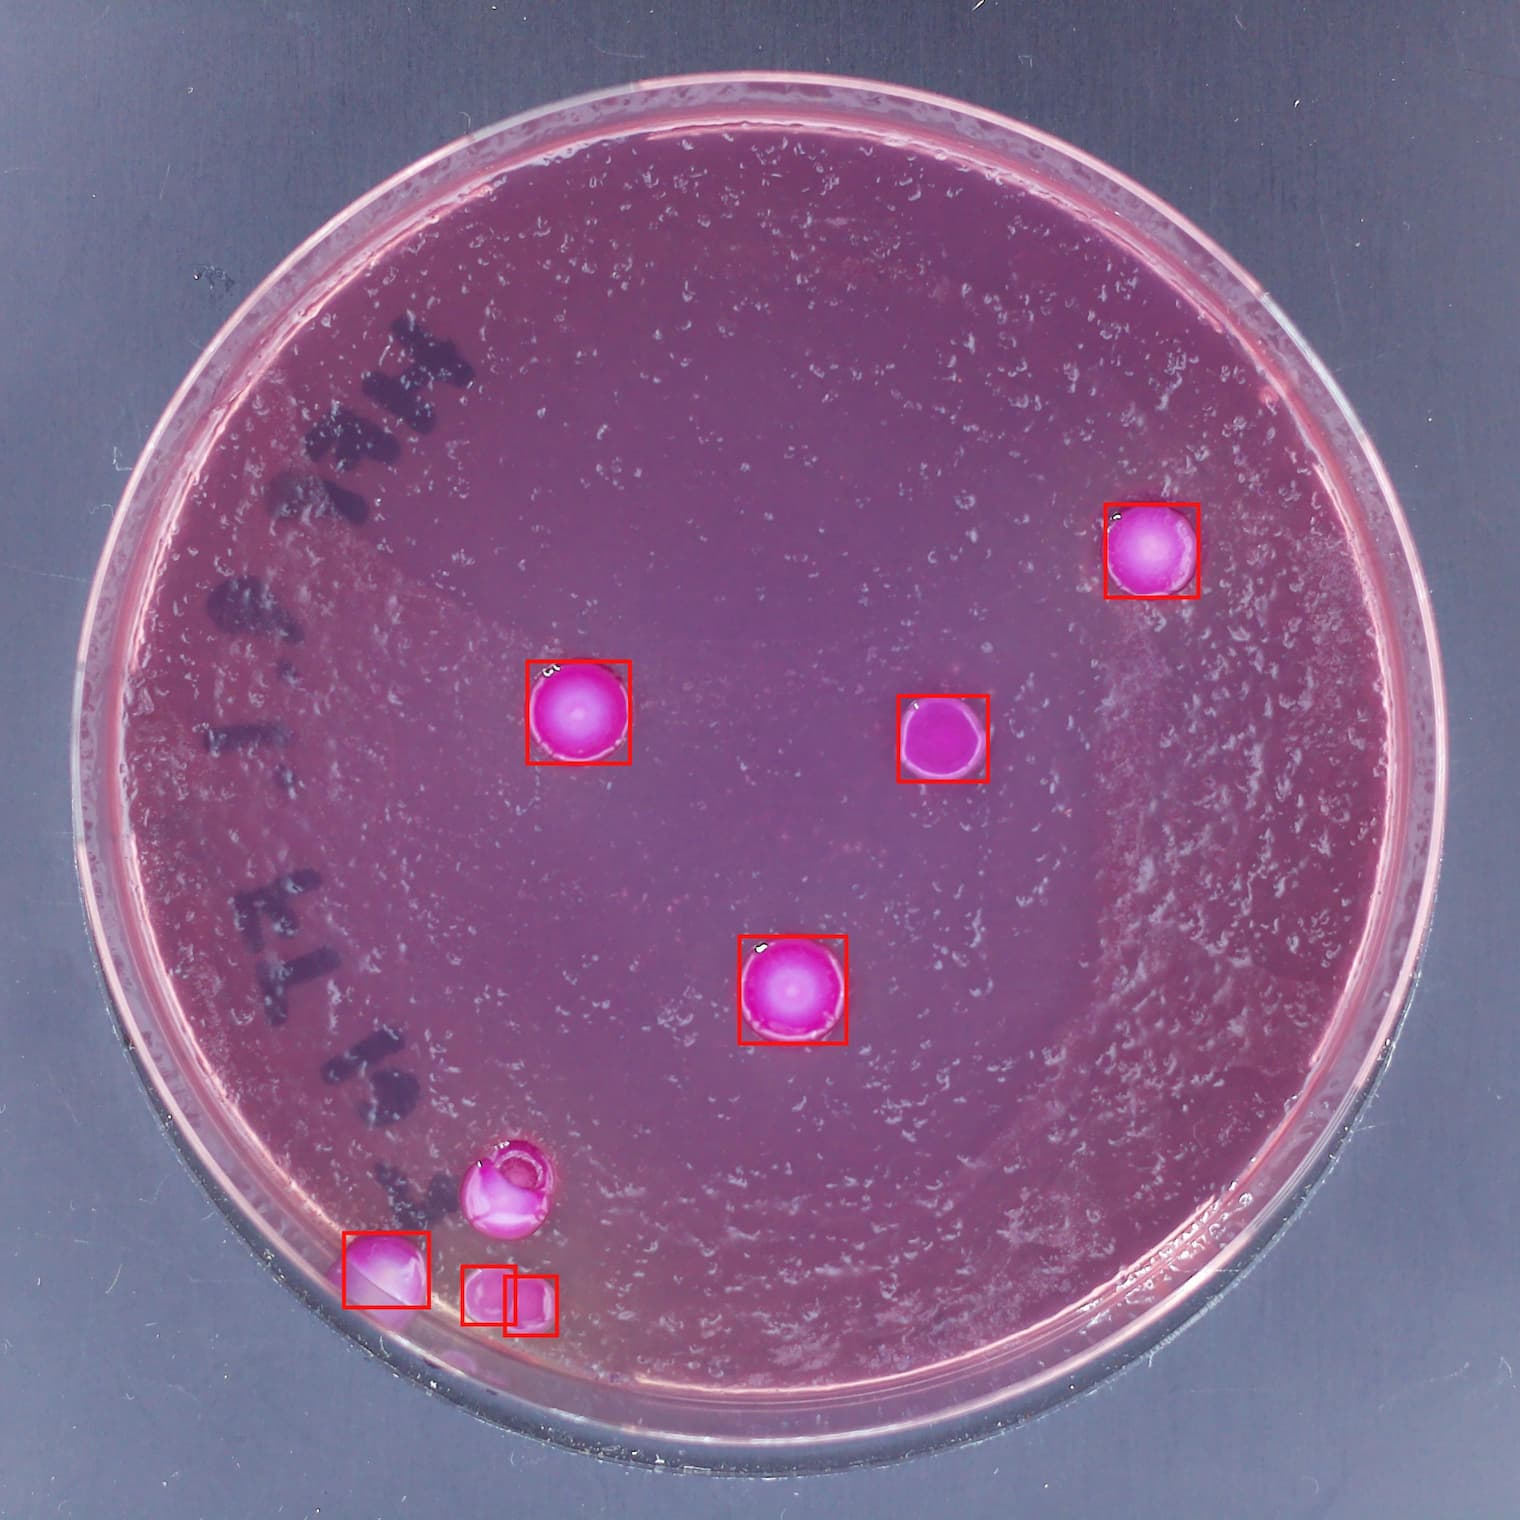
\includegraphics[width=0.2\textwidth]{assets/gt_default_mmrsbpb_default_19012024140805} & 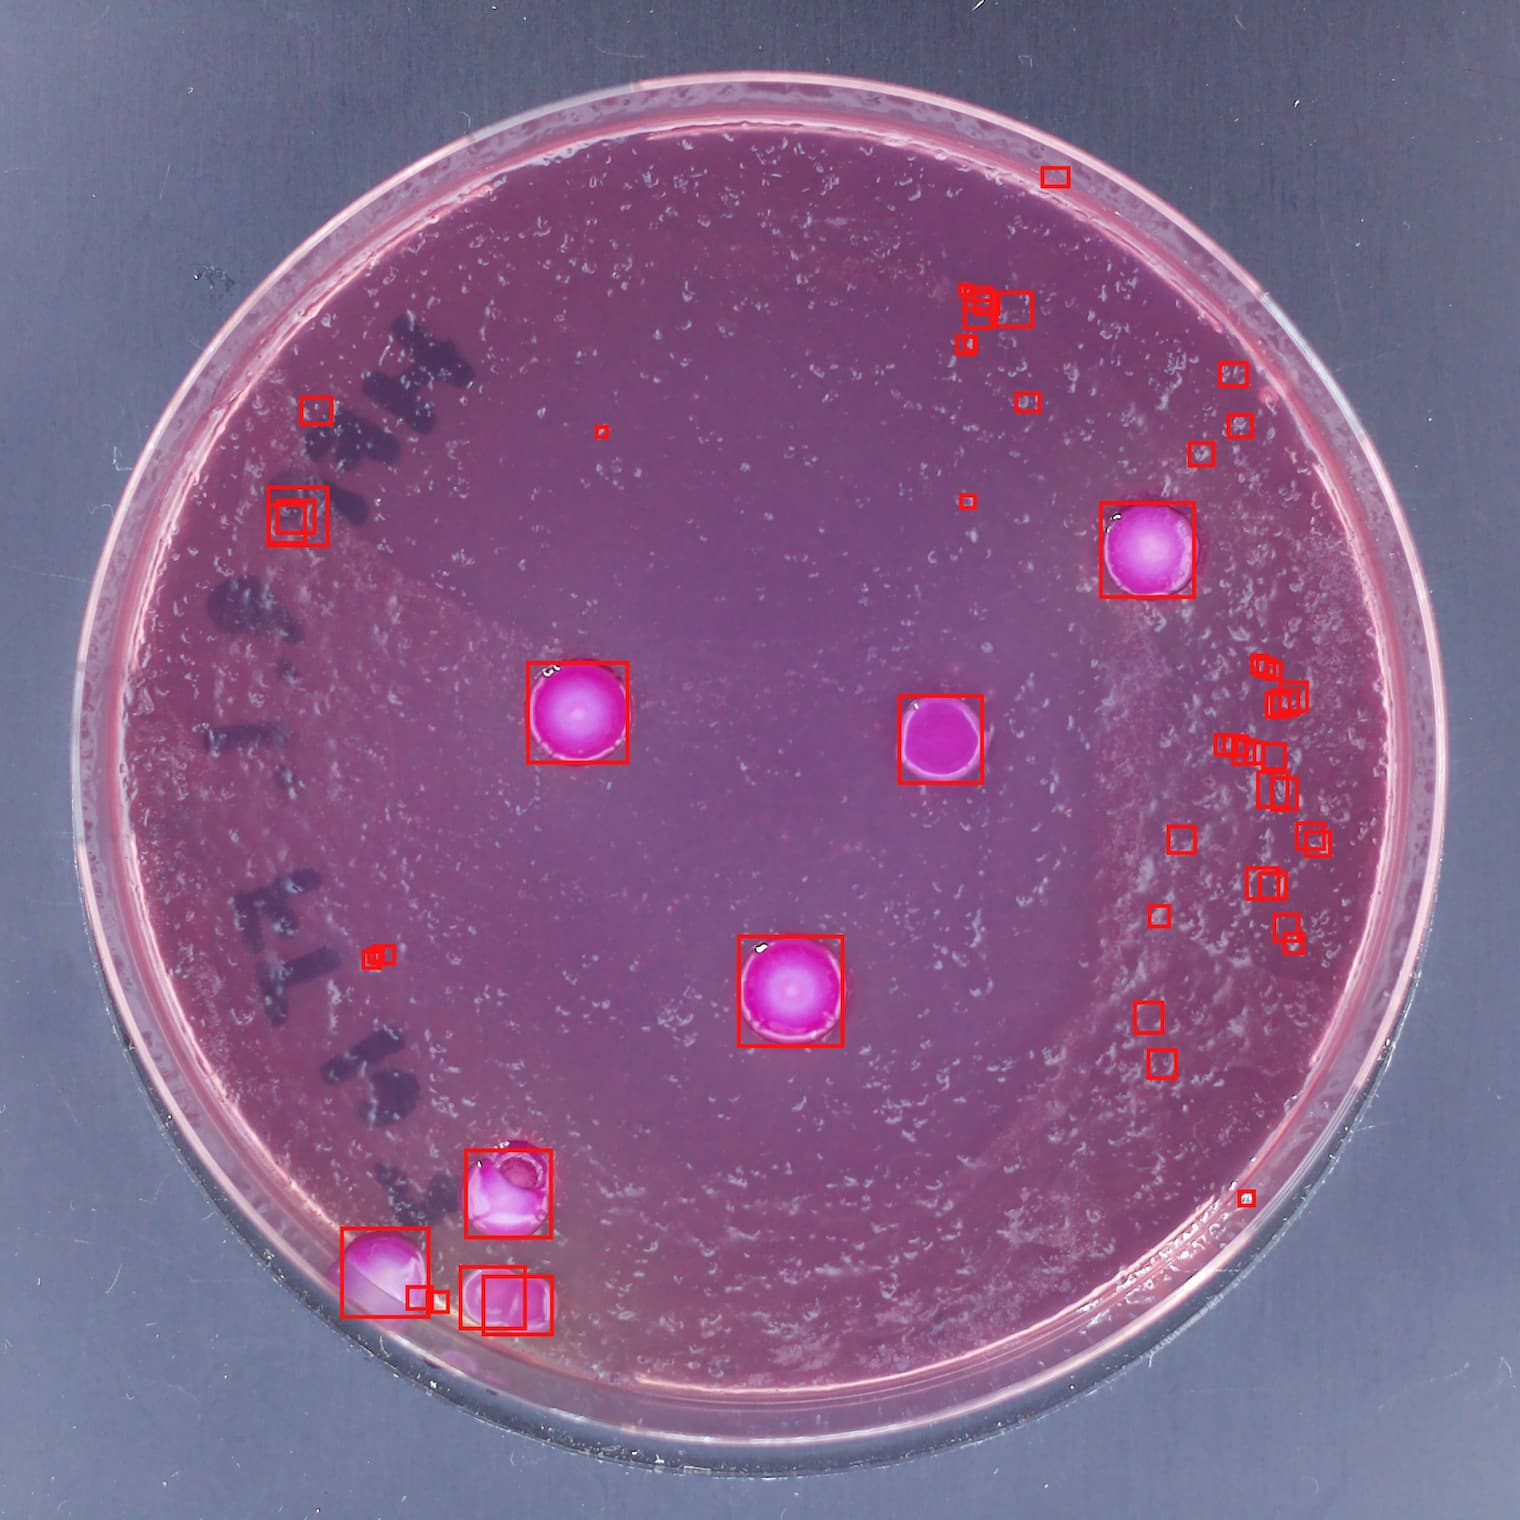
\includegraphics[width=0.2\textwidth]{assets/pred_default_mmrsbpb_default_19012024140805} & 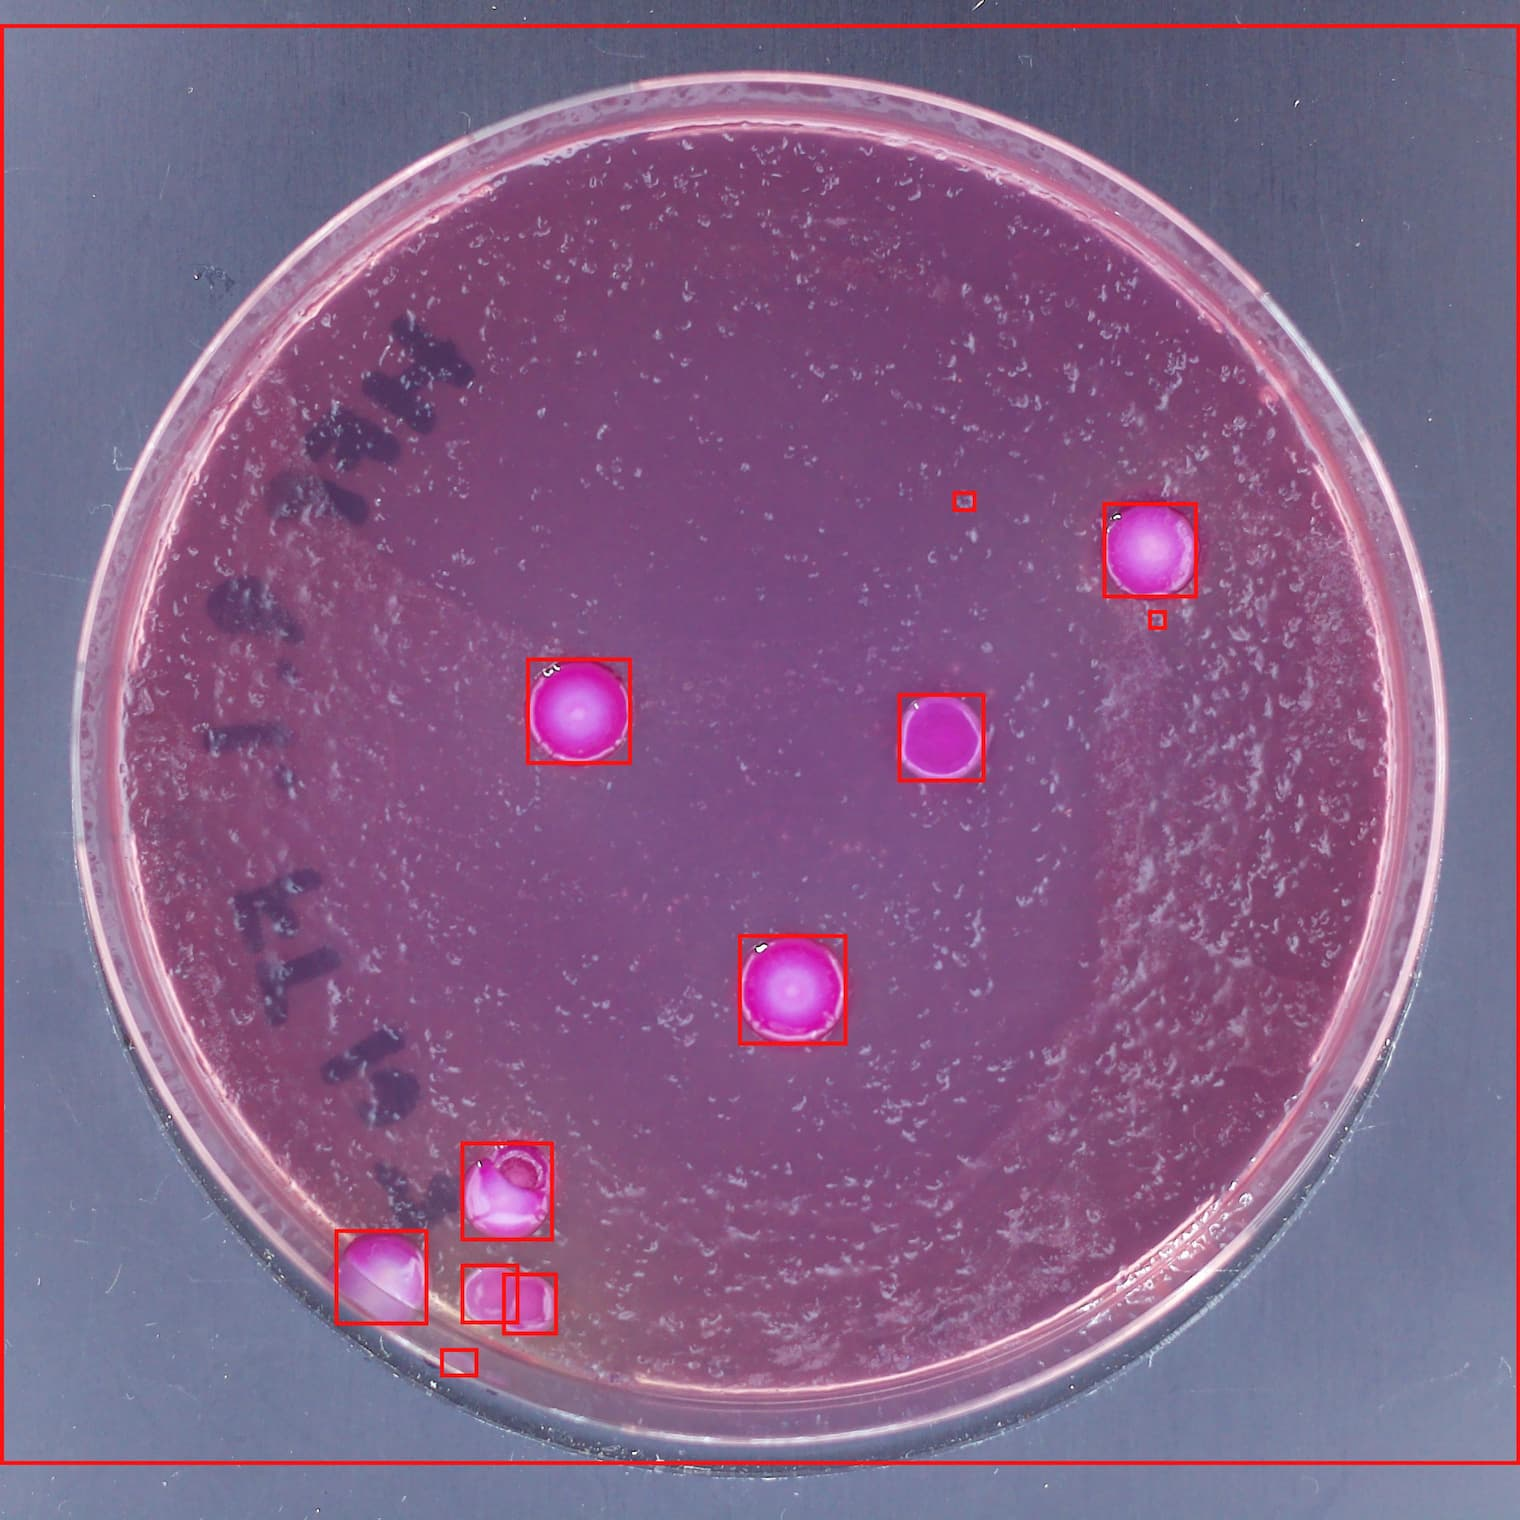
\includegraphics[width=0.2\textwidth]{assets/pt_pred_default_mmrsbpb_default_19012024140805} 
\\ \hline
\end{tabular}
\end{table}

Inspecting the performance visually (see Table \ref{tab:dataset_comparison_images}) shows that the inclusion of domain specific data (AGAR dataset) and non domain specific data (COCO dataset) in pre-training helps to reduce false positives. Also detection of smaller colonies and colonies that are close together improves. Small colonies in large numbers still propose a problem to the network, as seen in row 3 of the aforementioned table.

Other experiments included:

\begin{itemize}
	\item \textbf{Adjusting batch size and gradient clipping} did not yield any better results. The batch size that fills the available GPU memory (8) worked best and gradient clipping was not necessary there as training is already quite stable at that batch size. Gradient clipping only slows down convergence.
	\item \textbf{Trying out different image resolutions for Faster R-CNN} was also not beneficial. The standard configuration of resizing to 800x800px worked best, using higher resolutions did not improve the performance.
	\item \textbf{Using different optimizers} like Adam and AdamW did not yield better performance. Also their higher memory requirements meant the batch size had to be reduced, which introduced instability to the training.
\end{itemize}



